\documentclass[11pt,a4paper]{report}

% --- Encodage et langue ---
\usepackage[utf8]{inputenc}
\usepackage[T1]{fontenc}
\usepackage[french]{babel}

% --- Mise en page ---
\usepackage[top=2.2cm,bottom=2.2cm,left=2.2cm,right=2.2cm]{geometry}
\usepackage{setspace}
\onehalfspacing

% --- Graphiques, tableaux et couleurs ---
\usepackage{graphicx}
\usepackage{float}
\usepackage[table]{xcolor}
\usepackage{booktabs}
\usepackage{tabularx}
\usepackage{longtable}
\usepackage{amsmath}
\usepackage{amssymb}
\usepackage{tcolorbox}
\usepackage{titlesec}

% --- Palette officielle VoteUASZ ---
\definecolor{uaszgreen}{HTML}{047857}
\definecolor{uaszdark}{HTML}{065F46}
\definecolor{uaszlight}{HTML}{ECFDF5}
\definecolor{uaszblue}{HTML}{1D4ED8}
\definecolor{uaszslate}{HTML}{0F172A}
\definecolor{codebg}{HTML}{F8FAFC}
\definecolor{codeborder}{HTML}{CBD5E1}

% --- Styles des titres (design VoteUASZ) ---
\titleformat{\chapter}[display]
  {\normalfont\huge\bfseries\color{uaszdark}}
  {\colorbox{uaszgreen}{\parbox{0.96\textwidth}{\color{white}\large\ \chaptername\ \thechapter}}}
  {10pt}
  {\Huge\color{uaszslate}}
\titlespacing*{\chapter}{0pt}{-15pt}{18pt}

\titleformat{\section}
  {\normalfont\Large\bfseries\color{uaszdark}}
  {\textcolor{uaszblue}{\thesection}}{0.8em}{}
  [\vspace{-0.4em}\textcolor{uaszgreen}{\rule{\linewidth}{0.6pt}}]

\titleformat{\subsection}
  {\normalfont\large\bfseries\color{uaszslate}}
  {\textcolor{uaszgreen}{\thesubsection}}{0.6em}{}

% --- Boîtes VoteUASZ ---
\tcbuselibrary{skins,breakable}
\newtcolorbox{uaszbox}[1]{
  colback=uaszlight,
  colframe=uaszgreen,
  coltitle=white,
  fonttitle=\bfseries\small,
  title=#1,
  arc=3mm,
  boxrule=0.8pt,
  breakable
}

% --- En-têtes et pieds de page ---
\usepackage{fancyhdr}
\pagestyle{fancy}
\fancyhf{}
\fancyhead[L]{\small\textcolor{uaszdark}{\textbf{VoteUASZ}} \textcolor{gray}{| Mémoire de PFE}}
\fancyhead[R]{\small\textcolor{gray}{Ibrahima DIALLO (202300429)}}
\fancyfoot[L]{\small\textcolor{uaszgreen}{Université Assane Seck de Ziguinchor (UASZ)}}
\fancyfoot[R]{\small\textbf{\thepage}}
\renewcommand{\headrulewidth}{0.5pt}
\renewcommand{\footrulewidth}{0.5pt}

% --- Liens hypertextes ---
\usepackage[colorlinks=true,linkcolor=uaszdark,urlcolor=uaszblue,citecolor=uaszgreen]{hyperref}

\graphicspath{{images/}{../../report/figures/}{../../docs/uml/}}

\begin{document}

% ============================================================================
% PAGE DE GARDE — DESIGN VOTEUASZ
% ============================================================================
\begin{titlepage}
\begin{center}
    \begin{minipage}{0.2\textwidth}
        \centering
        
\includegraphics[height=2.1cm]{logo_uasz.png}
    \end{minipage}
    \hfill
    \begin{minipage}{0.55\textwidth}
        \centering
        {\small \textbf{RÉPUBLIQUE DU SÉNÉGAL}}\\
        {\footnotesize \textit{Un Peuple -- Un But -- Une Foi}}\\[0.2cm]
        {\small \textbf{\textcolor{uaszdark}{UNIVERSITÉ ASSANE SECK DE ZIGUINCHOR}}}\\
        {\footnotesize UFR Sciences et Technologies -- Département d'Informatique}
    \end{minipage}
    \hfill
    \begin{minipage}{0.2\textwidth}
        \centering
        
\includegraphics[height=2.1cm]{logo_vote_uasz.png}
    \end{minipage}

    \vspace{1.0cm}
    \begin{tcolorbox}[colback=uaszgreen,colframe=uaszdark,arc=4mm,boxrule=1pt]
        \centering
        {\Large \textbf{\color{white} MÉMOIRE DE PROJET DE FIN D'ÉTUDES}}
    \end{tcolorbox}

    \vspace{1.2cm}
    {\small \textsc{\textcolor{uaszblue}{\textbf{THÈME DU PROJET}}}}\\[0.4cm]
    {\LARGE \textbf{\textcolor{uaszslate}{Conception et Réalisation d'une Plateforme de Vote Électronique Sécurisée pour l'UASZ (\textcolor{uaszgreen}{VoteUASZ})}}}\\[1.5cm]

    \begin{tcolorbox}[colback=codebg,colframe=codeborder,arc=3mm,boxrule=0.8pt]
        \begin{minipage}{0.48\textwidth}
            \textbf{\textcolor{uaszdark}{Présenté par :}}\\
            \textbf{Ibrahima DIALLO}\\
            Matricule : \texttt{202300429}
        \end{minipage}
        \hfill
        \begin{minipage}{0.48\textwidth}
            \begin{flushright}
            \textbf{\textcolor{uaszdark}{Sous la direction de :}}\\
            \textbf{Monsieur TOURÉ}\\
            Encadreur académique
            \end{flushright}
        \end{minipage}
    \end{tcolorbox}

    \vfill
    {\normalsize \textbf{\textcolor{uaszdark}{Année universitaire : 2025 -- 2026}}}\\
    {\footnotesize Plateforme déployée : \url{https://vote-uasz-frontend.vercel.app}}
\end{center}
\end{titlepage}

% ============================================================================
% PAGES LIMINAIRES
% ============================================================================
\pagenumbering{roman}

\chapter*{Dédicace et Remerciements}
\addcontentsline{toc}{chapter}{Dédicace et Remerciements}
Je dédie ce travail à mes parents et à ma famille pour leur soutien constant.  
J'adresse mes sincères remerciements à mon encadreur, \textbf{Monsieur TOURÉ}, pour ses orientations rigoureuses et ses conseils méthodologiques, ainsi qu'aux enseignants du Département d'Informatique de l'UASZ et aux membres du jury.

\chapter*{Résumé et Abstract}
\addcontentsline{toc}{chapter}{Résumé et Abstract}
\begin{uaszbox}{Résumé technique}
\textbf{VoteUASZ} est une application web de vote électronique développée pour les scrutins de l'Université Assane Seck de Ziguinchor (\texttt{DELEGUE}, \texttt{DUFR}, \texttt{VICE\_RECTEUR}). Construite avec \textbf{Spring Boot 3.2.3 (Java 21)}, \textbf{Angular 17} et \textbf{PostgreSQL 16}, elle sépare structurellement l'émargement (\texttt{VoterAuditLog}) du bulletin (\texttt{Ballot}, sans clé étrangère vers \texttt{User}), chiffre le contenu du bulletin en \textbf{AES-256-GCM} (clé dérivée via PBKDF2WithHmacSHA256) et relie les bulletins par une chaîne d'empreintes \textbf{SHA-256} (\texttt{previousHash}). L'accès est protégé par \textbf{JWT HS256} avec \textbf{Refresh Token} rotatif, code \textbf{OTP} par e-mail (Brevo/SMTP), diffusion temps réel \textbf{STOMP} et génération de procès-verbal PDF (\textbf{OpenPDF}). La suite automatisée valide \textbf{154 tests backend} (couverture JaCoCo \textbf{65,17\,\%} en instructions et \textbf{70,87\,\%} en lignes, \textbf{0 violation Checkstyle}) et \textbf{28 tests frontend} (\textbf{0 échec}), pour un bundle initial de \textbf{430,96\,kB} (\textbf{111,06\,kB} transférés).

\medskip
\noindent\textbf{Mots-clés :} Vote électronique, Spring Boot, Angular, PostgreSQL, AES-256-GCM, SHA-256, JWT, OTP, WebSocket STOMP, UASZ.
\end{uaszbox}

\begin{uaszbox}{Abstract}
\textbf{VoteUASZ} is a secure e-voting web platform designed for Assane Seck University of Ziguinchor elections (\texttt{DELEGUE}, \texttt{DUFR}, \texttt{VICE\_RECTEUR}). Built with \textbf{Spring Boot 3.2.3 (Java 21)}, \textbf{Angular 17}, and \textbf{PostgreSQL 16}, it enforces ballot anonymity by isolating voter attendance (\texttt{VoterAuditLog}) from \textbf{AES-256-GCM} encrypted, \textbf{SHA-256} hash-chained ballots (\texttt{Ballot} without any foreign key to \texttt{User}). Security relies on \textbf{JWT HS256} with rotating \textbf{Refresh Tokens}, email \textbf{OTP}, \textbf{STOMP} live results, and \textbf{OpenPDF} reports. Automated verification passes \textbf{154 backend tests} (65.17\% JaCoCo instruction coverage, 70.87\% line coverage, 0 Checkstyle violations) and \textbf{28 Angular tests} (0 failures), with a \textbf{430.96\,kB} initial production bundle (111.06\,kB transfer size).

\medskip
\noindent\textbf{Keywords:} E-voting, Spring Boot, Angular, PostgreSQL, AES-256-GCM, SHA-256, JWT, OTP, WebSocket STOMP, UASZ.
\end{uaszbox}

\chapter*{Glossaire et Sigles}
\addcontentsline{toc}{chapter}{Glossaire et Sigles}
\begin{table}[H]
\centering
\small
\begin{tabularx}{\textwidth}{@{}lX@{}}
\toprule
\rowcolor{uaszlight}
\textbf{Sigle / Terme} & \textbf{Définition dans le cadre du projet} \\
\midrule
\textbf{AES-256-GCM} & \textit{Advanced Encryption Standard} 256 bits en mode Galois/Counter (confidentialité + tag d'authenticité 128 bits). \\
\textbf{API REST} & Interface de programmation applicative exposée sur HTTP(S) au format JSON (\texttt{/api/v1/**}). \\
\textbf{CORS} & \textit{Cross-Origin Resource Sharing}, politique de contrôle des origines autorisées par le navigateur. \\
\textbf{CSV} & \textit{Comma-Separated Values}, format utilisé pour l'import des électeurs et l'export du journal d'audit. \\
\textbf{DUFR} & Directeur d'Unité de Formation et de Recherche. \\
\textbf{JPA} & \textit{Jakarta Persistence API}, couche de mapping objet-relationnel (Hibernate). \\
\textbf{JWT} & \textit{JSON Web Token}, jeton d'authentification signé en \texttt{HS256}. \\
\textbf{OTP} & \textit{One-Time Password}, code à usage unique à 6 chiffres envoyé par e-mail (validité 5 min). \\
\textbf{PBKDF2} & \textit{Password-Based Key Derivation Function 2} (65\,536 itérations HMAC-SHA256). \\
\textbf{PV} & Procès-Verbal officiel de dépouillement généré au format PDF via OpenPDF. \\
\textbf{PWA} & \textit{Progressive Web App}, supportée côté Angular via \texttt{ngsw-config.json}. \\
\textbf{RBAC} & \textit{Role-Based Access Control} (\texttt{SUPER\_ADMIN}, \texttt{COMMISSION\_ELECTORALE}, \texttt{CANDIDAT}, \texttt{ELECTEUR}). \\
\textbf{SHA-256} & Fonction de hachage cryptographique utilisée pour le chaînage des bulletins, les jetons et l'audit IP. \\
\textbf{STOMP} & \textit{Simple Text Oriented Messaging Protocol} sur WebSocket (\texttt{/ws}) pour les résultats temps réel. \\
\textbf{UASZ} & Université Assane Seck de Ziguinchor. \\
\textbf{UFR} & Unité de Formation et de Recherche (\texttt{UFR\_SAT}, \texttt{UFR\_SJAG}, \texttt{UFR\_LL}). \\
\bottomrule
\end{tabularx}
\end{table}

\tableofcontents
\listoffigures
\listoftables

% ============================================================================
% CORPS DU MÉMOIRE
% ============================================================================
\clearpage
\pagenumbering{arabic}

\chapter*{Introduction Générale}
\addcontentsline{toc}{chapter}{Introduction Générale}

L'organisation traditionnelle sur papier des scrutins universitaires à l'Université Assane Seck de Ziguinchor (UASZ) mobilise d'importantes ressources logistiques, allonge les délais de dépouillement et limite la participation des électeurs éloignés du campus.

Le projet \textbf{VoteUASZ}, conçu et développé individuellement par l'étudiant dans le cadre de son Projet de Fin d'Études, propose une plateforme web sécurisée couvrant les scrutins de délégués de classe (\texttt{DELEGUE}), de directeurs d'UFR (\texttt{DUFR}) et de vice-recteur (\texttt{VICE\_RECTEUR}). L'architecture cherche un équilibre pragmatique entre \textbf{intégrité du scrutin} (unicité du vote, chaînage SHA-256 des bulletins) et \textbf{secret du suffrage} (isolation schématique entre l'identité de l'électeur et le bulletin enregistré).

Ce mémoire s'articule en trois chapitres :
\begin{itemize}
    \item Le \hyperref[chap:1]{\textbf{Chapitre 1}} présente la gestion du projet, l'analyse des besoins, le contrôle d'accès RBAC et le cycle de vie réel des scrutins.
    \item Le \hyperref[chap:2]{\textbf{Chapitre 2}} détaille la conception logicielle, les diagrammes UML et relationnels générés depuis le code, ainsi que l'analyse honnête des menaces et contre-mesures.
    \item Le \hyperref[chap:3]{\textbf{Chapitre 3}} décrit l'implémentation sécurisée, les interfaces réalisées, les métriques réelles de tests et de qualité, le déploiement cloud et le bilan critique par rapport au cahier des charges.
\end{itemize}

\chapter{Gestion de Projet, Spécification et Analyse des Besoins}

\section{Gestion et organisation du projet}

\subsection{Organisation des rôles et pratiques de développement}
Le projet \textbf{VoteUASZ} a été réalisé par un étudiant unique sous encadrement académique. Le tableau~\ref{tab:roles-projet} résume la répartition réelle des responsabilités observée sur le dépôt.

\begin{table}[H]
\centering
\caption{Répartition des rôles dans le projet}
\label{tab:roles-projet}
\small
\begin{tabularx}{\textwidth}{@{}llX@{}}
\toprule
\rowcolor{uaszlight}
\textbf{Intervenant} & \textbf{Rôle} & \textbf{Périmètre réel} \\
\midrule
Ibrahima DIALLO & Développeur unique (Full-Stack \& DevSecOps) & Conception UML, backend Spring Boot, frontend Angular, tests, Docker, CI/CD et déploiement Render/Vercel. \\
Monsieur TOURÉ & Encadreur académique & Orientation méthodologique et validation académique (\textit{[À COMPLÉTER PAR L'ÉTUDIANT : fréquence des séances de suivi]}). \\
\bottomrule
\end{tabularx}
\end{table}

\subsection{Workflow Git, intégration continue et qualité}
L'historique Git et la configuration du dépôt mettent en évidence les pratiques suivantes :
\begin{itemize}
    \item \textbf{Gestion de branches} : utilisation des branches principales \texttt{main} et \texttt{develop}, complétées par des branches thématiques (\texttt{feature/corrections-audit}, \texttt{feature/ameliorations-rapport}, \texttt{fix/tests-angular}, \texttt{fix/reset-password-ui}) fusionnées par \textit{Pull Requests}.
    \item \textbf{Intégration continue (CI)} : le workflow \texttt{.github/workflows/ci.yml} exécute automatiquement à chaque \textit{push}/\textit{PR} \texttt{mvn -B verify} (JDK 21) côté backend et \texttt{npx ng build --configuration production} (Node 20) côté frontend.
    \item \textbf{Qualité statique et couverture} : règles Checkstyle (\texttt{backend/checkstyle.xml}) et instrumentation JaCoCo (\texttt{0.8.11}) exécutées dans le cycle Maven.
    \item \textbf{Pratiques complémentaires} : \textit{[À COMPLÉTER PAR L'ÉTUDIANT : outil de suivi des tâches éventuel (Trello/Jira/GitHub Projects) et rythme des revues avec l'encadreur]}.
\end{itemize}

\subsection{Justification des choix technologiques}
\begin{table}[H]
\centering
\caption{Justification de la stack technique retenue}
\label{tab:choix-tech}
\small
\begin{tabularx}{\textwidth}{@{}llX@{}}
\toprule
\rowcolor{uaszlight}
\textbf{Couche} & \textbf{Technologie} & \textbf{Justification} \\
\midrule
Backend & Spring Boot 3.2.3 (Java 21) & Écosystème robuste (Spring Security, JPA, STOMP), typage fort et maintenance facilitée par les \texttt{switch} Java 21. \\
Frontend & Angular 17 + TailwindCSS & Architecture en composants \textit{standalone} avec \textit{lazy loading}, \textit{Guards} de routes et prise en charge PWA native. \\
Base de données & PostgreSQL 16 & SGBD relationnel ACID adapté aux contraintes d'unicité (\texttt{UNIQUE(user\_id, election\_id)}) et aux UUID natifs. \\
PDF \& Temps réel & OpenPDF 1.3.30 \& STOMP & Génération programmatique légère sans serveur Jasper externe ; diffusion temps réel sur WebSocket \texttt{/ws}. \\
Hébergement & Render + Vercel & Déploiement continu Docker (backend + PostgreSQL) et CDN statique avec réécriture \texttt{/api/**} (frontend). \\
\bottomrule
\end{tabularx}
\end{table}

\subsection{Planning réel issu de l'historique Git}
\begin{table}[H]
\centering
\caption{Chronologie réelle des jalons de développement (\texttt{git log})}
\label{tab:planning-git}
\small
\begin{tabularx}{\textwidth}{@{}llX@{}}
\toprule
\rowcolor{uaszlight}
\textbf{Période} & \textbf{Jalon} & \textbf{Livrables observés dans les commits} \\
\midrule
10 sept. 2026 & Socle initial & Code source initial VoteUASZ, sécurité OTP, WebSocket STOMP, export CSV audit. \\
26--30 sept. 2026 & Durcissement v1 & Corrections sécurité (JWT, CORS, brute-force), gestion des réclamations, optimisations UX. \\
22 oct. 2026 & Campagne \& statut & Espace candidat (publications de campagne), vérification du statut de vote. \\
13 nov. 2026 & Lots A--F \& Cloud & Fenêtre de vote, \texttt{RateLimitingFilter}, anonymat UUID/PBKDF2, \texttt{render.yaml}/\texttt{vercel.json}, API Brevo HTTPS. \\
17--18 nov. 2026 & Finalisation & Refresh tokens, chaînage SHA-256 des bulletins, réinitialisation mot de passe, refonte UI compacte et tests. \\
\bottomrule
\end{tabularx}
\end{table}

\section{Contexte, problématique et recueil des besoins}

À l'Université Assane Seck de Ziguinchor (UASZ), l'organisation manuelle des élections (délégués de classe, directeurs d'UFR, vice-recteur) engendre des coûts logistiques élevés, un dépouillement manuel lent et l'exclusion de fait des électeurs absents du campus.

\begin{uaszbox}{Recueil des besoins terrain}
\textit{[À COMPLÉTER PAR L'ÉTUDIANT : décrire ici les entretiens menés (services administratifs, étudiants, membres de commission) et l'observation éventuelle d'un scrutin papier à l'UASZ (dates, personnes interrogées, constats chiffrés).]}
\end{uaszbox}

\section{Acteurs, contrôle d'accès (RBAC) et types de scrutins}

L'application définit quatre rôles (\texttt{Role.java}) et trois types de scrutins (\texttt{TypeElection.java}), avec filtrage d'éligibilité dynamique dans \texttt{EligibilityService.java}.

\begin{table}[H]
\centering
\caption{Rôles RBAC et périmètre d'actions (\texttt{Role.java})}
\label{tab:rbac}
\small
\begin{tabularx}{\textwidth}{@{}lX@{}}
\toprule
\rowcolor{uaszlight}
\textbf{Rôle} & \textbf{Responsabilités principales} \\
\midrule
\texttt{SUPER\_ADMIN} & CRUD élections (en \texttt{CONFIGURATION}), transitions d'état, import CSV des comptes, consultation/export audit, export PV PDF. \\
\texttt{COMMISSION\_ELECTORALE} & Validation ou rejet motivé des candidatures, traitement des réclamations, consultation/export audit, export PV PDF. \\
\texttt{CANDIDAT} & Dépôt de candidature, publication unique de campagne (si approuvé), consultation des résultats, réclamations et vote (si éligible). \\
\texttt{ELECTEUR} & Consultation des scrutins et campagnes, vote sécurisé par OTP e-mail, consultation des résultats dès \texttt{DEPOUILLEMENT}, dépôt de réclamations. \\
\bottomrule
\end{tabularx}
\end{table}

\begin{table}[H]
\centering
\caption{Types de scrutins et règles d'éligibilité (\texttt{EligibilityService.java})}
\label{tab:types-scrutins}
\small
\begin{tabularx}{\textwidth}{@{}llX@{}}
\toprule
\rowcolor{uaszlight}
\textbf{Type} & \textbf{Corps électoral} & \textbf{Critères de ciblage} \\
\midrule
\texttt{DELEGUE} & \texttt{ETUDIANT} actifs & Correspondance exacte sur \texttt{UFR}, \texttt{Filière} et \texttt{Niveau}. \\
\texttt{DUFR} & Tous profils actifs & Correspondance sur l'\texttt{UFR} cible. \\
\texttt{VICE\_RECTEUR} & Tous utilisateurs actifs & Scrutin global sans ciblage restrictif. \\
\bottomrule
\end{tabularx}
\end{table}

\section{Besoins fonctionnels et non fonctionnels}

\begin{table}[H]
\centering
\caption{Synthèse des besoins fonctionnels et non fonctionnels}
\label{tab:besoins}
\small
\begin{tabularx}{\textwidth}{@{}llX@{}}
\toprule
\rowcolor{uaszlight}
\textbf{Catégorie} & \textbf{Code} & \textbf{Exigence spécifiée} \\
\midrule
Fonctionnel & BF-01 & Import en masse des électeurs/candidats par CSV sans mot de passe en clair dans le fichier. \\
Fonctionnel & BF-02 & Gestion des scrutins selon une machine à états stricte et dépôt/validation des candidatures. \\
Fonctionnel & BF-03 & Vote unique à distance validé par OTP e-mail et jeton temporaire (\texttt{VoteToken}). \\
Fonctionnel & BF-04 & Dépouillement temps réel (STOMP), export PV PDF (OpenPDF) et gestion des réclamations (48\,h). \\
Non fonctionnel & BNF-01 & Anonymat structurel du bulletin (\texttt{Ballot} sans clé étrangère vers \texttt{User}). \\
Non fonctionnel & BNF-02 & Protection contre la force brute (\texttt{RateLimitingFilter}, verrouillage après 5 échecs). \\
Non fonctionnel & BNF-03 & Interface responsive (desktop et mobile) avec support PWA. \\
\bottomrule
\end{tabularx}
\end{table}

\section{Cycle de vie réel d'une élection}

La classe \texttt{ElectionStateMachine.java} impose une progression séquentielle stricte à \textbf{6 états} (\texttt{ElectionStatus}). Tout saut d'étape ou retour arrière lève une exception traduite en HTTP \texttt{409 Conflict}. La figure~\ref{fig:state-machine} illustre ce diagramme d'états extrait du code.

\begin{figure}[H]
    \centering
    \includegraphics[width=0.92\textwidth,height=0.48\textheight,keepaspectratio]{state-machine-election.pdf}
    \caption{Machine à états réelle d'une élection (\texttt{ElectionStateMachine.java})}
    \label{fig:state-machine}
\end{figure}

\chapter{Conception}

\section{Architecture logicielle et déploiement}

L'architecture de \textbf{VoteUASZ} suit un modèle 3-tiers découplé :
\begin{itemize}
    \item \textbf{Frontend (Angular 17 / Vercel)} : 11 composants \textit{standalone} avec chargement paresseux, \textit{Guards} RBAC, intercepteur JWT (\texttt{jwtInterceptor}), client STOMP/RxJS, graphiques \textbf{Chart.js} et Service Worker PWA (\texttt{ngsw-config.json}).
    \item \textbf{Backend (Spring Boot 3.2.3 / Java 21 / Render)} : filtres \texttt{RateLimitingFilter} et \texttt{JwtAuthenticationFilter}, 9 contrôleurs REST (\texttt{/api/v1/**}), 12 services métier et broker WebSocket STOMP (\texttt{/ws}).
    \item \textbf{Persistance \& Messagerie} : \textbf{PostgreSQL 16} en production (H2 en tests) et envoi d'e-mails via l'API HTTPS Brevo (ou SMTP MailHog en environnement local Docker).
\end{itemize}

La figure~\ref{fig:components-packages} présente l'organisation des composants et packages du dépôt, et la figure~\ref{fig:deployment} détaille l'architecture de déploiement issue de \texttt{render.yaml}, \texttt{vercel.json} et \texttt{docker-compose.yml}.

\begin{figure}[H]
    \centering
    \includegraphics[width=0.95\textwidth,height=0.50\textheight,keepaspectratio]{components-packages.pdf}
    \caption{Diagramme de composants et packages (\texttt{frontend/src/app} et \texttt{sn.uasz.vote})}
    \label{fig:components-packages}
\end{figure}

\begin{figure}[H]
    \centering
    \includegraphics[width=0.95\textwidth,height=0.45\textheight,keepaspectratio]{deployment.pdf}
    \caption{Diagramme de déploiement (Vercel, Render, PostgreSQL 16, Brevo et Docker local)}
    \label{fig:deployment}
\end{figure}

\section{Modélisation UML et base de données}

\subsection{Cas d'utilisation et workflow global}
La figure~\ref{fig:use-case} synthétise les cas d'utilisation par rôle à partir des contrôleurs REST. La figure~\ref{fig:activity-workflow} modélise le déroulement complet d'un scrutin de sa création à l'export du procès-verbal.

\begin{figure}[H]
    \centering
    \includegraphics[width=0.95\textwidth,height=0.50\textheight,keepaspectratio]{use-case-global.pdf}
    \caption{Diagramme de cas d'utilisation global de VoteUASZ}
    \label{fig:use-case}
\end{figure}

\begin{figure}[H]
    \centering
    \includegraphics[width=0.82\textwidth,height=0.55\textheight,keepaspectratio]{activity-election-workflow.pdf}
    \caption{Diagramme d'activités du workflow complet d'une élection}
    \label{fig:activity-workflow}
\end{figure}

\subsection{Diagrammes de séquence : authentification et vote complet}
Les figures~\ref{fig:seq-auth} et~\ref{fig:seq-vote} décrivent respectivement la cinématique d'authentification (JWT + Refresh Token rotatif + réinitialisation) et le protocole de vote en trois étapes (\texttt{/vote/request-otp}, \texttt{/vote/verify-otp}, \texttt{/vote/submit}).

\begin{figure}[H]
    \centering
    \includegraphics[width=0.95\textwidth,height=0.48\textheight,keepaspectratio]{sequence-auth-otp.pdf}
    \caption{Diagramme de séquence : authentification JWT, Refresh Token et réinitialisation}
    \label{fig:seq-auth}
\end{figure}

\begin{figure}[H]
    \centering
    \includegraphics[width=0.95\textwidth,height=0.55\textheight,keepaspectratio]{sequence-vote-complet.pdf}
    \caption{Diagramme de séquence : flux complet de vote sécurisé et diffusion STOMP}
    \label{fig:seq-vote}
\end{figure}

\subsection{Diagramme de classes et modèle logique de données (MLD)}
La base de données s'appuie sur \textbf{11 entités JPA} et \textbf{6 énumérations} (tableau~\ref{tab:entities}, figures~\ref{fig:class-diagram} et~\ref{fig:mld-schema}).

\begin{table}[H]
\centering
\caption{Les 11 entités JPA du dépôt (\texttt{sn.uasz.vote.entity})}
\label{tab:entities}
\small
\begin{tabularx}{\textwidth}{@{}llX@{}}
\toprule
\rowcolor{uaszlight}
\textbf{Entité} & \textbf{Table} & \textbf{Rôle et champs clés} \\
\midrule
\texttt{User} & \texttt{users} & \texttt{matricule}, \texttt{email} (uniques), \texttt{role}, \texttt{typeElecteur}, \texttt{ufr/filiere/niveau}, \texttt{failedLoginAttempts}, \texttt{lockedUntil}. \\
\texttt{Election} & \texttt{elections} & \texttt{titre}, \texttt{type}, \texttt{statut}, \texttt{dateDebut}, \texttt{dateFin}, cibles UFR/filière/niveau. \\
\texttt{Candidature} & \texttt{candidatures} & \texttt{nomListe}, URLs (\texttt{photoUrl}, \texttt{programmePdf}, \texttt{cvUrl}), \texttt{statut}, \texttt{motifRejet}. \\
\texttt{CampaignPost} & \texttt{campaign\_posts} & Publications de campagne (\texttt{titre}, \texttt{contenu}, \texttt{afficheUrl}, \texttt{videoEmbedUrl}). \\
\texttt{VoteOTP} & \texttt{vote\_otps} & \texttt{codeHash} (BCrypt), \texttt{expiresAt} (5\,min), \texttt{used}, \texttt{attemptsCount}. \\
\texttt{VoteToken} & \texttt{vote\_tokens} & \texttt{tokenHash} (SHA-256, unique), \texttt{expiresAt} (10\,min), \texttt{used}. \\
\texttt{Ballot} & \texttt{ballots} & \texttt{id} (\texttt{UUID}), \texttt{candidatureId}, \texttt{encryptedPayload}, \texttt{ballotHash}, \texttt{previousHash}, \texttt{sequenceNumber}. \\
\texttt{VoterAuditLog} & \texttt{voter\_audit\_logs} & \texttt{votedAt} (tronqué à l'heure), \texttt{ipHash}, contrainte \texttt{UNIQUE(user\_id, election\_id)}. \\
\texttt{Complaint} & \texttt{complaints} & \texttt{sujet}, \texttt{description}, \texttt{statut}, \texttt{reponseCommission}, \texttt{createdAt}. \\
\texttt{RefreshToken} & \texttt{refresh\_tokens} & \texttt{tokenHash} (SHA-256, unique), \texttt{expiresAt} (7\,j), \texttt{revoked}. \\
\texttt{PasswordResetToken} & \texttt{password\_reset\_tokens} & \texttt{codeHash} (BCrypt), \texttt{expiresAt} (15\,min), \texttt{used}. \\
\bottomrule
\end{tabularx}
\end{table}

\begin{figure}[H]
    \centering
    \includegraphics[width=0.95\textwidth,height=0.58\textheight,keepaspectratio]{class-diagram.pdf}
    \caption{Diagramme de classes des 11 entités JPA (dissociation \texttt{Ballot}/\texttt{User})}
    \label{fig:class-diagram}
\end{figure}

\begin{figure}[H]
    \centering
    \includegraphics[width=0.95\textwidth,height=0.55\textheight,keepaspectratio]{mld-schema.pdf}
    \caption{Modèle Logique de Données (MLD) PostgreSQL soulignant l'absence de clé entre \texttt{ballots} et \texttt{users}}
    \label{fig:mld-schema}
\end{figure}

\section{Analyse des menaces, contre-mesures et limites cryptographiques}

Le tableau~\ref{tab:menaces} synthétise les menaces identifiées et les mécanismes réellement implémentés dans le code, sans surestimer les garanties cryptographiques.

\begin{table}[H]
\centering
\caption{Analyse Menaces / Contre-mesures / Limites réelles du code}
\label{tab:menaces}
\small
\begin{tabularx}{\textwidth}{@{}lXX@{}}
\toprule
\rowcolor{uaszlight}
\textbf{Menace} & \textbf{Contre-mesure implémentée} & \textbf{Limite résiduelle honnête} \\
\midrule
Double vote & Contrainte \texttt{UNIQUE(user\_id, election\_id)} sur \texttt{voter\_audit\_logs}, vérification préalable et invalidation du \texttt{VoteToken}. & Protection applicative et SGBD complète pour un compte donné. \\
Force brute / DDoS applicatif & \texttt{RateLimitingFilter} (20\,req/min/IP sur login et OTP), verrouillage 5\,min après 5 échecs, \texttt{ClientIpResolver} anti-spoofing proxy. & Fenêtre en mémoire JVM (non partagée si plusieurs instances backend). \\
Rupture du secret du vote & Absence totale de clé étrangère entre \texttt{ballots} et \texttt{users} ; \texttt{Ballot.id} en \texttt{UUID} sans \texttt{createdAt} ; \texttt{votedAt} tronqué à l'heure et IP salée. & \textbf{Corrélation d'ordre possible} : dans \texttt{VotingService.submitVote()}, \texttt{VoterAuditLog} (ID séquentiel) et \texttt{Ballot.sequenceNumber} sont insérés dans la même transaction. \\
Accès au contenu des bulletins & Chiffrement \textbf{AES-256-GCM} (PBKDF2WithHmacSHA256, 65\,536 itérations, IV 12\,octets). & \textbf{Clé détenue par le serveur} (\texttt{CRYPTO\_SECRET}) : le serveur peut déchiffrer à tout moment ; de plus, \texttt{candidatureId} est stocké en clair dans \texttt{ballots} pour le décompte SQL temps réel. \\
Altération silencieuse des bulletins & Chaînage \textbf{SHA-256} (\texttt{previousHash} depuis \texttt{"GENESIS"}) vérifié par \texttt{AuditService.verifyBallotChain()}. & \textbf{Aucune signature asymétrique RSA} ni reçu individuel vérifiable par l'électeur ; le PV PDF OpenPDF n'est pas signé numériquement (X.509). \\
\bottomrule
\end{tabularx}
\end{table}

\section{Patrons de conception et stack technique}

\begin{table}[H]
\centering
\caption{Patrons de conception réels et versions exactes des dépendances}
\label{tab:patterns-stack}
\small
\begin{tabularx}{\textwidth}{@{}llX@{}}
\toprule
\rowcolor{uaszlight}
\textbf{Pattern / Couche} & \textbf{Statut / Version} & \textbf{Implémentation réelle dans le dépôt} \\
\midrule
\textbf{Observer} & Présent & Broker STOMP (\texttt{SimpMessagingTemplate}) + \texttt{BehaviorSubject} Angular. \\
\textbf{Repository / DTO / Builder} & Présents & 11 \texttt{JpaRepository}, DTOs dédiés, Lombok \texttt{@Builder}, IoC Spring. \\
\textit{State / Strategy} & \textit{Switch sur enum} & \texttt{ElectionStateMachine} et \texttt{EligibilityService} utilisent des \texttt{switch} Java 21. \\
\midrule
Backend & Java 21 / Boot 3.2.3 & JJWT \texttt{0.11.5}, OpenPDF \texttt{1.3.30}, springdoc \texttt{2.3.0}, JaCoCo \texttt{0.8.11}, Checkstyle \texttt{3.3.1}. \\
Frontend & Angular \texttt{\^{}17.3.0} & RxJS \texttt{\~{}7.8.0}, TailwindCSS \texttt{\^{}3.4.19}, Chart.js \texttt{\^{}4.5.1}, STOMP.js \texttt{\^{}7.3.0}. \\
\bottomrule
\end{tabularx}
\end{table}

\chapter{Implémentation, Tests et Résultats}

\section{Authentification JWT, Refresh Token et sécurité réseau}

\begin{itemize}
    \item \textbf{JWT (\texttt{HS256}) et Refresh Token rotatif} : jeton d'accès valable 24\,h (\texttt{JwtTokenProvider.java}), associé à un \texttt{RefreshToken} de 7\,jours stocké haché en \textbf{SHA-256} (\texttt{/auth/refresh}, \texttt{/auth/logout}).
    \item \textbf{Protection anti-force brute} : verrouillage de 5\,minutes après 5 échecs de connexion et filtre \texttt{RateLimitingFilter} (20\,req/min/IP sur \texttt{/auth/login}, \texttt{/vote/request-otp}, \texttt{/vote/verify-otp}), avec résolution d'IP réelle derrière proxy (\texttt{ClientIpResolver}).
    \item \textbf{Réinitialisation} : \texttt{/auth/forgot-password} génère un code à 6 chiffres (validité 15\,min, hash BCrypt) et renvoie une réponse neutre anti-énumération ; \texttt{/auth/reset-password} met à jour le mot de passe et révoque les sessions actives.
\end{itemize}

\section{Vote sécurisé, chiffrement AES-256-GCM et chaînage SHA-256}

Le protocole de vote (\texttt{VotingService.java}, L94--L228) s'exécute en trois étapes :
\begin{enumerate}
    \item \textbf{Demande d'OTP (\texttt{/vote/request-otp})} : vérification de la fenêtre temporelle, de l'éligibilité, de l'unicité, du quota (5/h) et du cooldown (60\,s) ; génération d'un code 6 chiffres via \texttt{SecureRandom}, haché en \textbf{BCrypt} et envoyé par e-mail (Brevo HTTPS API en production, SMTP MailHog en local).
    \item \textbf{Vérification OTP (\texttt{/vote/verify-otp})} : maximum 5 tentatives (validité 5\,min) ; délivre un \texttt{VoteToken} SHA-256 à usage unique (validité 10\,min).
    \item \textbf{Dépôt du bulletin (\texttt{/vote/submit})} : transaction \texttt{@Transactional} chiffrant le choix en \textbf{AES-256-GCM} (IV aléatoire 12\,octets, clé dérivée par \textbf{PBKDF2WithHmacSHA256} sur 65\,536 itérations), calculant l'empreinte chaînée \textbf{SHA-256}, enregistrant l'émargement (\texttt{VoterAuditLog}) et invalidant le \texttt{VoteToken}.
\end{enumerate}

\begin{uaszbox}{Chaînage SHA-256 des bulletins (\texttt{Ballot} \& \texttt{AuditService})}
Chaque bulletin référence l'empreinte du bulletin précédent (\texttt{previousHash}, initialisée à \texttt{"GENESIS"}) et un numéro de séquence :
$$\text{ballotHash}_n = \text{SHA-256}\left(\text{previousHash}_n \,\|\, \text{encryptedPayload}_n \,\|\, \text{sequenceNumber}_n\right)$$
\texttt{AuditService.verifyBallotChain()} vérifie l'intégrité séquentielle de la chaîne. Lors de la validation locale sur le scrutin \textit{L3 Informatique 2026} (25 votes), \texttt{verifyBallotChain()} a retourné \texttt{chainValid = true}.
\end{uaszbox}

\section{Temps réel, PV PDF et réclamations}

\begin{itemize}
    \item \textbf{WebSocket STOMP} : diffusion des résultats sur \texttt{/topic/results/\{id\}} sécurisée par \texttt{ChannelInterceptor}, alimentant automatiquement les graphiques \textbf{Chart.js} côté Angular.
    \item \textbf{Procès-Verbal PDF} : génération programmatique via \textbf{OpenPDF 1.3.30} (\texttt{PdfReportService.java}) dès l'état \texttt{CLOTURE}.
    \item \textbf{Réclamations} : dépôt autorisé uniquement aux états \texttt{PUBLICATION} et \texttt{CLOTURE} dans un délai de 48\,heures après \texttt{dateFin} (\texttt{ComplaintService.java}).
\end{itemize}

\section{Interfaces applicatives réalisées}

Les captures ci-après ont été réalisées sur l'environnement local peuplé avec des données fictives réalistes de l'UASZ (desktop \texttt{1440x900} et mobile \texttt{390x844}).

\subsection{Authentification et réinitialisation}
Les figures~\ref{fig:login-desktop}, \ref{fig:login-mobile}, \ref{fig:forgot} et~\ref{fig:reset} illustrent la page de connexion compacte (desktop et mobile) ainsi que les modes de réinitialisation de mot de passe.

\begin{figure}[H]
    \centering
    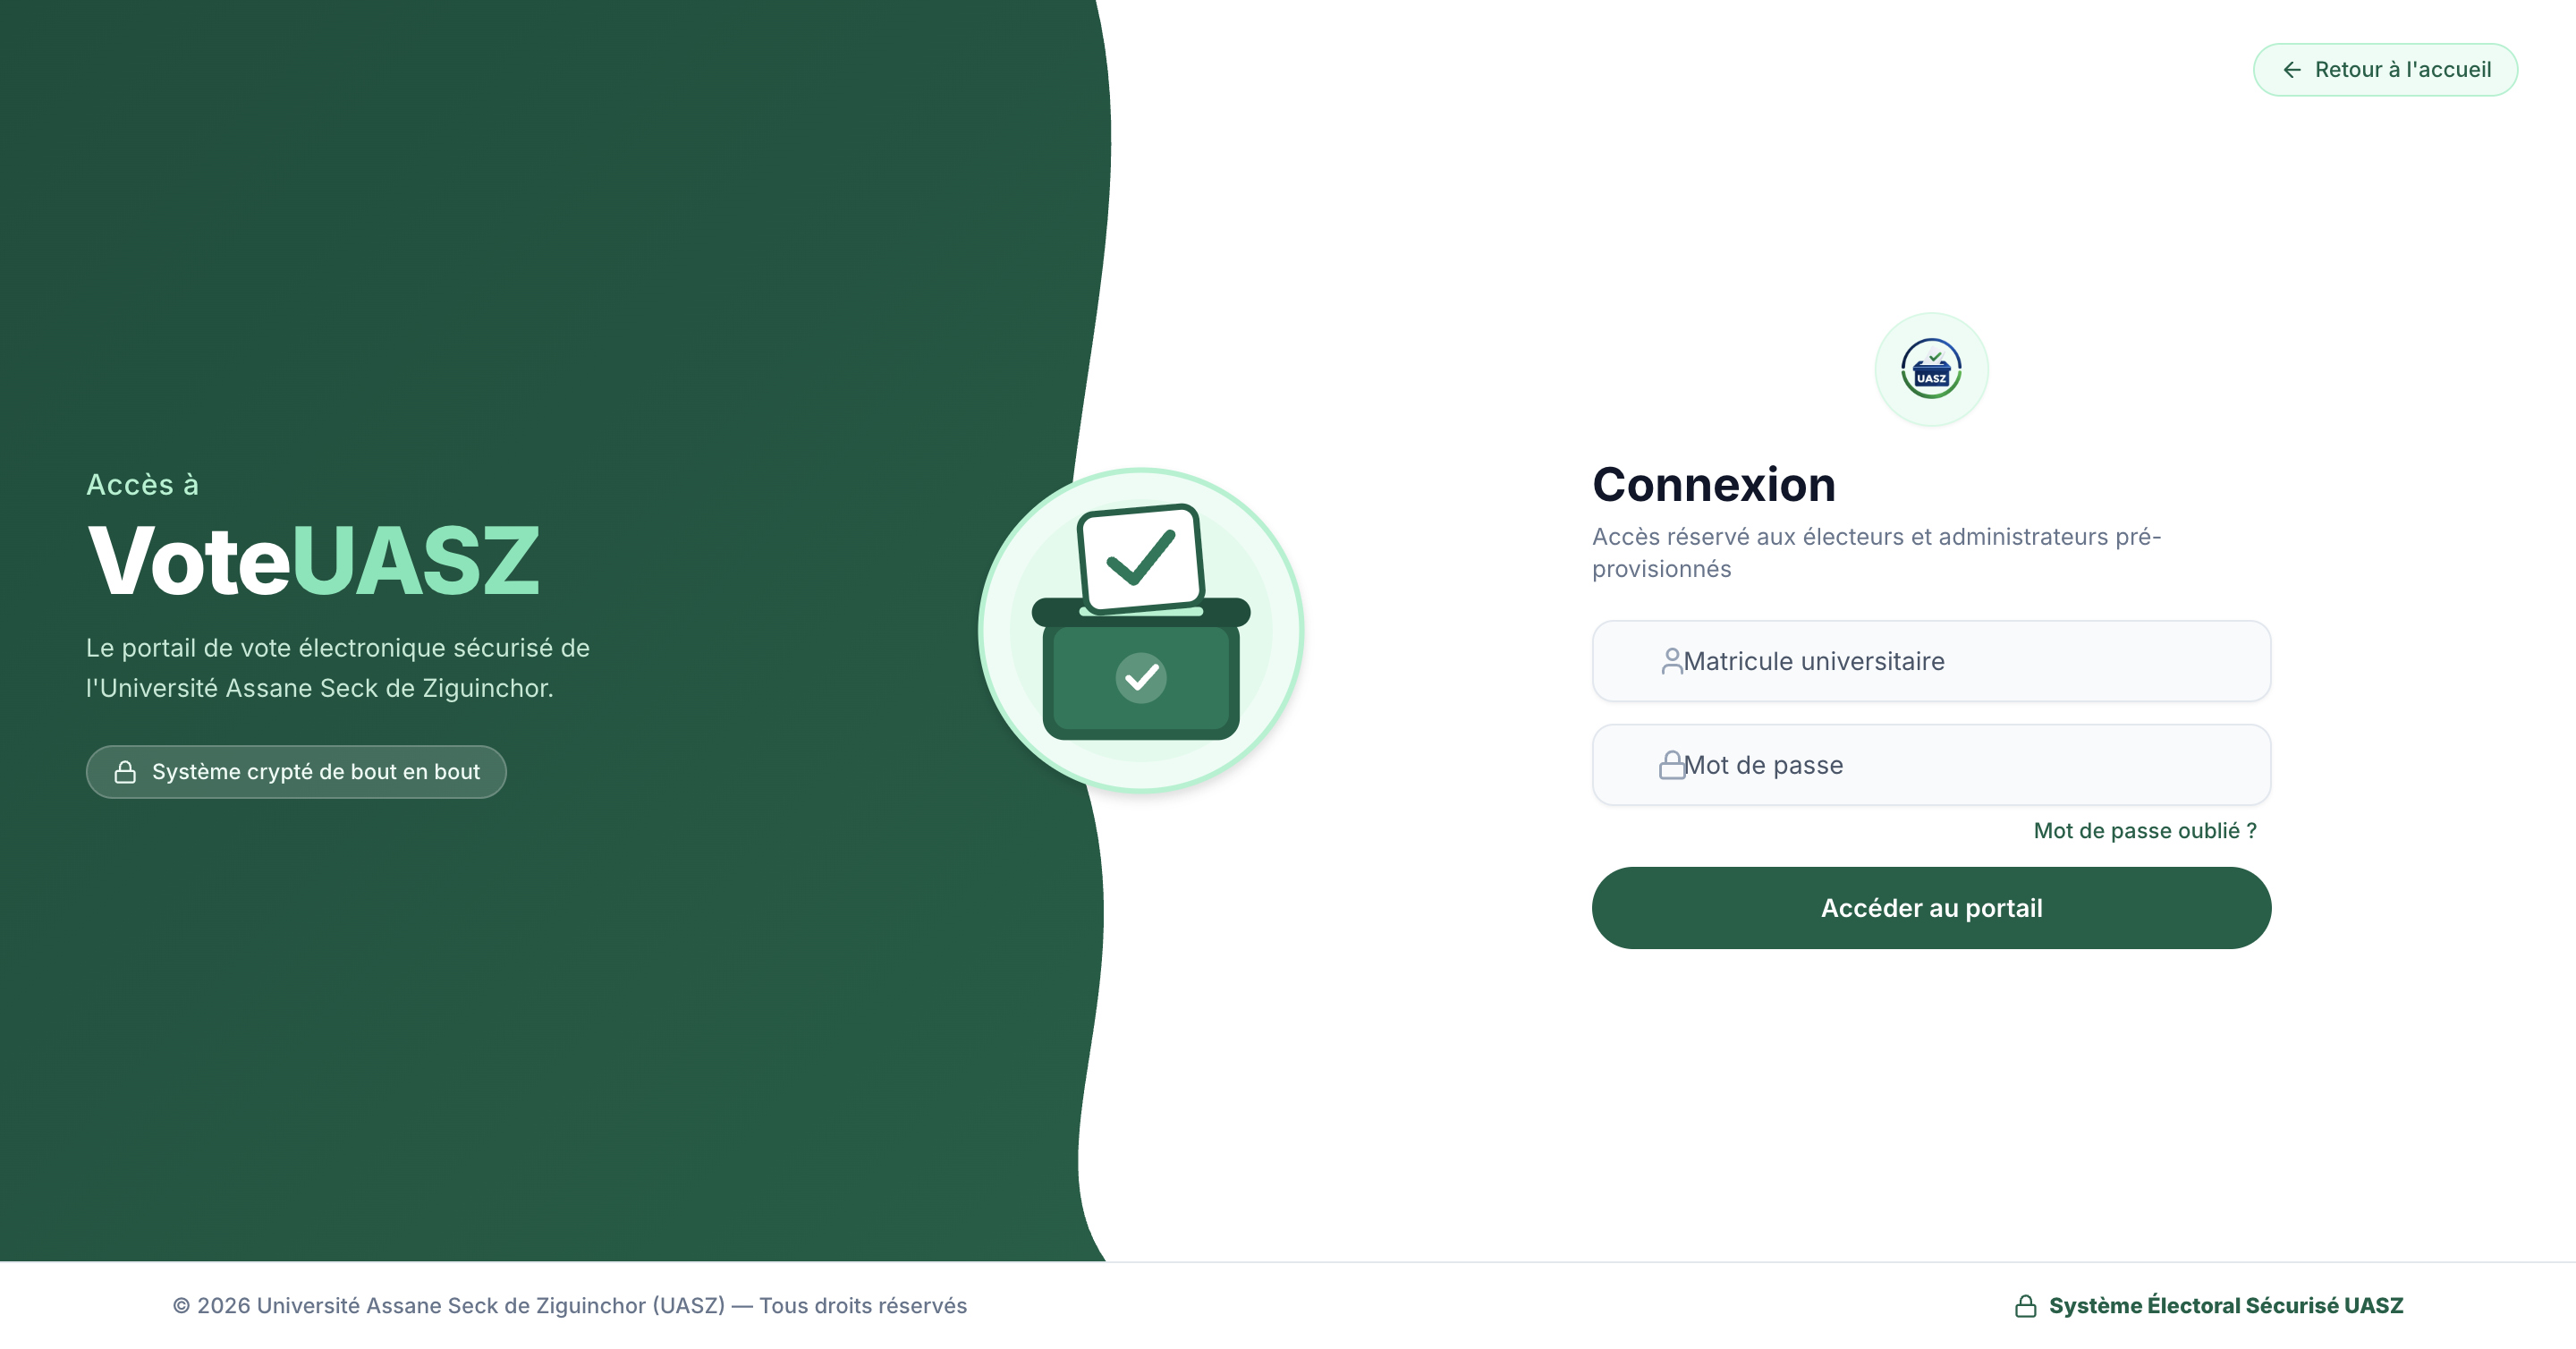
\includegraphics[width=0.88\textwidth,height=0.45\textheight,keepaspectratio]{3-2-1-login-desktop.png}
    \caption{Page de connexion compacte en mode desktop (\texttt{1440x900})}
    \label{fig:login-desktop}
\end{figure}

\begin{figure}[H]
    \centering
    \begin{minipage}{0.38\textwidth}
        \centering
        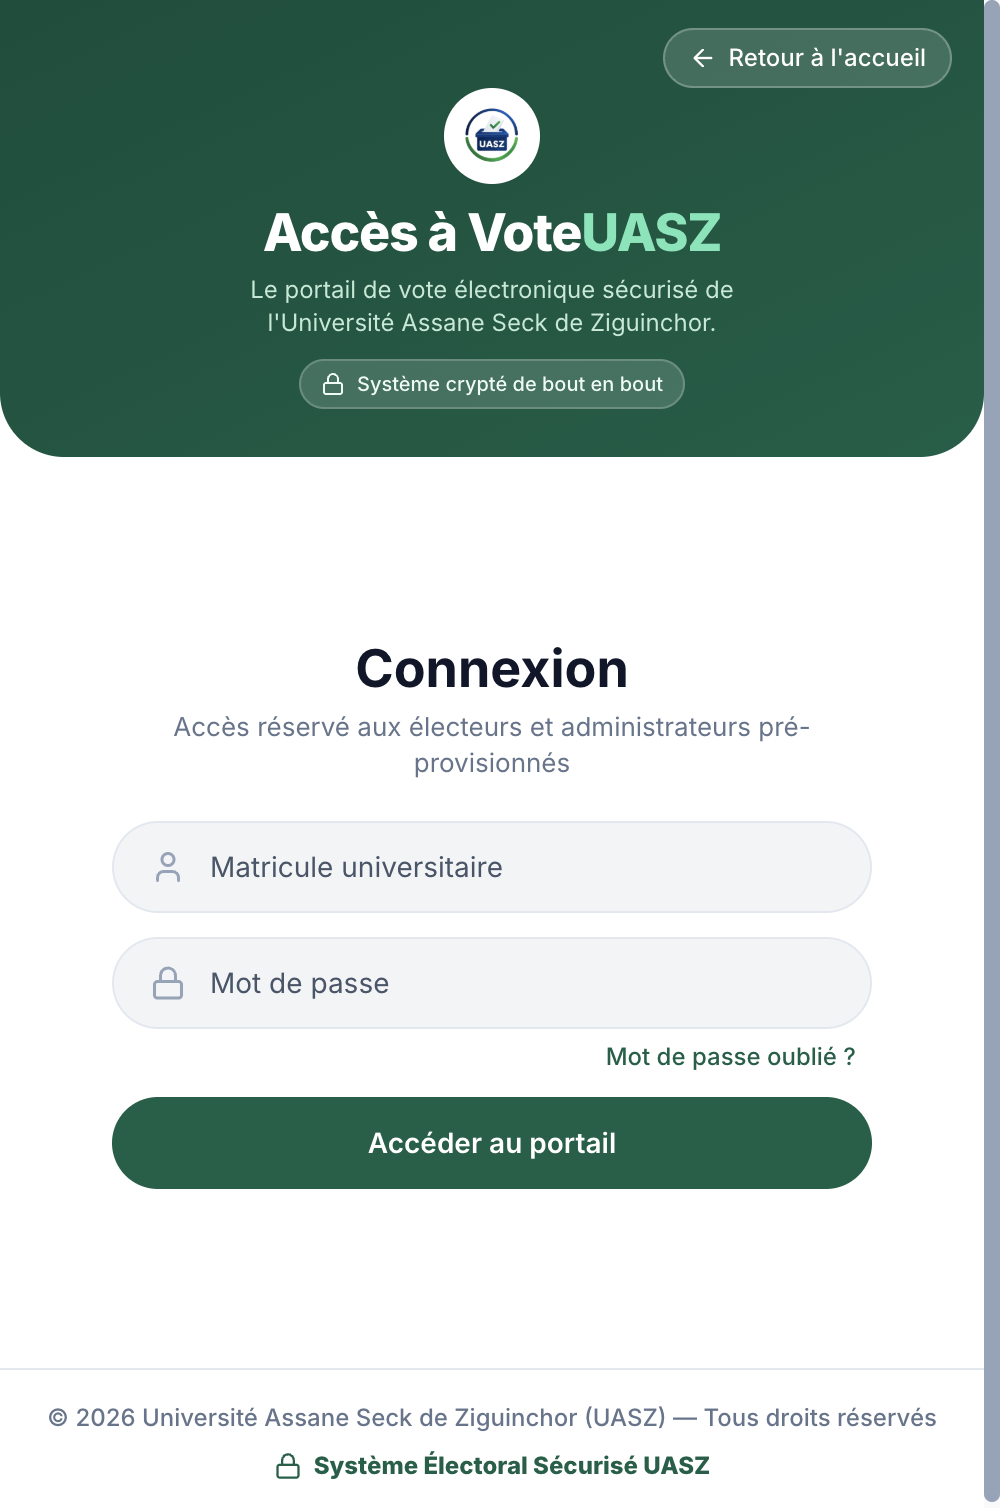
\includegraphics[width=\textwidth,height=0.42\textheight,keepaspectratio]{3-2-1-login-mobile.png}
        \caption{Connexion mobile (\texttt{390x844})}
        \label{fig:login-mobile}
    \end{minipage}
    \hfill
    \begin{minipage}{0.58\textwidth}
        \centering
        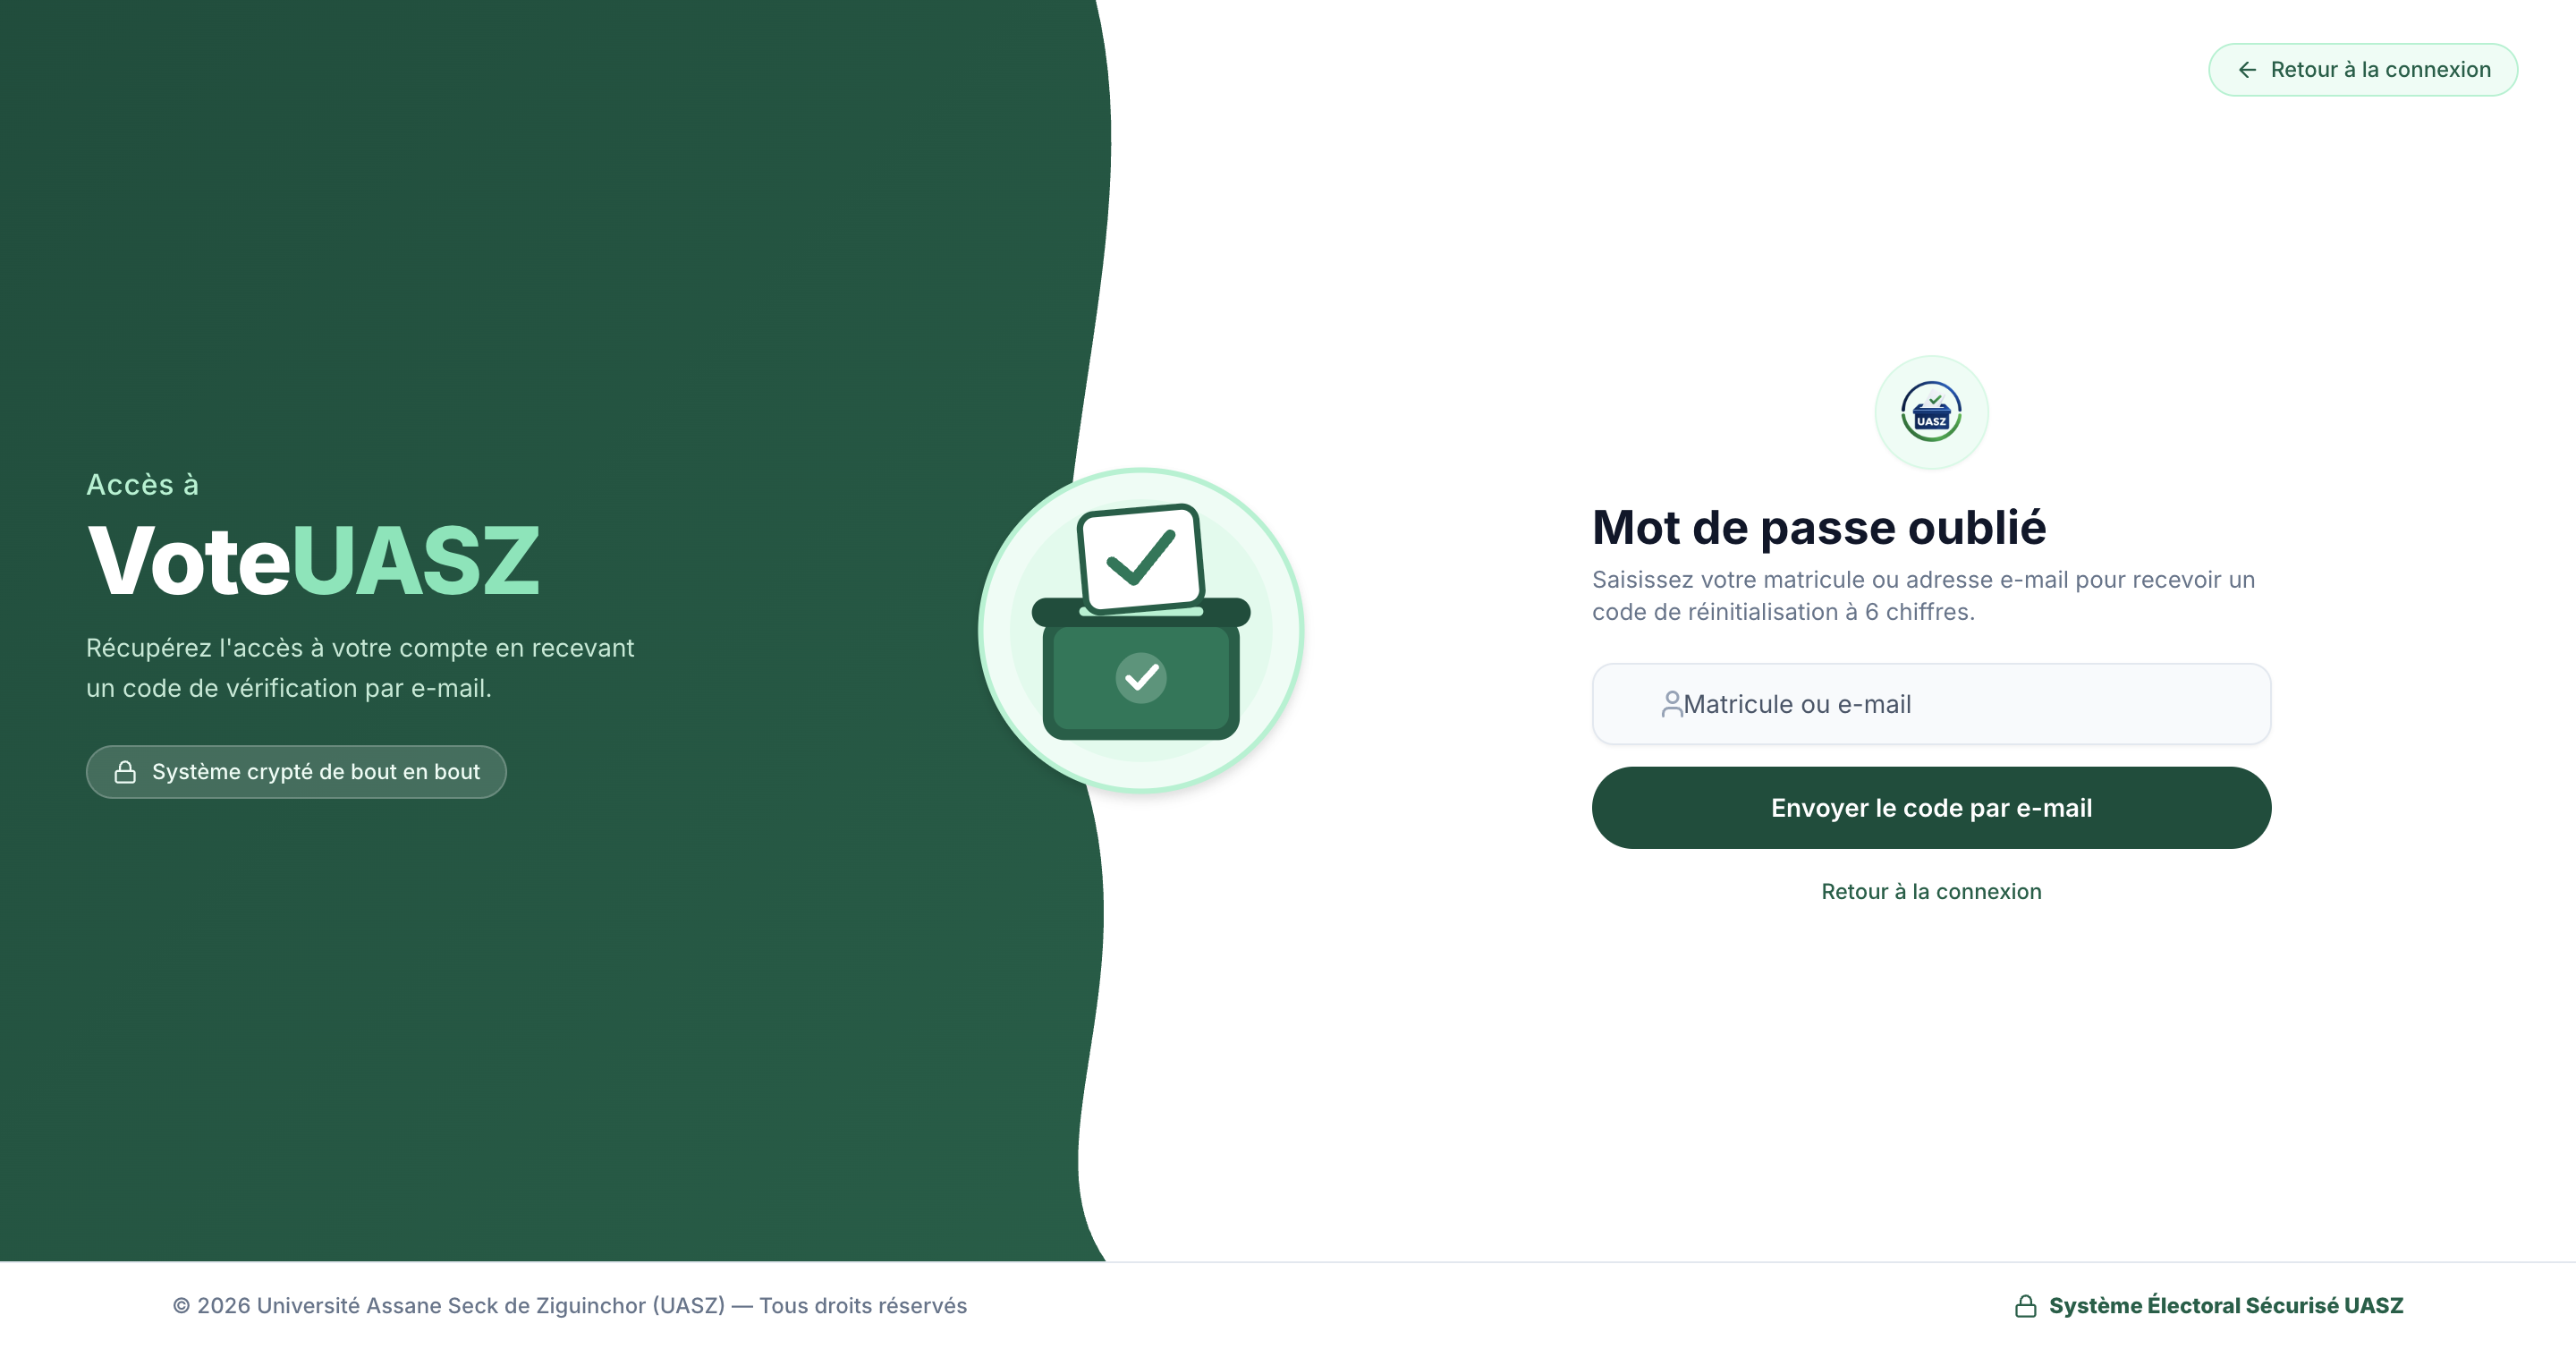
\includegraphics[width=\textwidth,height=0.42\textheight,keepaspectratio]{3-2-1-forgot-password.png}
        \caption{Demande de réinitialisation de mot de passe}
        \label{fig:forgot}
    \end{minipage}
\end{figure}

\begin{figure}[H]
    \centering
    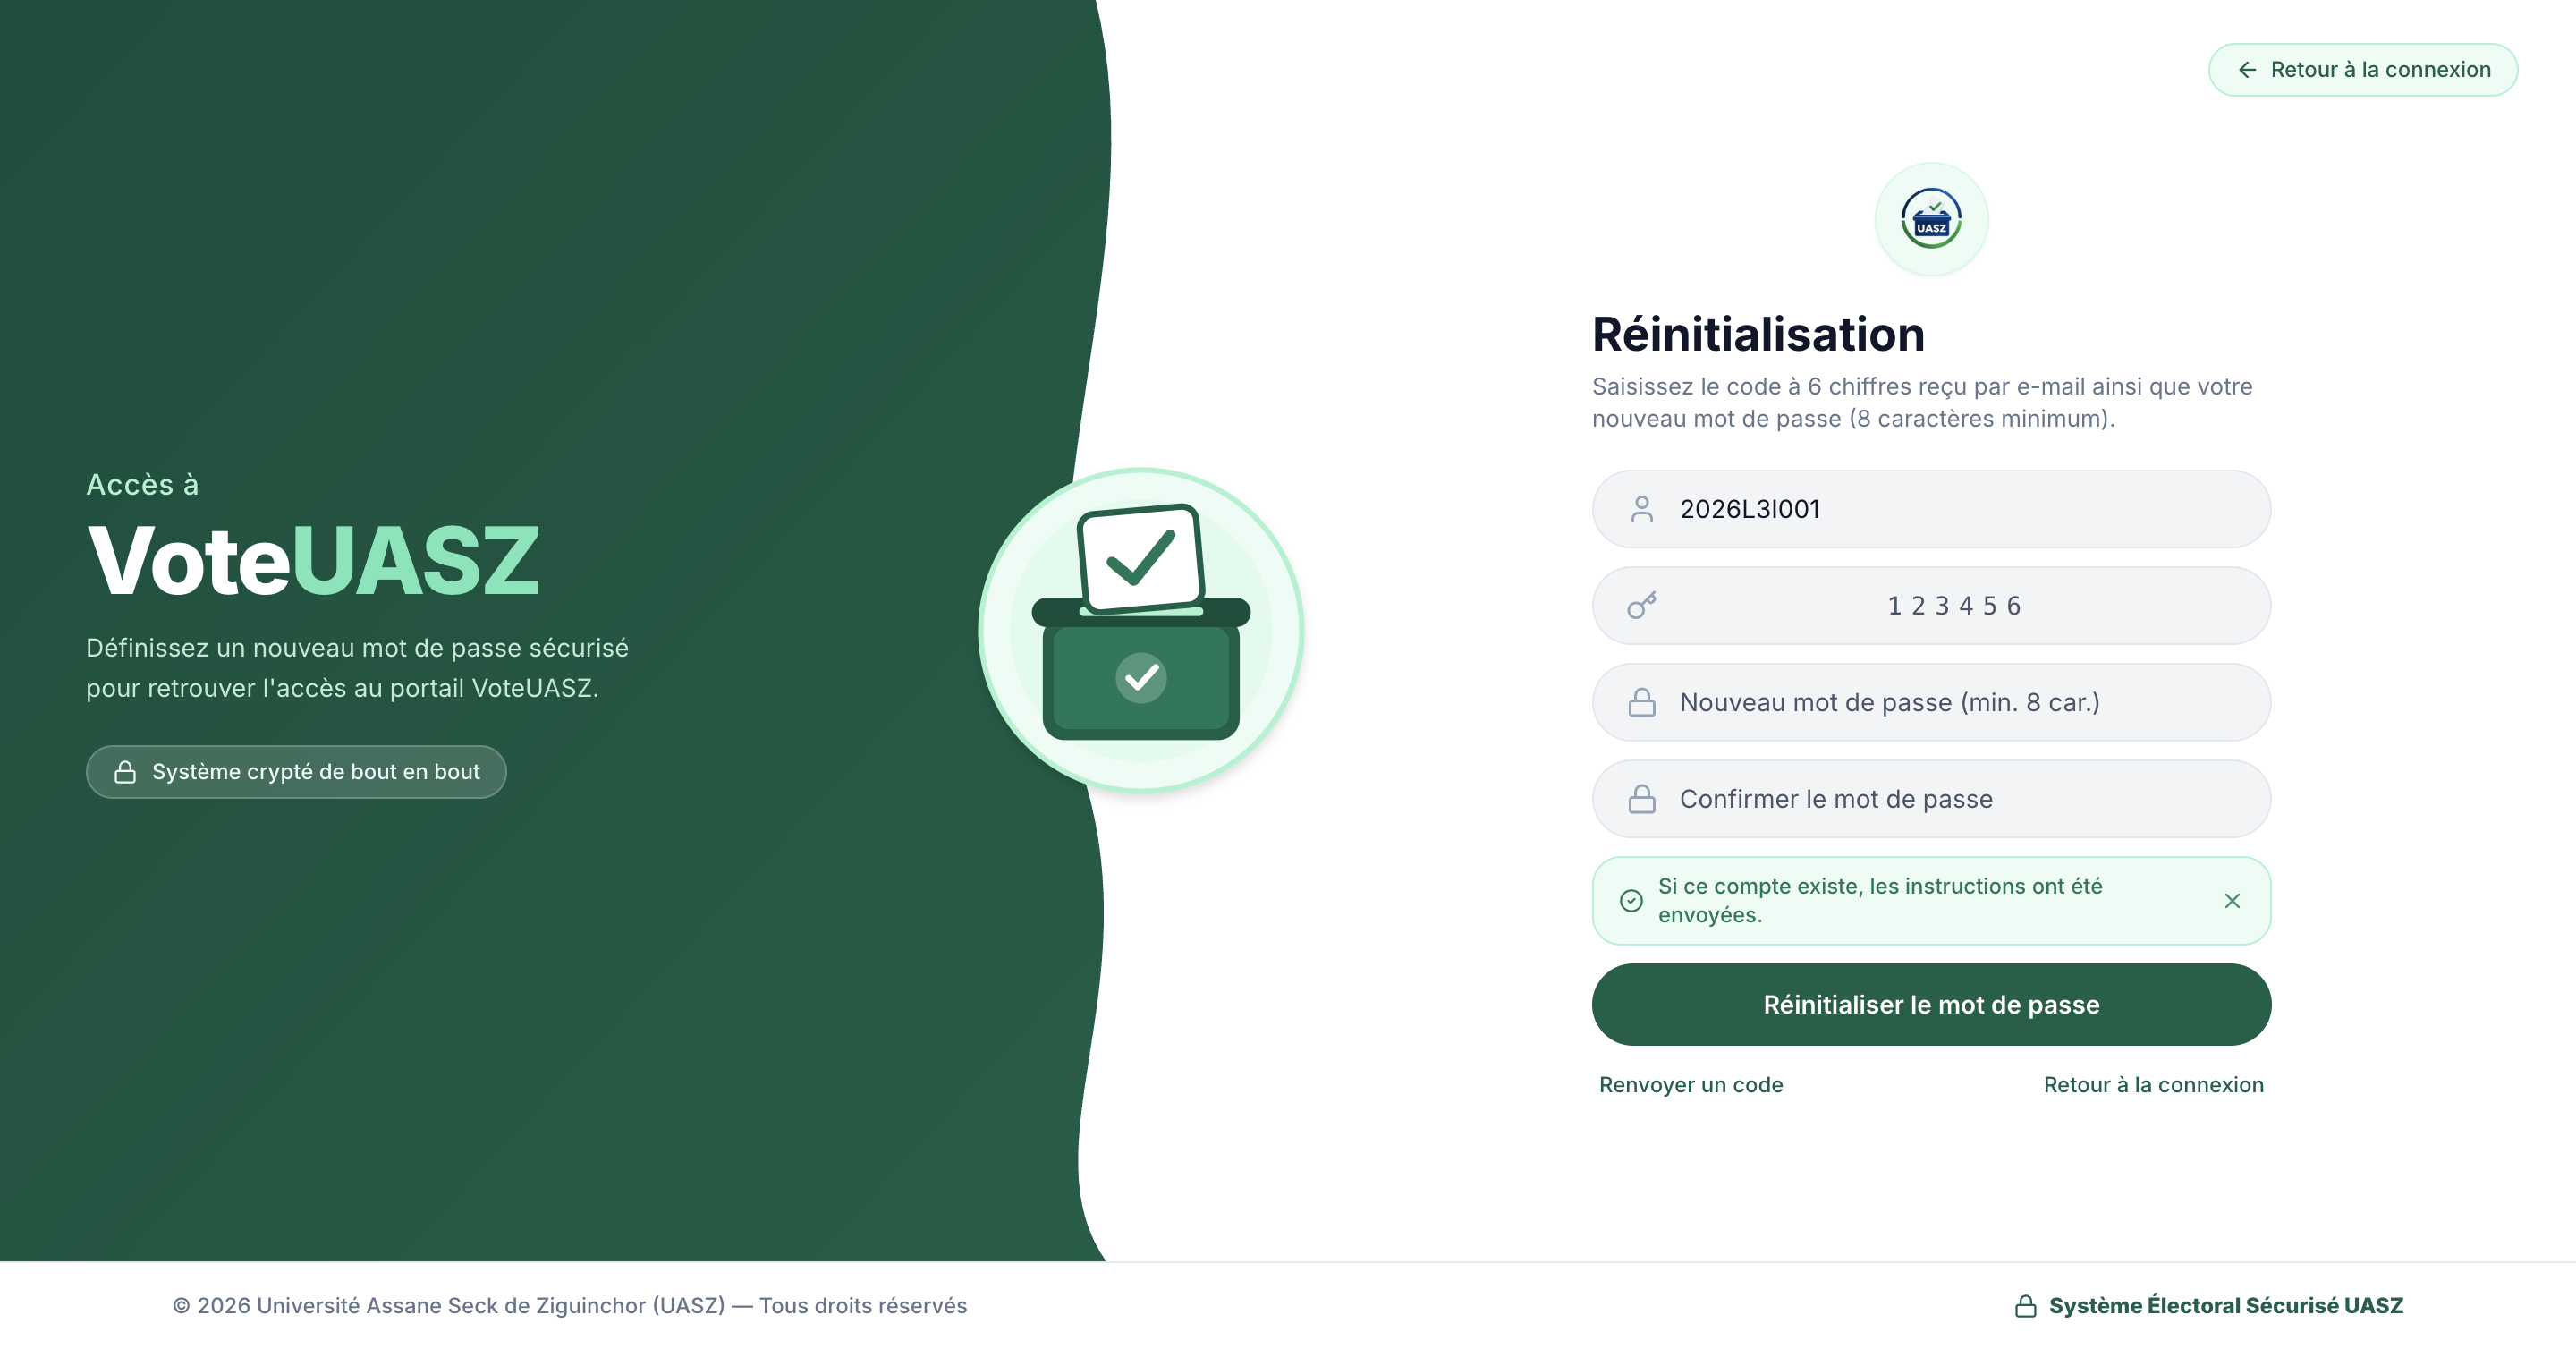
\includegraphics[width=0.85\textwidth,height=0.42\textheight,keepaspectratio]{3-2-1-reset-password.png}
    \caption{Saisie du code de réinitialisation et du nouveau mot de passe}
    \label{fig:reset}
\end{figure}

\subsection{Consultation des scrutins et vote sécurisé}
Les figures~\ref{fig:elec-tab}, \ref{fig:elec-cards} et~\ref{fig:elec-mob} présentent la liste des 5 scrutins (vues tableau, cartes et mobile). Les figures~\ref{fig:detail-stepper}, \ref{fig:detail-otp}, \ref{fig:mailhog-otp}, \ref{fig:detail-drawer}, \ref{fig:detail-results} et~\ref{fig:detail-mobile} montrent le stepper de vote en 3 étapes, l'e-mail OTP reçu dans MailHog, le drawer de campagne (photo, affiche, vidéo YouTube et texte long) et le graphique Chart.js des résultats en direct.

\begin{figure}[H]
    \centering
    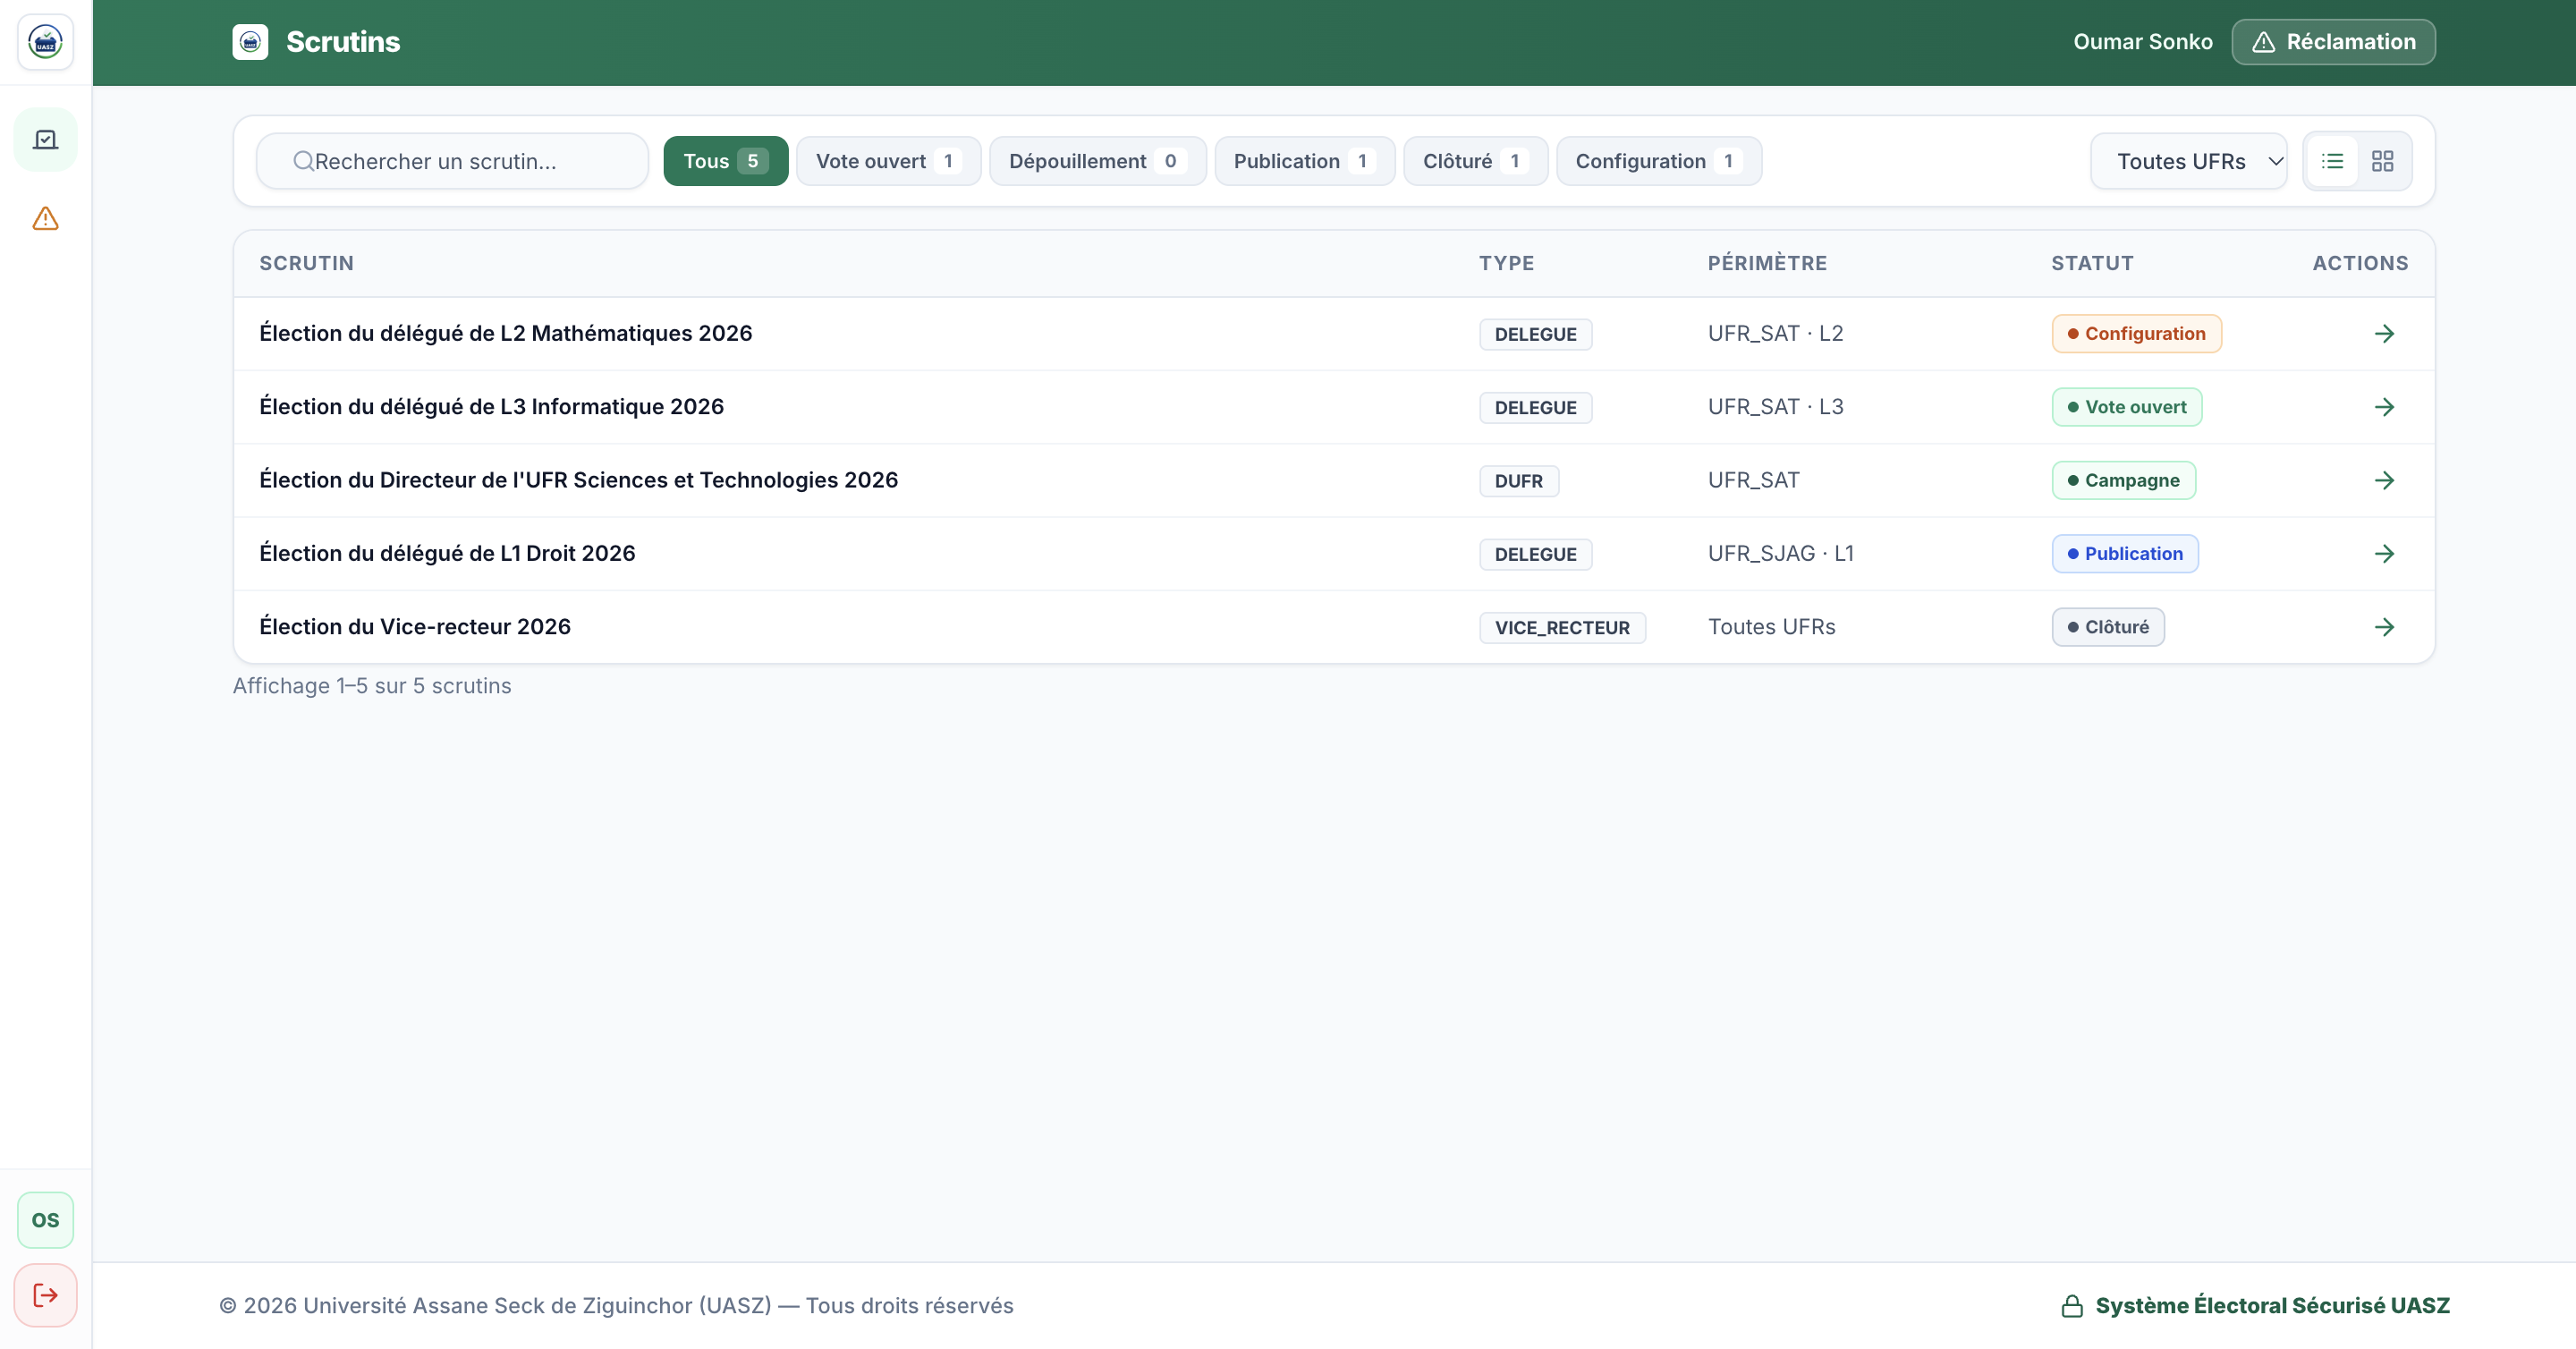
\includegraphics[width=0.92\textwidth,height=0.44\textheight,keepaspectratio]{3-2-2-elections-tableau.png}
    \caption{Liste des scrutins en vue tableau (\texttt{/elections})}
    \label{fig:elec-tab}
\end{figure}

\begin{figure}[H]
    \centering
    \begin{minipage}{0.62\textwidth}
        \centering
        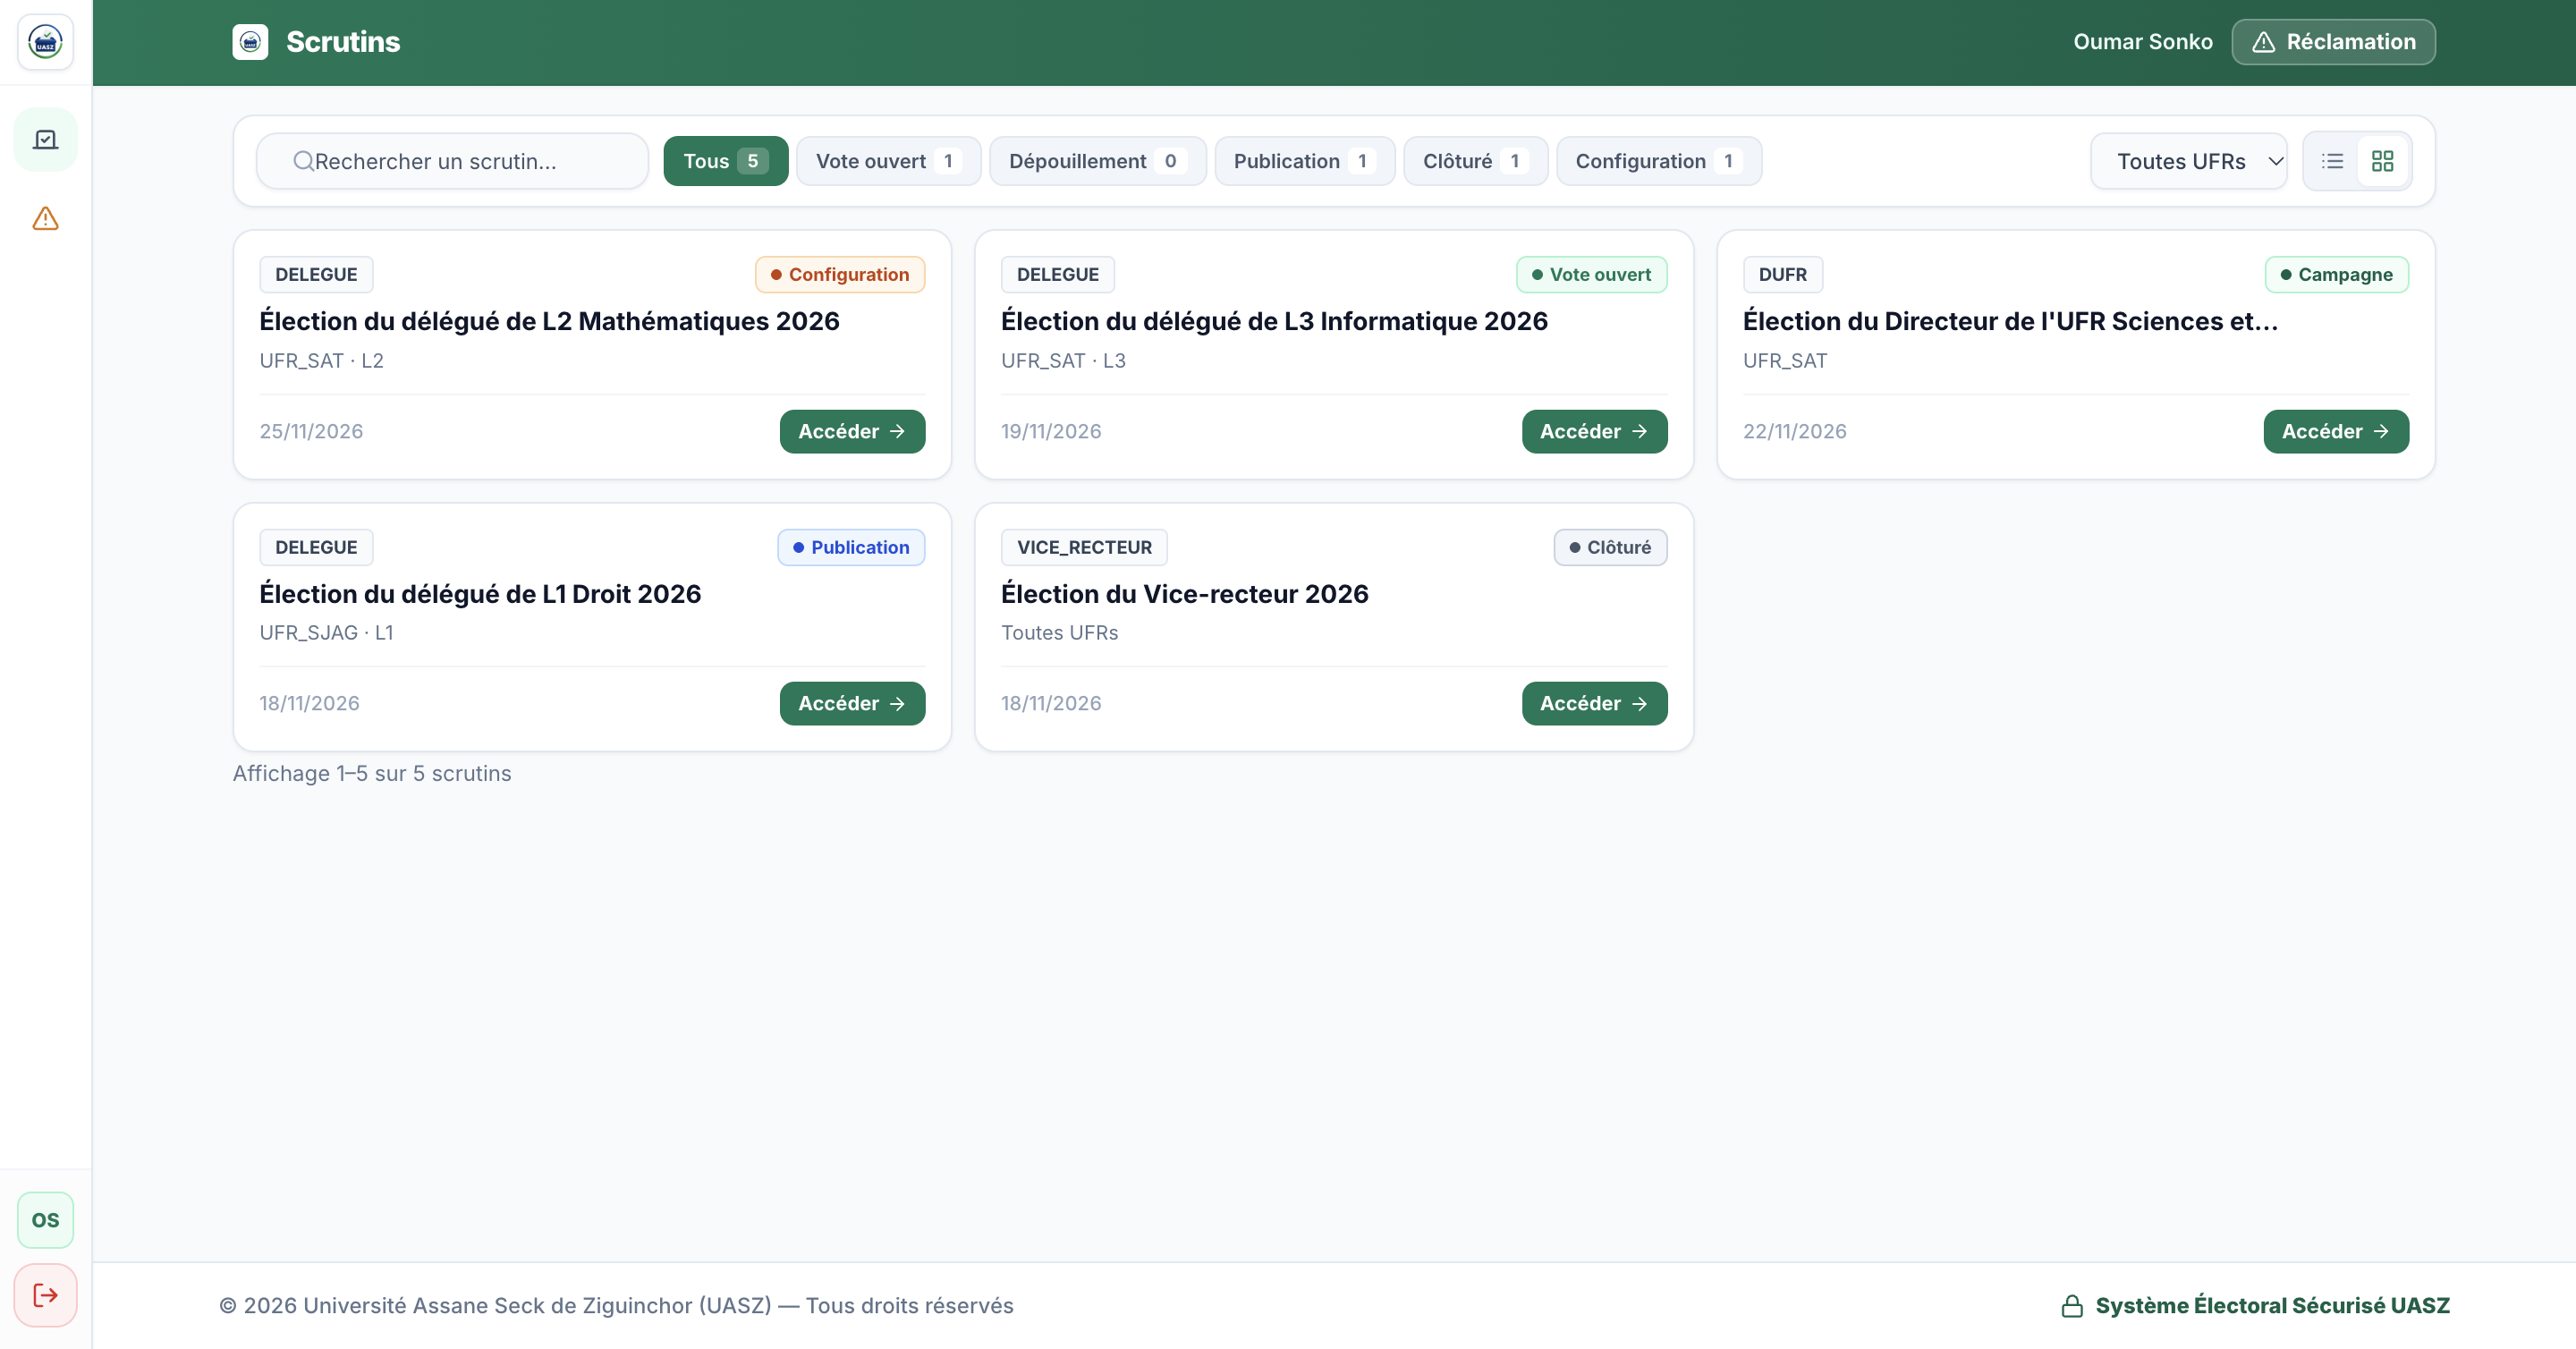
\includegraphics[width=\textwidth,height=0.42\textheight,keepaspectratio]{3-2-2-elections-cartes.png}
        \caption{Liste des scrutins en vue cartes}
        \label{fig:elec-cards}
    \end{minipage}
    \hfill
    \begin{minipage}{0.34\textwidth}
        \centering
        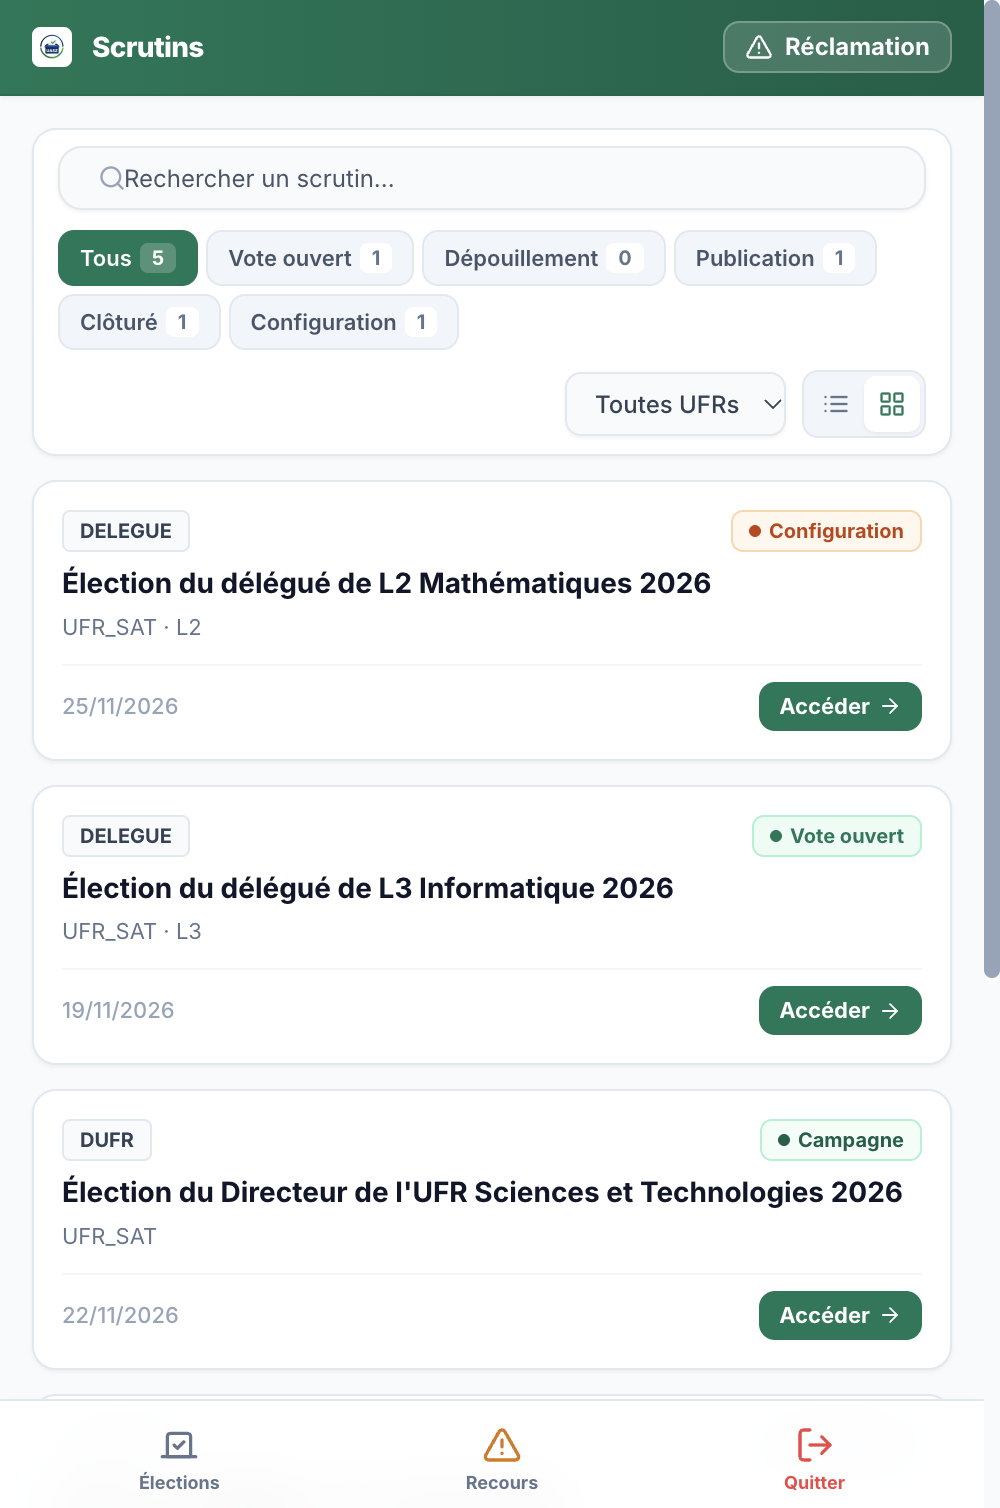
\includegraphics[width=\textwidth,height=0.42\textheight,keepaspectratio]{3-2-2-elections-mobile.png}
        \caption{Vue mobile (\texttt{390x844})}
        \label{fig:elec-mob}
    \end{minipage}
\end{figure}

\begin{figure}[H]
    \centering
    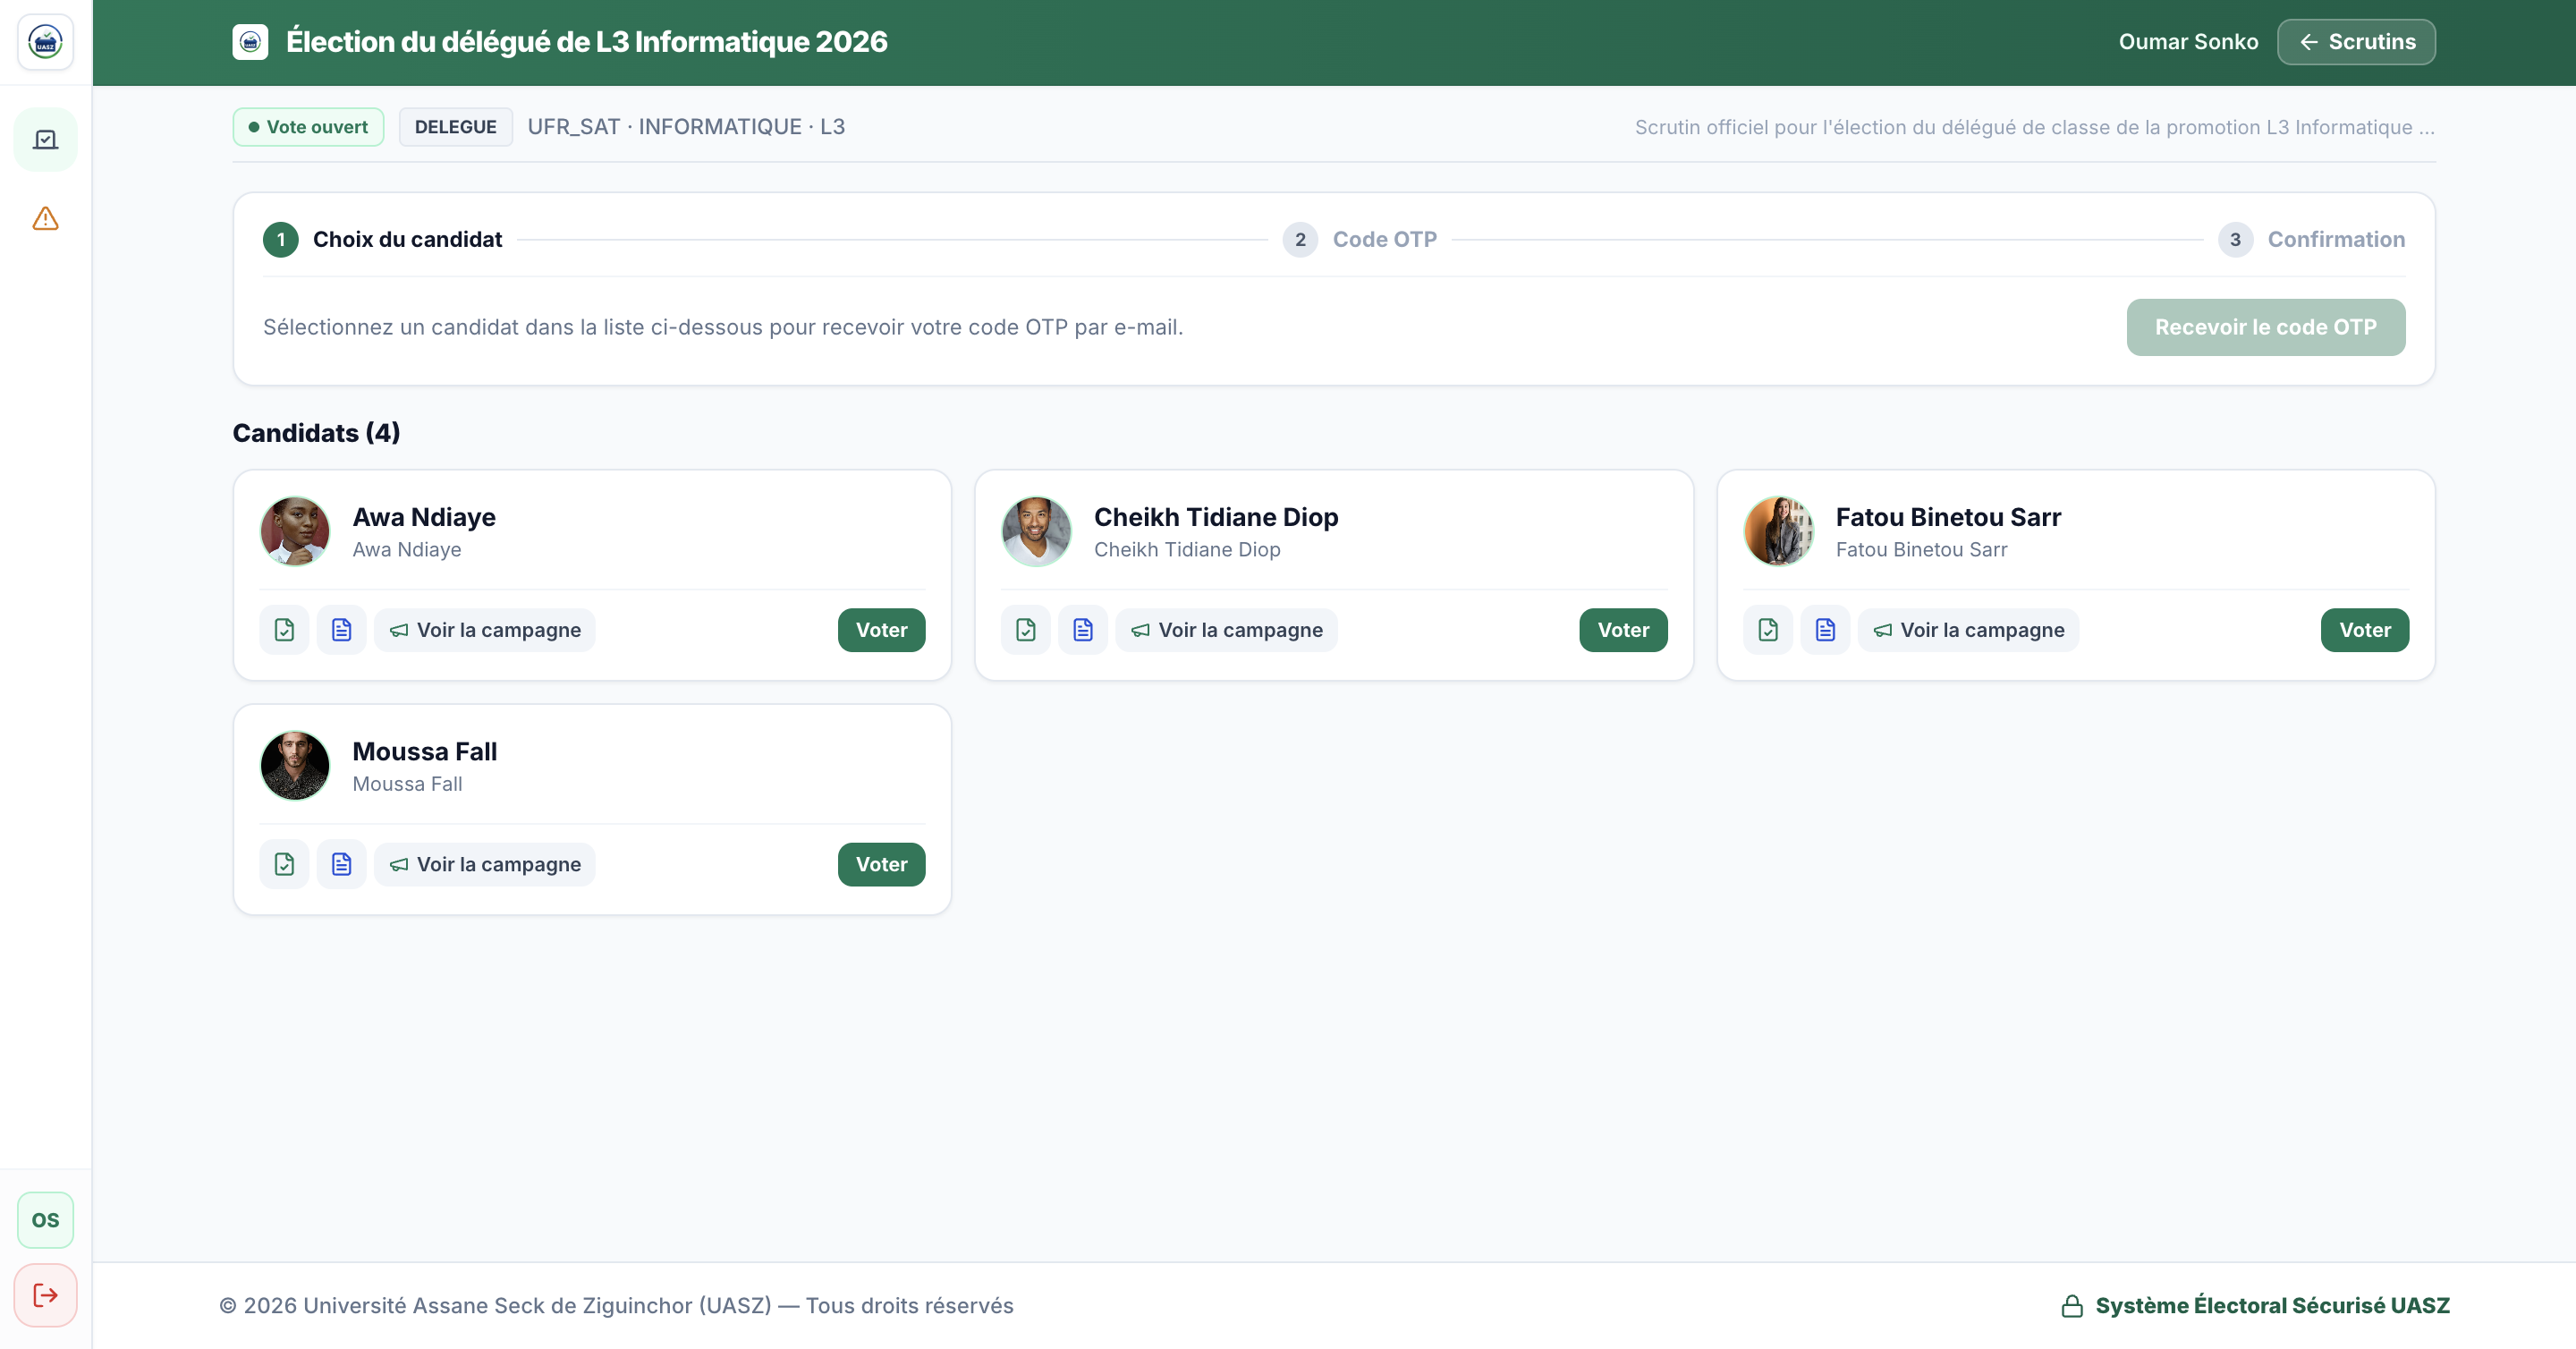
\includegraphics[width=0.92\textwidth,height=0.44\textheight,keepaspectratio]{3-2-3-election-detail-stepper.png}
    \caption{Détail d'élection ouverte : stepper de vote en 3 étapes (\texttt{L3 Informatique 2026})}
    \label{fig:detail-stepper}
\end{figure}

\begin{figure}[H]
    \centering
    \begin{minipage}{0.48\textwidth}
        \centering
        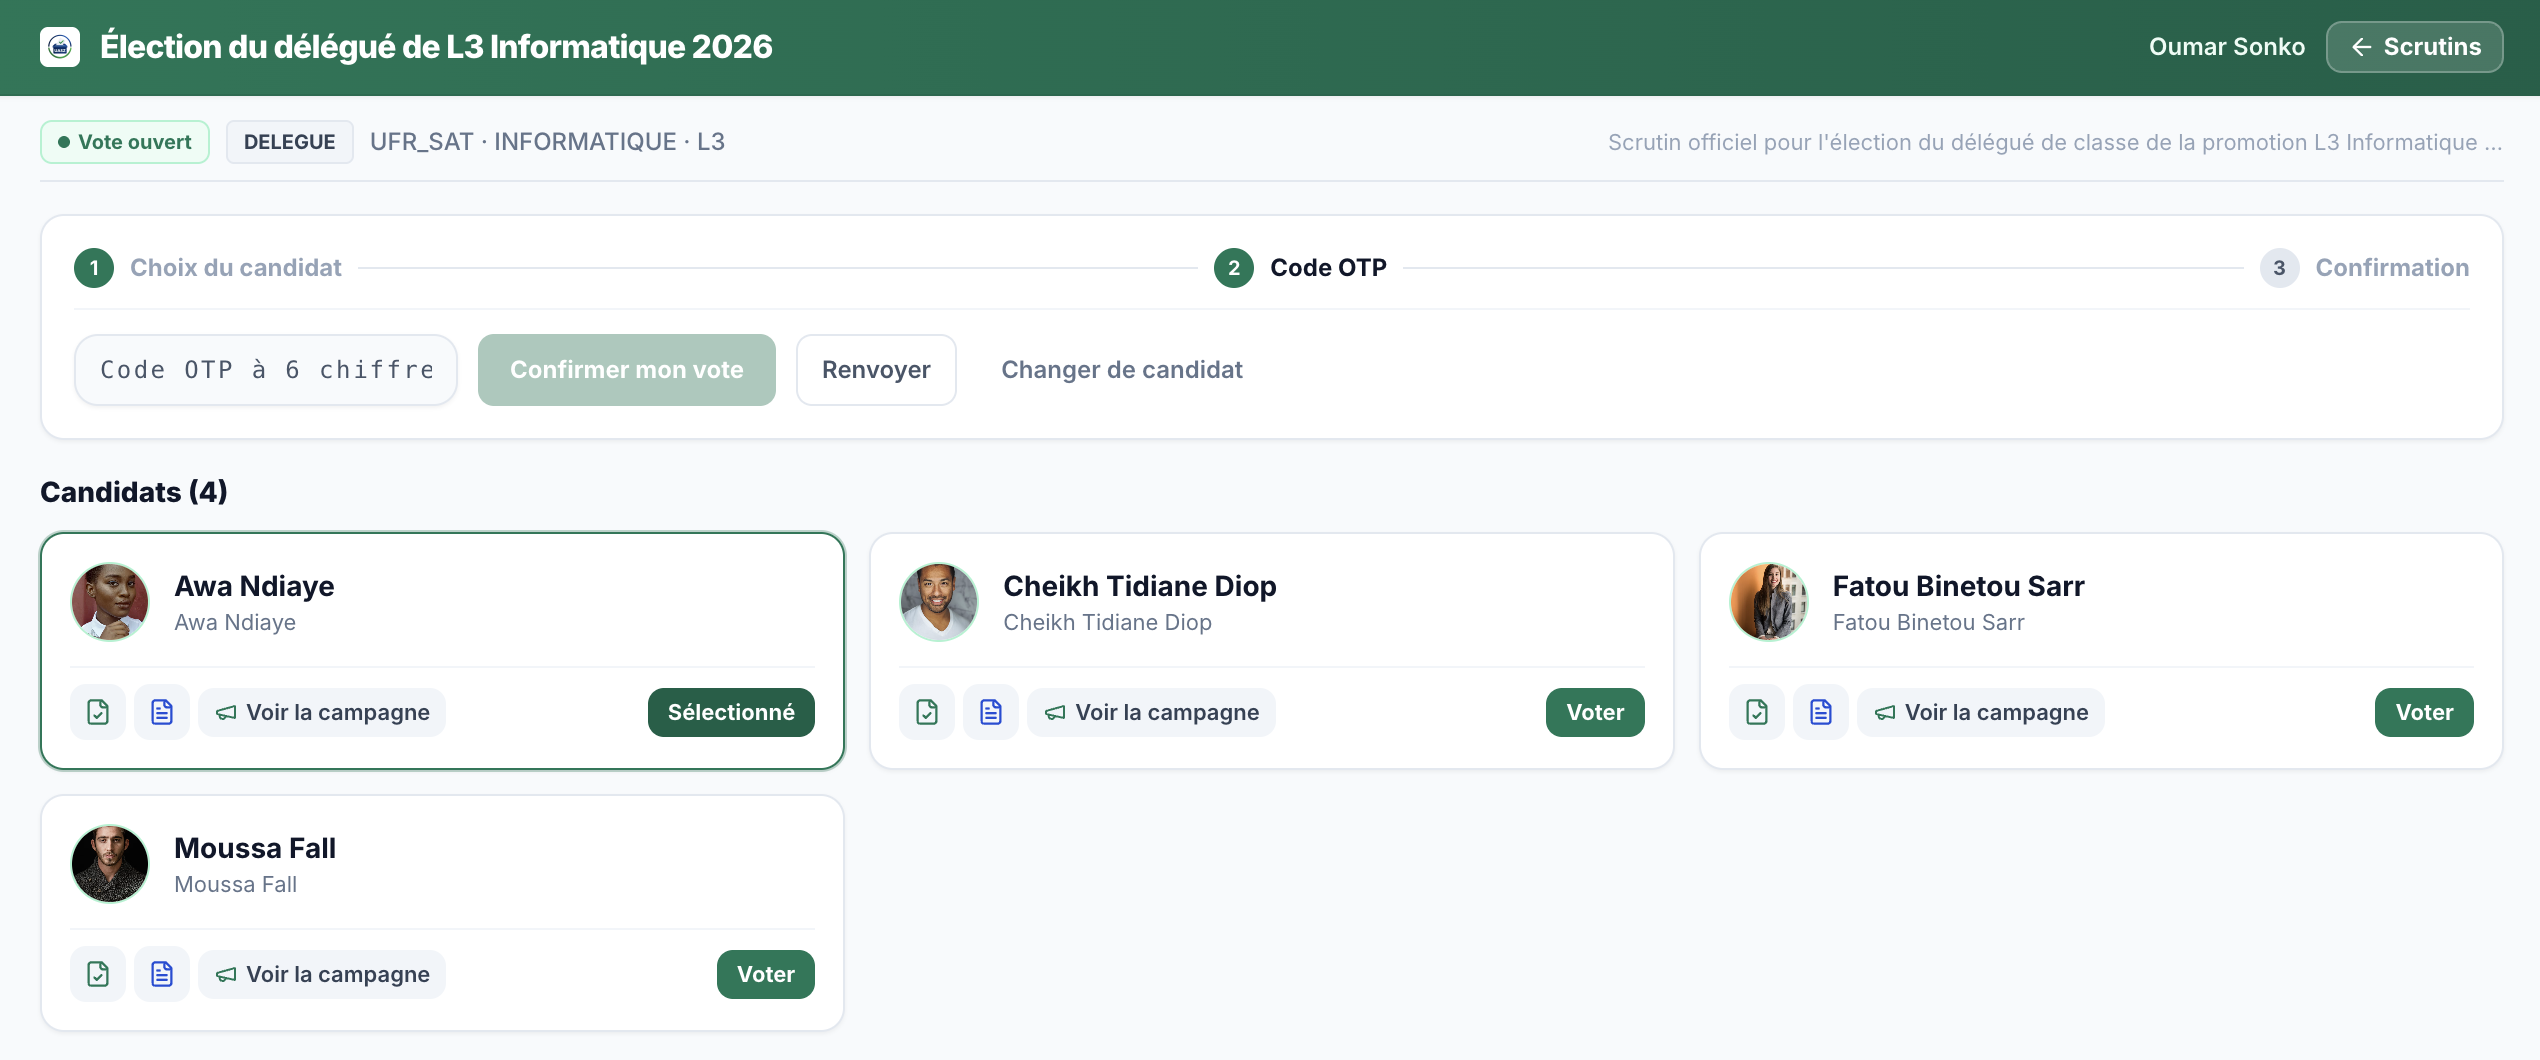
\includegraphics[width=\textwidth,height=0.38\textheight,keepaspectratio]{3-2-3-election-detail-otp.png}
        \caption{Étape de saisie du code OTP}
        \label{fig:detail-otp}
    \end{minipage}
    \hfill
    \begin{minipage}{0.48\textwidth}
        \centering
        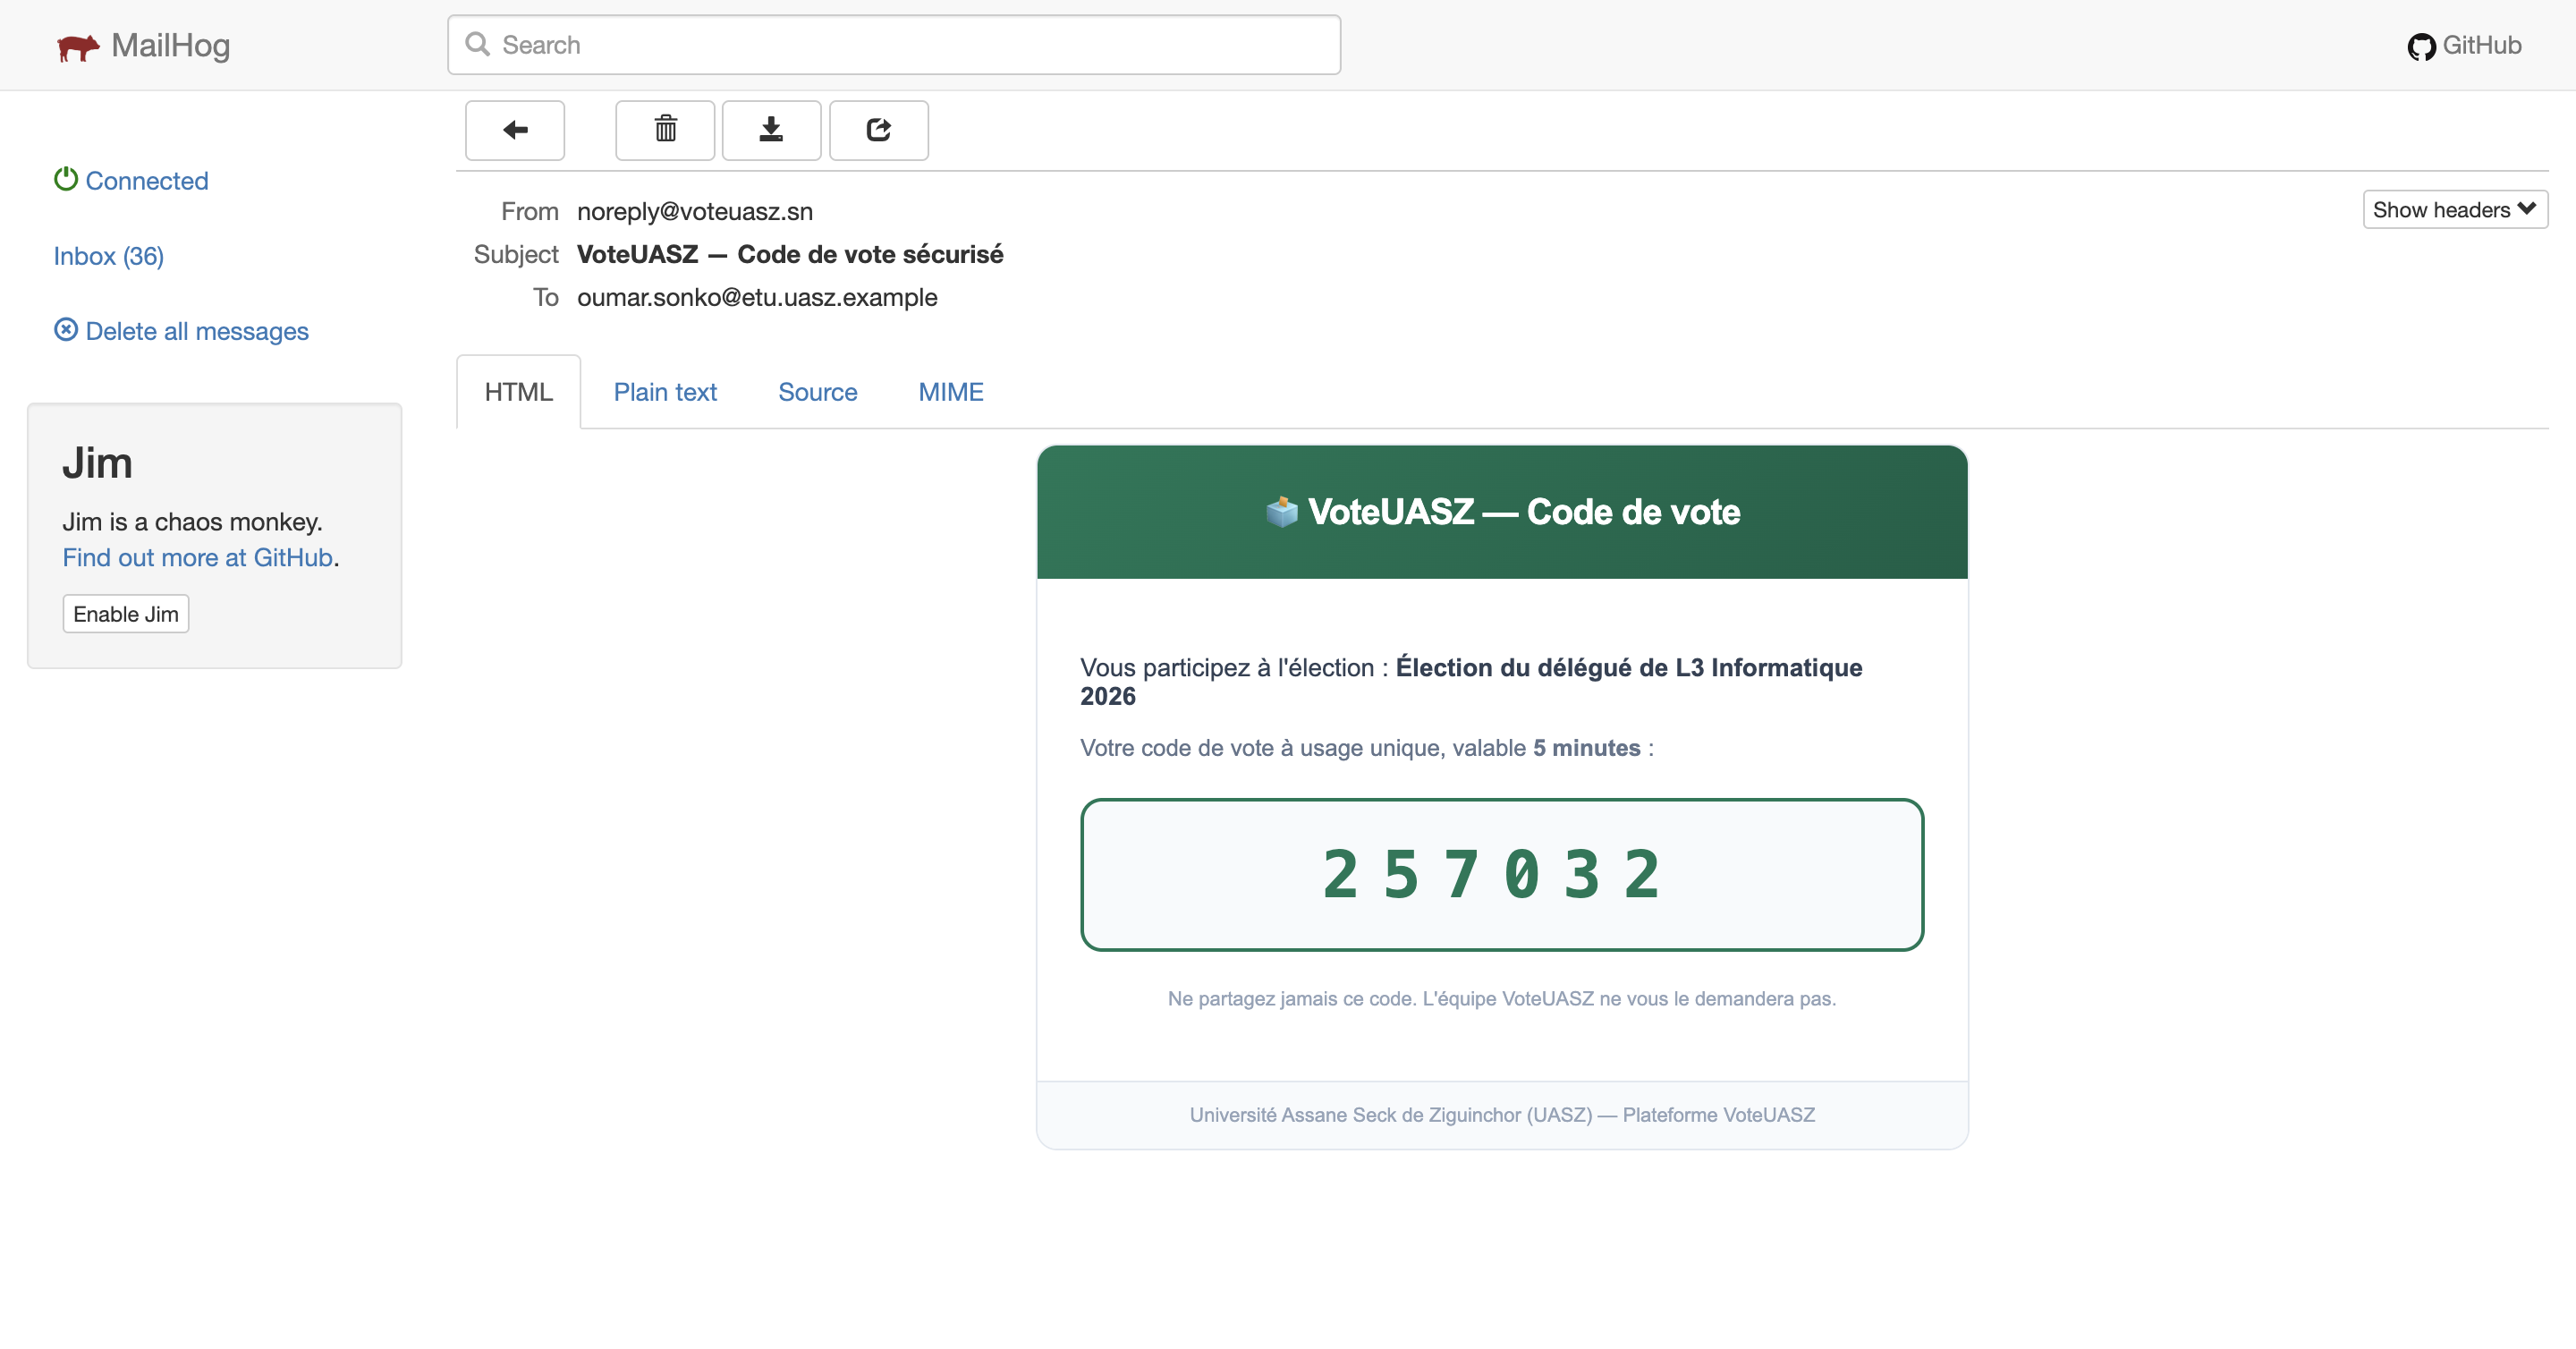
\includegraphics[width=\textwidth,height=0.38\textheight,keepaspectratio]{3-2-4-mailhog-otp.png}
        \caption{E-mail OTP reçu dans MailHog}
        \label{fig:mailhog-otp}
    \end{minipage}
\end{figure}

\begin{figure}[H]
    \centering
    \begin{minipage}{0.62\textwidth}
        \centering
        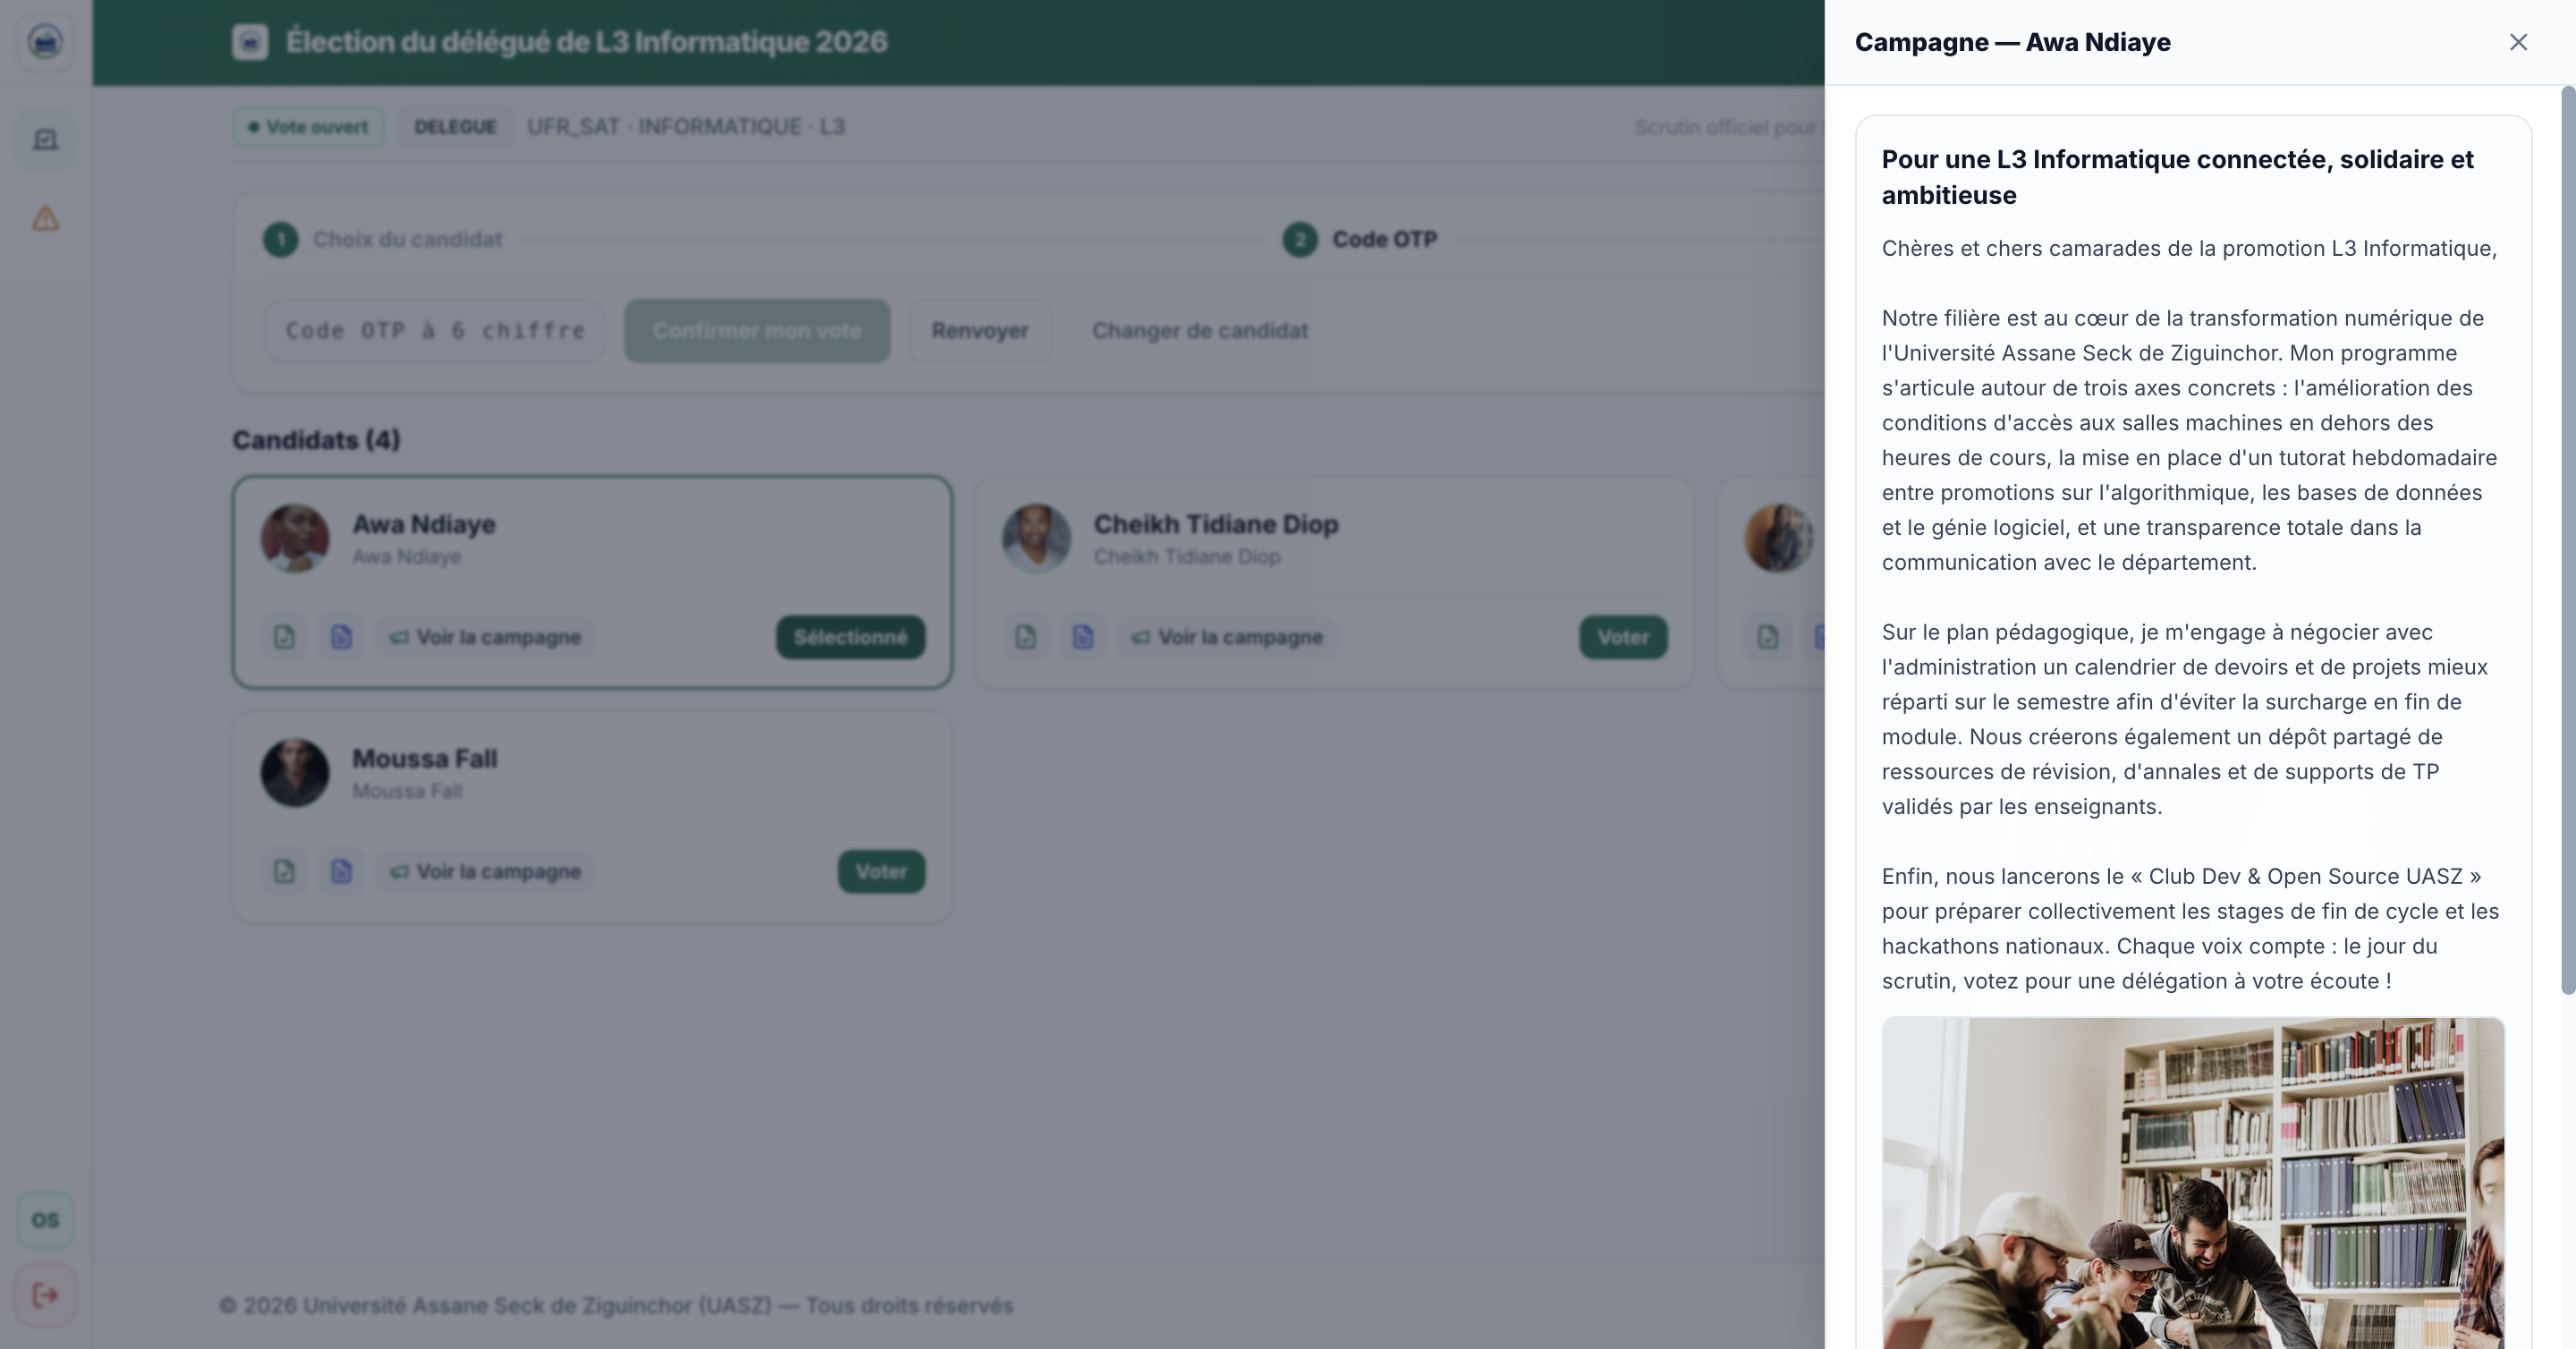
\includegraphics[width=\textwidth,height=0.42\textheight,keepaspectratio]{3-2-3-election-detail-drawer.png}
        \caption{Drawer de campagne (photo, affiche, vidéo YouTube et programme)}
        \label{fig:detail-drawer}
    \end{minipage}
    \hfill
    \begin{minipage}{0.34\textwidth}
        \centering
        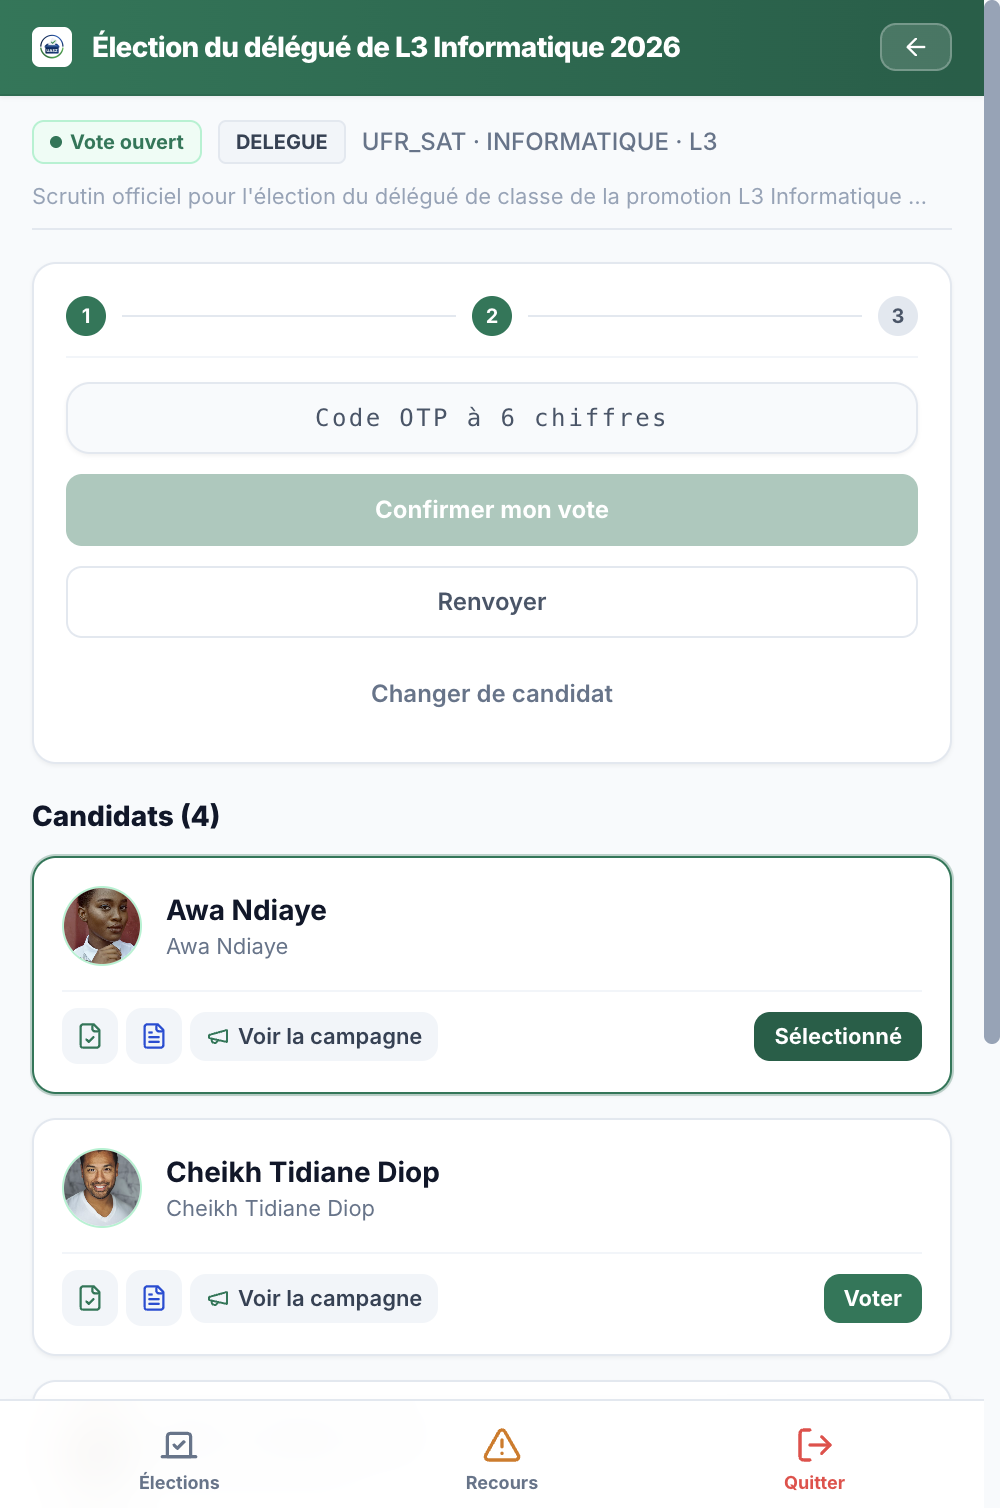
\includegraphics[width=\textwidth,height=0.42\textheight,keepaspectratio]{3-2-3-election-detail-mobile.png}
        \caption{Détail mobile (\texttt{390x844})}
        \label{fig:detail-mobile}
    \end{minipage}
\end{figure}

\begin{figure}[H]
    \centering
    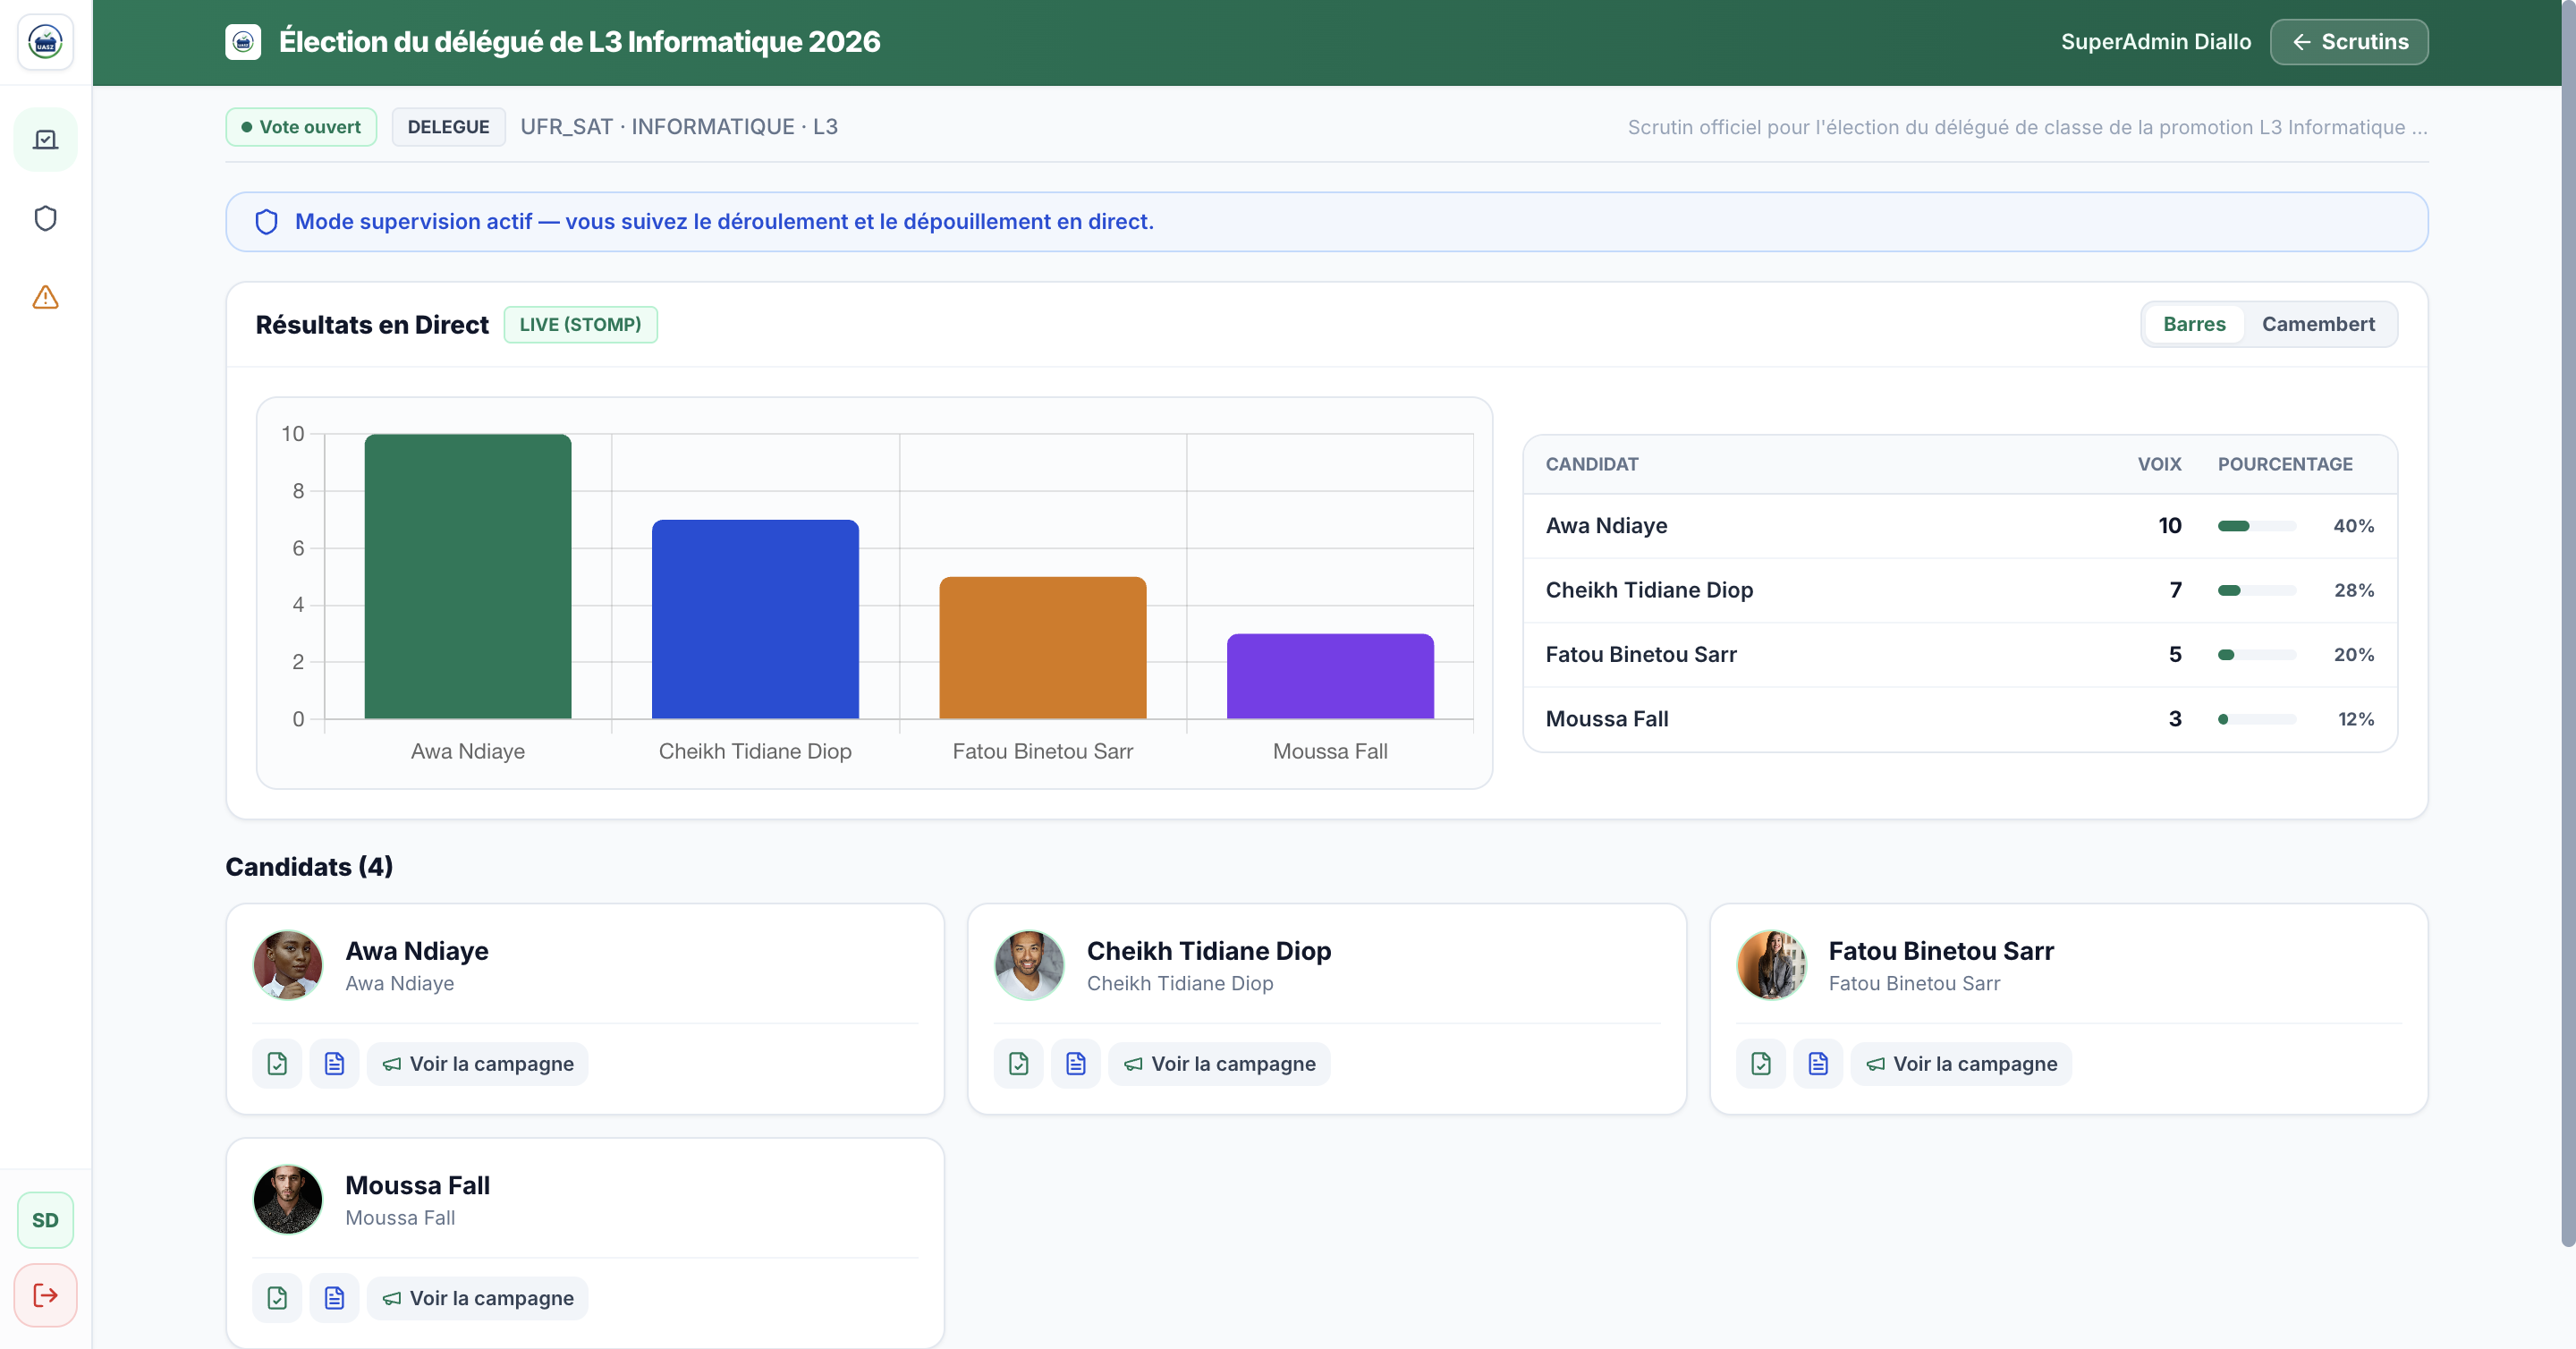
\includegraphics[width=0.92\textwidth,height=0.44\textheight,keepaspectratio]{3-2-3-election-detail-results-live.png}
    \caption{Résultats en direct à 4 candidats avec graphique Chart.js affiché automatiquement}
    \label{fig:detail-results}
\end{figure}

\subsection{Administration, Commission, Candidat, Réclamations et PV PDF}
Les figures~\ref{fig:admin-scrutins} à~\ref{fig:swagger} présentent l'espace Super-Admin (scrutins, drawer de création, import CSV, audit SHA-256), l'espace Commission (validation/rejet motivé et réclamations), l'espace Candidat, les réclamations électeur (desktop/mobile), le PV PDF généré et la documentation Swagger UI locale.

\begin{figure}[H]
    \centering
    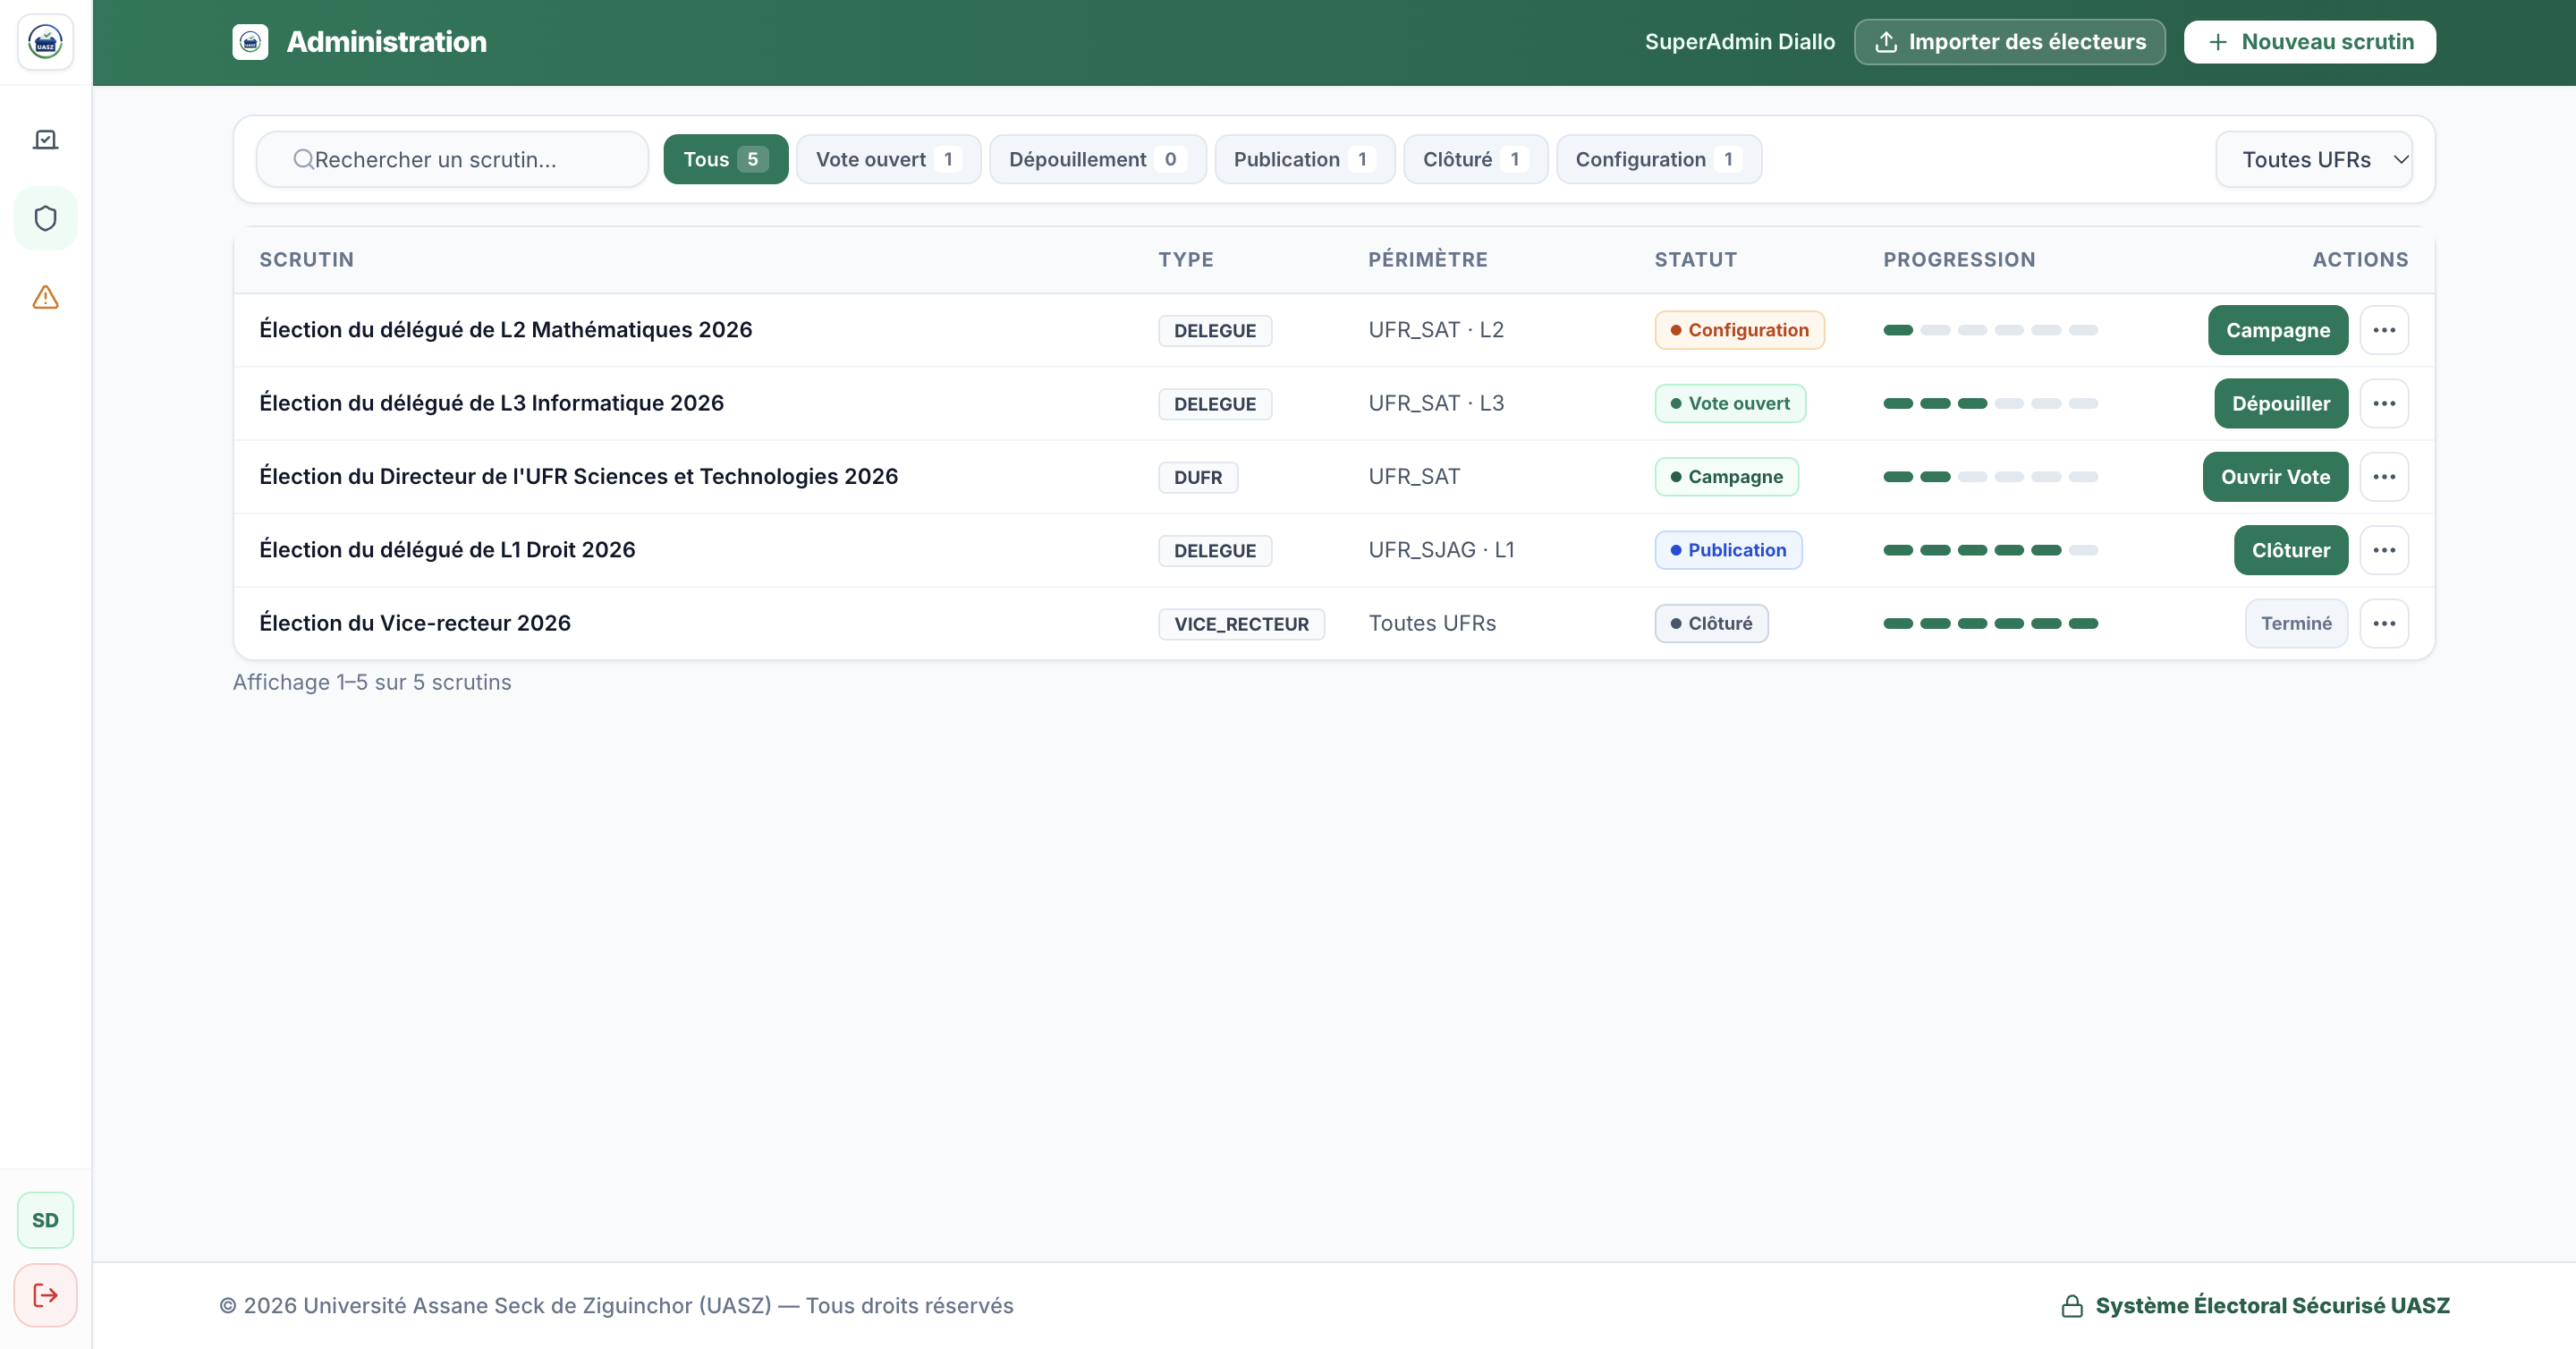
\includegraphics[width=0.92\textwidth,height=0.44\textheight,keepaspectratio]{3-2-5-admin-scrutins.png}
    \caption{Tableau de bord Super-Admin : gestion des scrutins (\texttt{/admin})}
    \label{fig:admin-scrutins}
\end{figure}

\begin{figure}[H]
    \centering
    \begin{minipage}{0.48\textwidth}
        \centering
        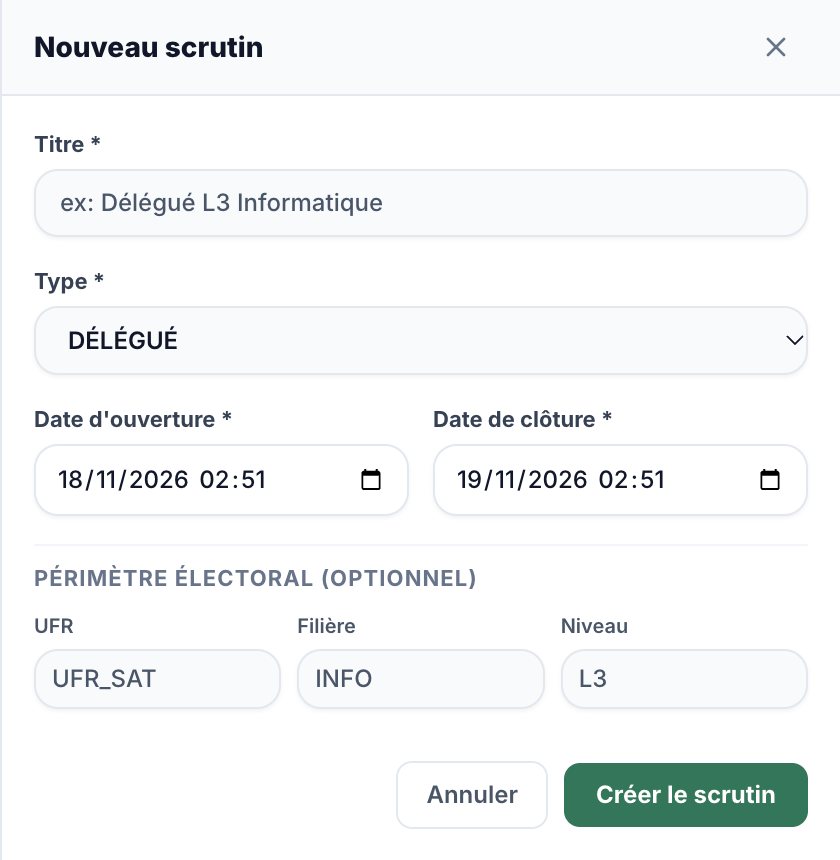
\includegraphics[width=\textwidth,height=0.38\textheight,keepaspectratio]{3-2-5-admin-nouveau-scrutin.png}
        \caption{Drawer de création d'un scrutin}
        \label{fig:admin-new}
    \end{minipage}
    \hfill
    \begin{minipage}{0.48\textwidth}
        \centering
        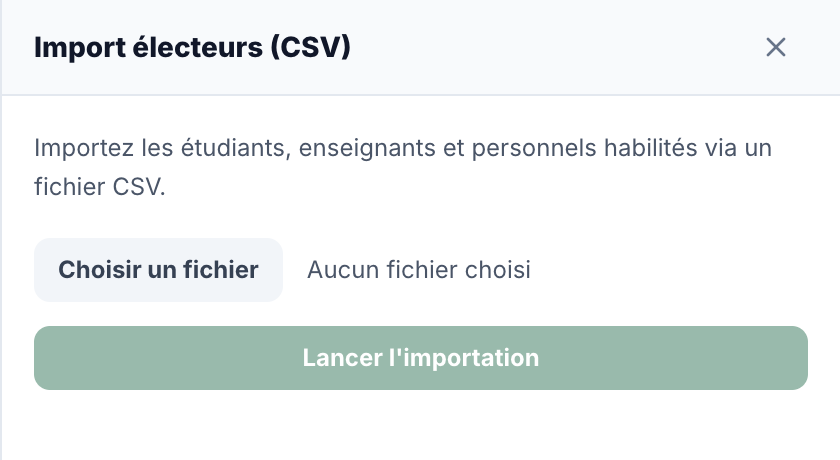
\includegraphics[width=\textwidth,height=0.38\textheight,keepaspectratio]{3-2-5-admin-import-csv.png}
        \caption{Import CSV des utilisateurs et résultat}
        \label{fig:admin-csv}
    \end{minipage}
\end{figure}

\begin{figure}[H]
    \centering
    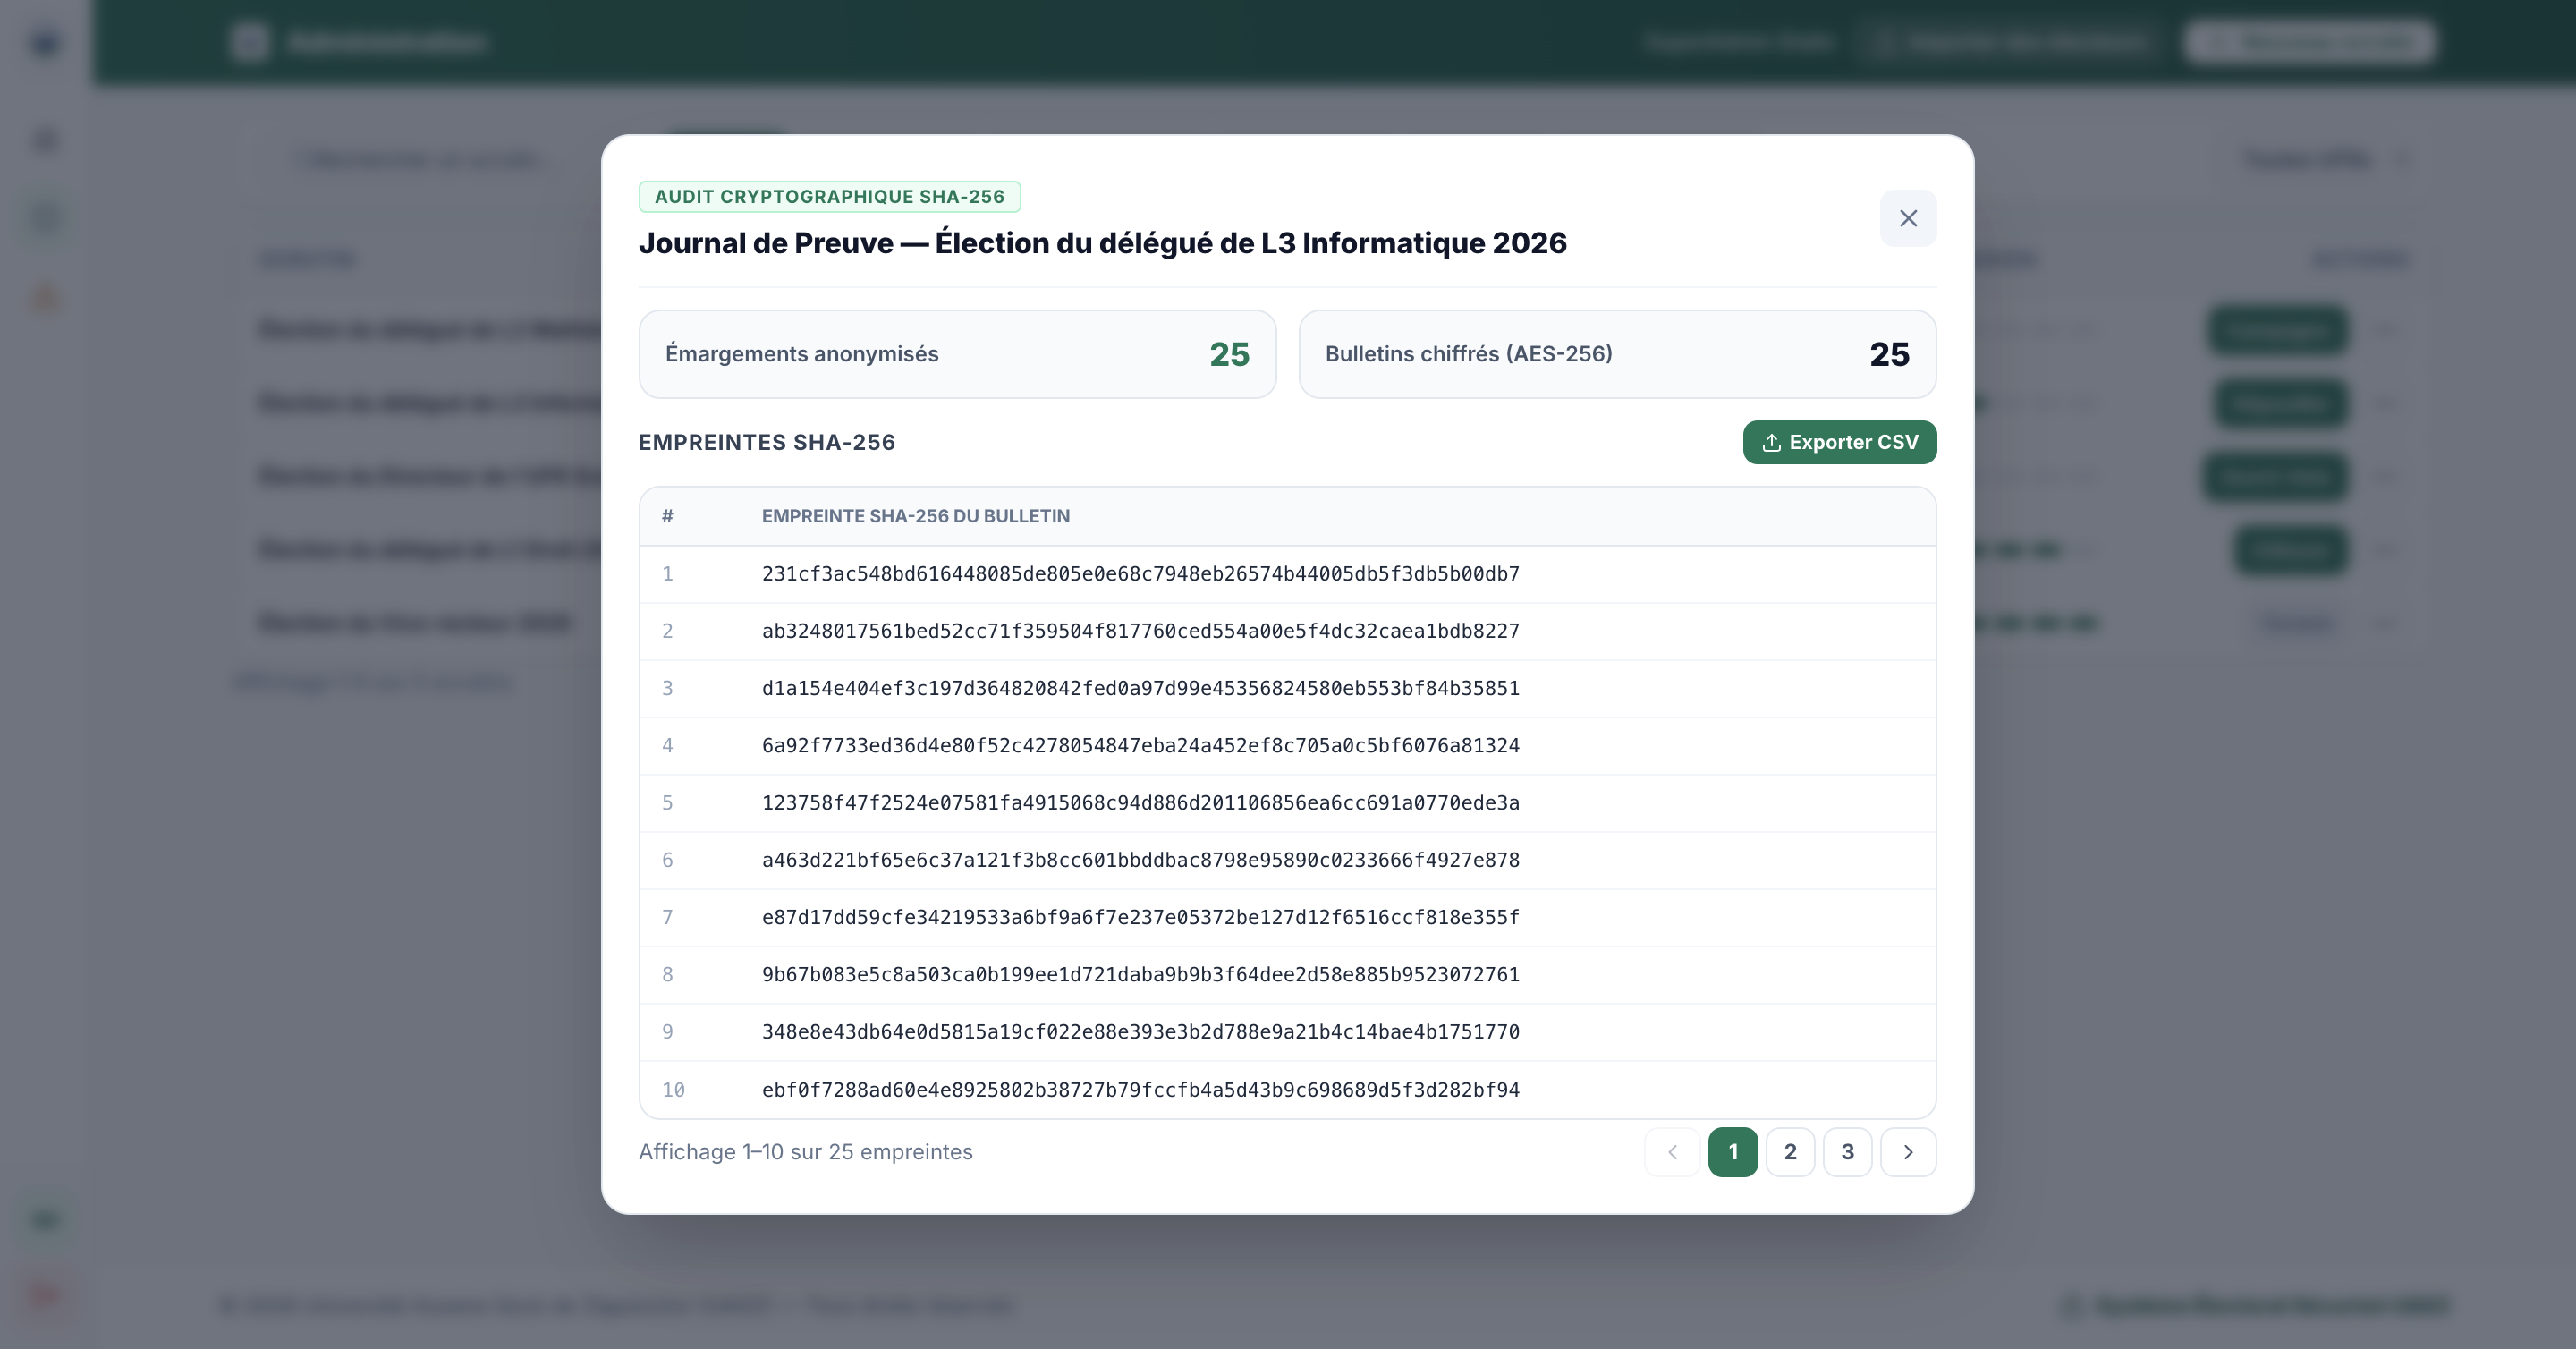
\includegraphics[width=0.92\textwidth,height=0.44\textheight,keepaspectratio]{3-2-5-admin-audit.png}
    \caption{Journal d'audit SHA-256 et export CSV (\texttt{/admin})}
    \label{fig:admin-audit}
\end{figure}

\begin{figure}[H]
    \centering
    \begin{minipage}{0.48\textwidth}
        \centering
        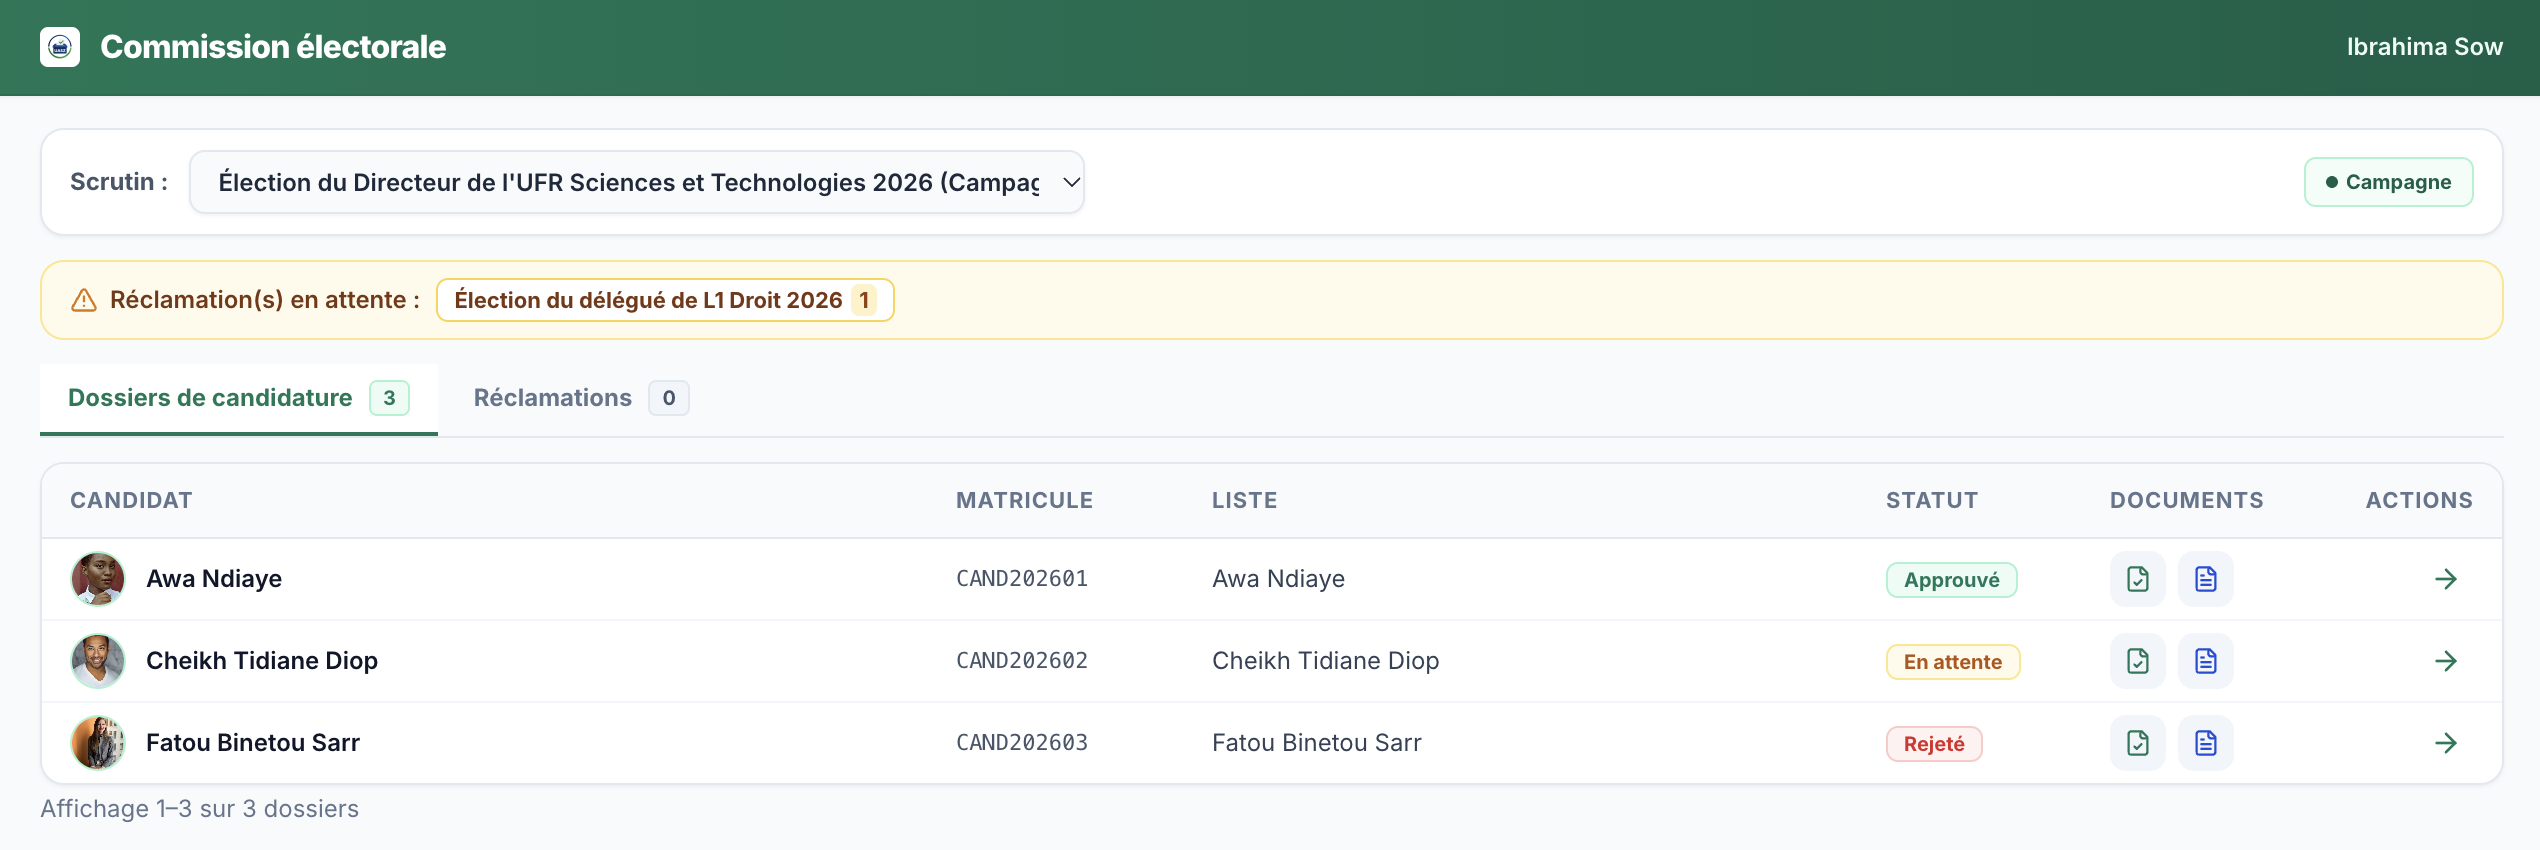
\includegraphics[width=\textwidth,height=0.38\textheight,keepaspectratio]{3-2-6-commission-dossiers.png}
        \caption{Commission : dossiers de candidatures}
        \label{fig:comm-dossiers}
    \end{minipage}
    \hfill
    \begin{minipage}{0.48\textwidth}
        \centering
        
\includegraphics[width=\textwidth,height=0.38\textheight,keepaspectratio]{3-2-6-commission-drawer.png}
        \caption{Drawer de validation / rejet motivé}
        \label{fig:comm-drawer}
    \end{minipage}
\end{figure}

\begin{figure}[H]
    \centering
    \begin{minipage}{0.48\textwidth}
        \centering
        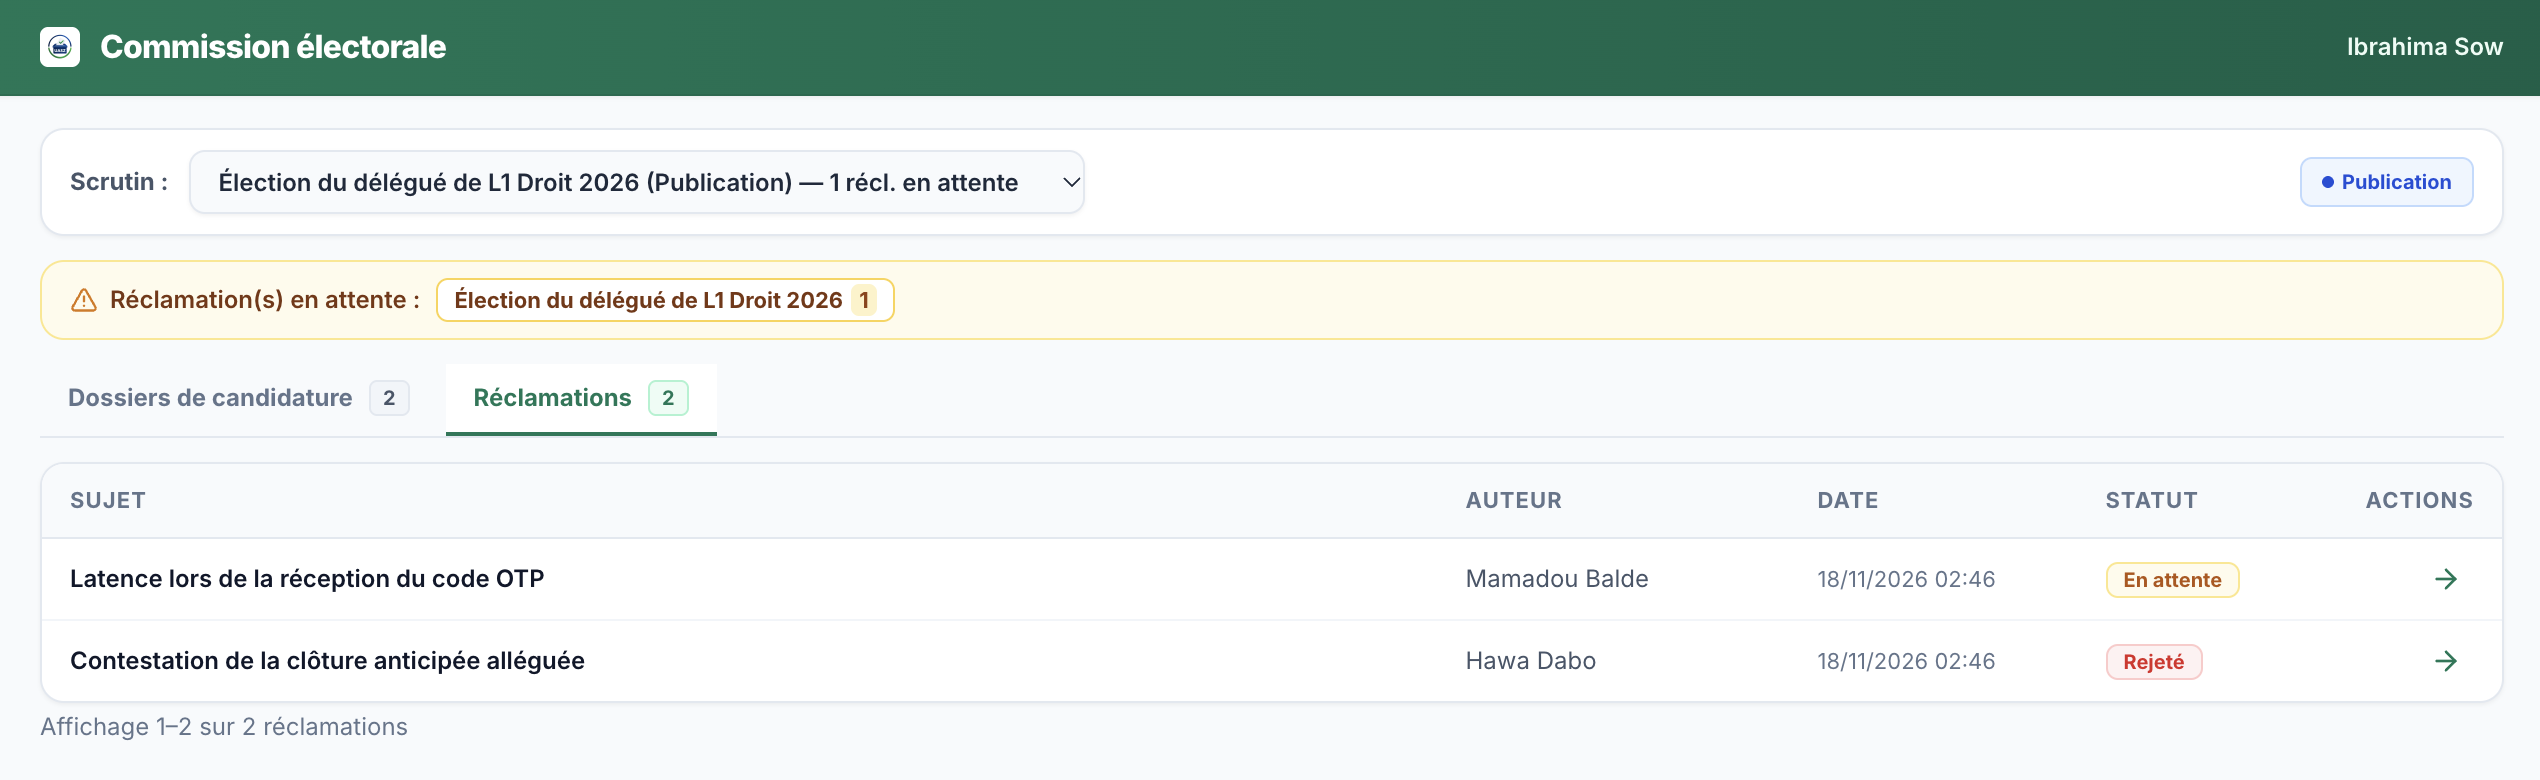
\includegraphics[width=\textwidth,height=0.38\textheight,keepaspectratio]{3-2-6-commission-reclamations.png}
        \caption{Traitement des réclamations (Commission)}
        \label{fig:comm-reclam}
    \end{minipage}
    \hfill
    \begin{minipage}{0.48\textwidth}
        \centering
        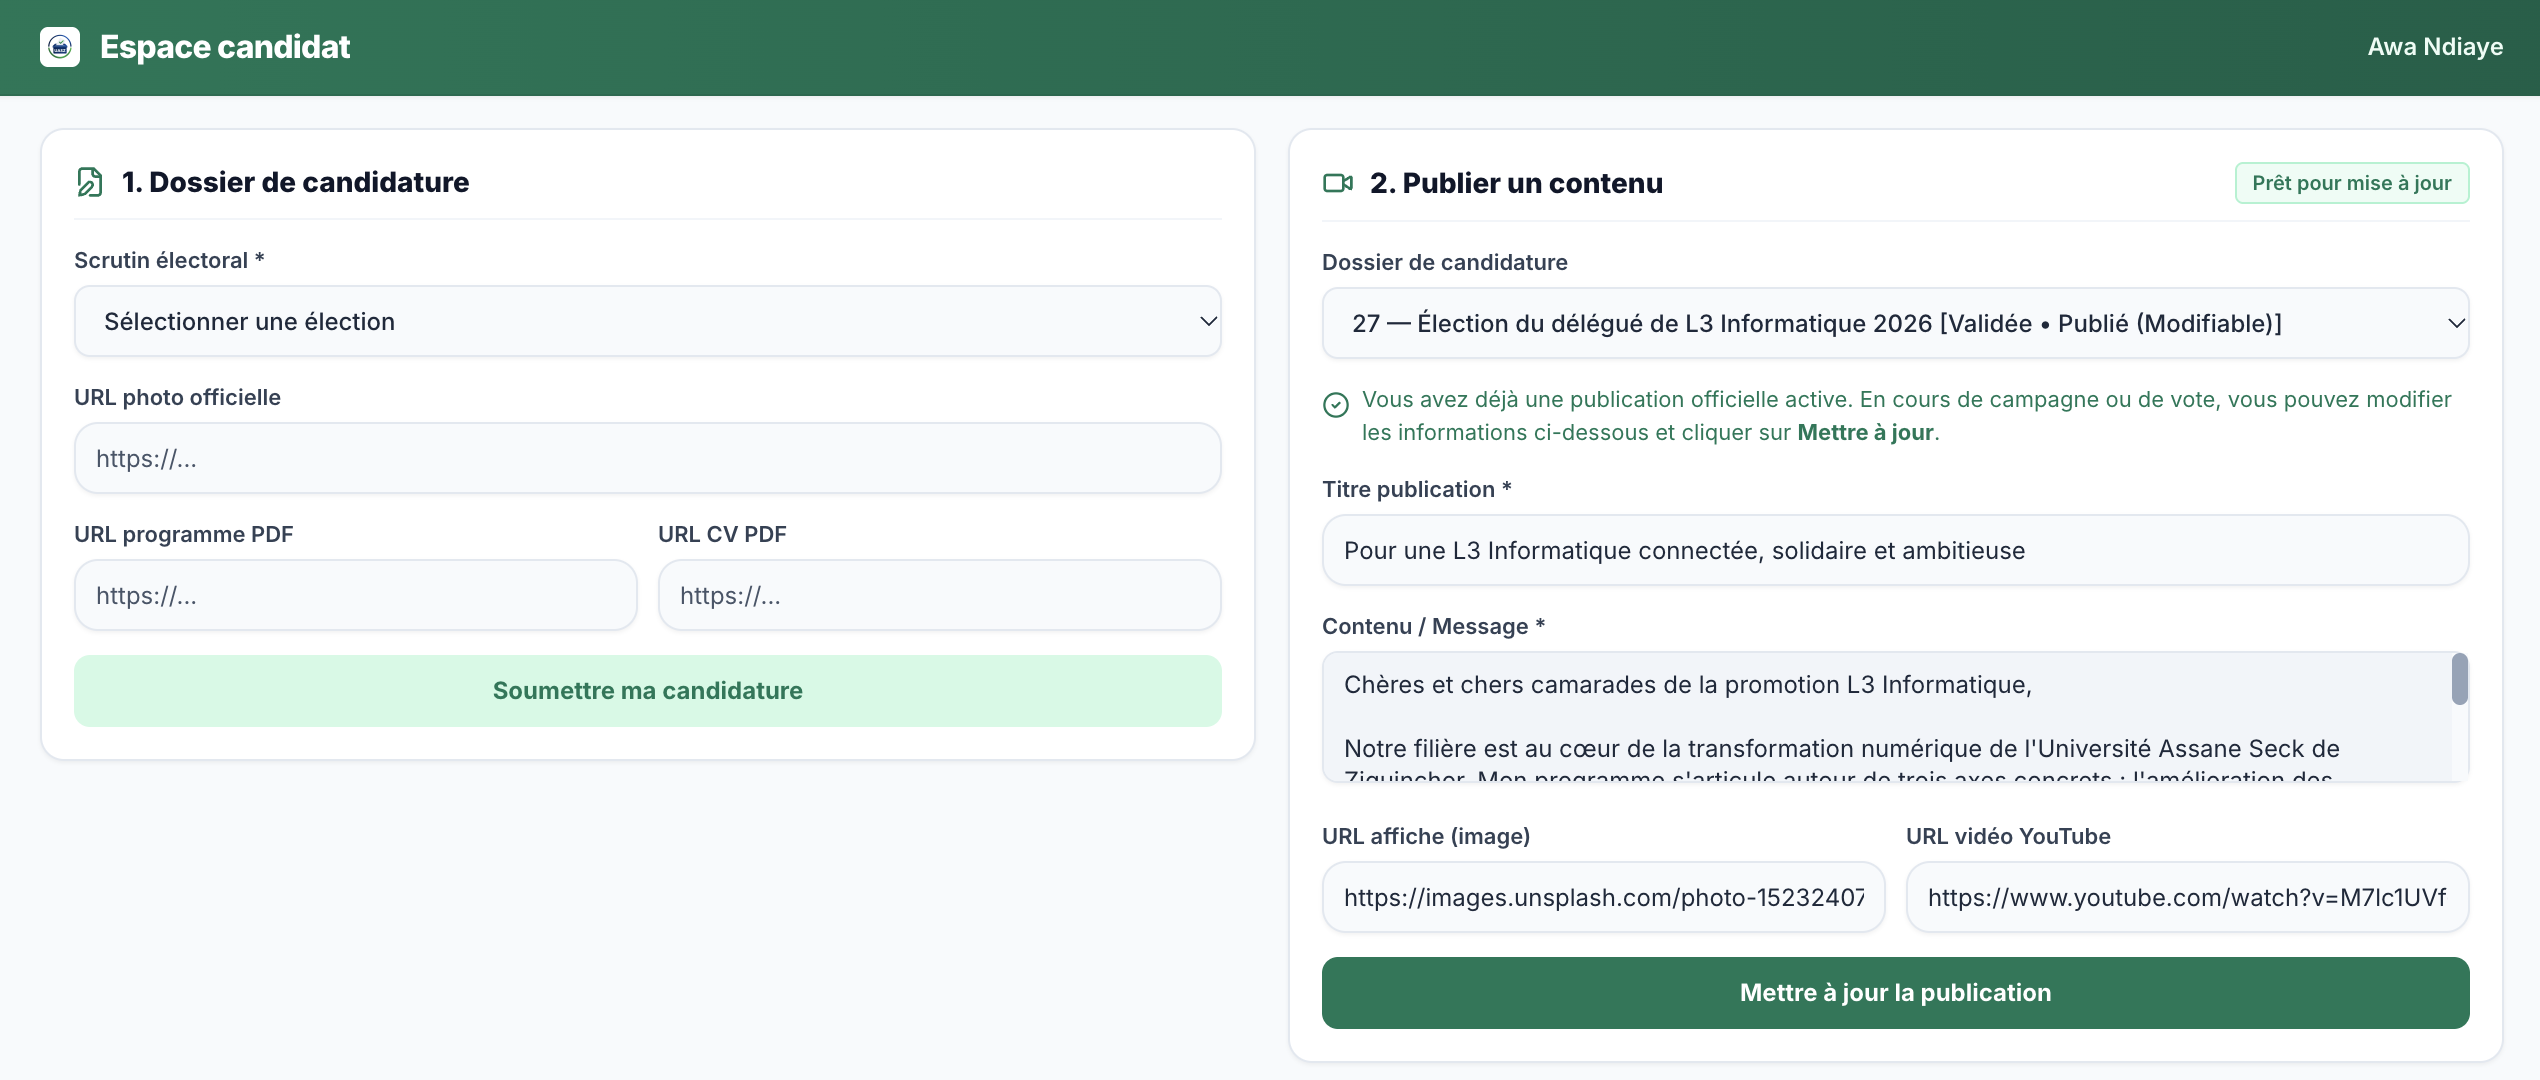
\includegraphics[width=\textwidth,height=0.38\textheight,keepaspectratio]{3-2-7-candidat-espace.png}
        \caption{Espace Candidat (\texttt{/candidat})}
        \label{fig:cand-espace}
    \end{minipage}
\end{figure}

\begin{figure}[H]
    \centering
    \begin{minipage}{0.62\textwidth}
        \centering
        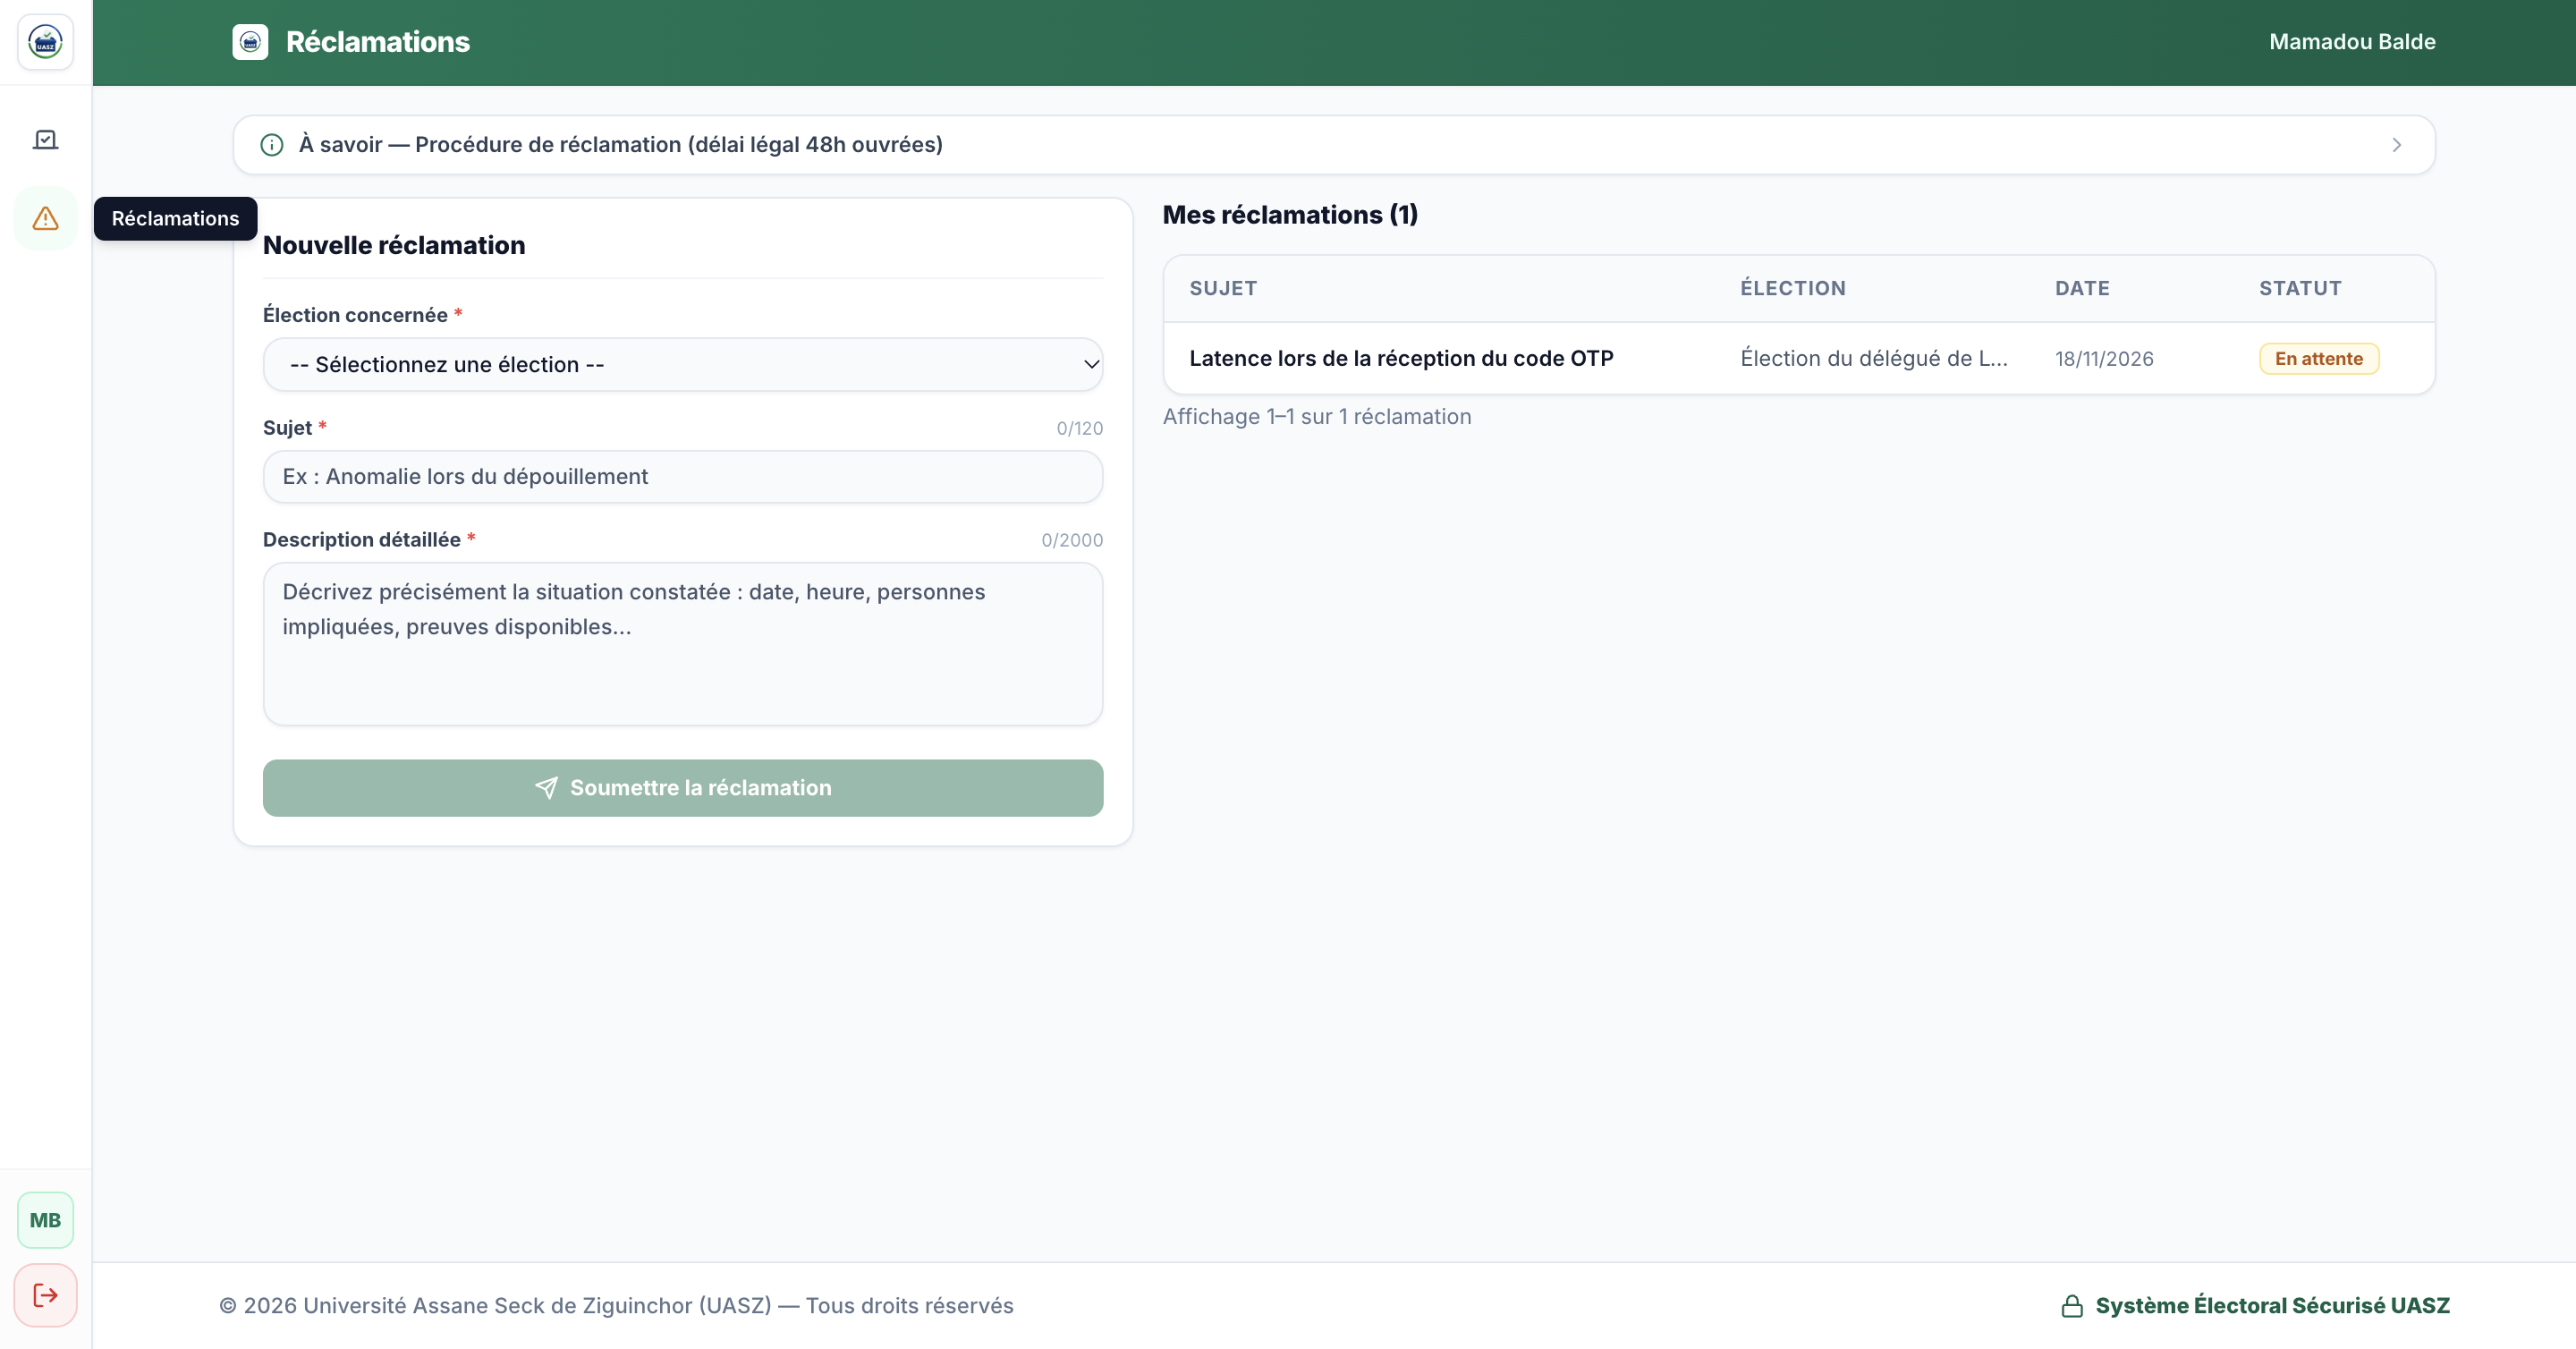
\includegraphics[width=\textwidth,height=0.40\textheight,keepaspectratio]{3-2-8-reclamations-electeur.png}
        \caption{Réclamations côté électeur (\texttt{/reclamations})}
        \label{fig:reclam-elec}
    \end{minipage}
    \hfill
    \begin{minipage}{0.34\textwidth}
        \centering
        
\includegraphics[width=\textwidth,height=0.40\textheight,keepaspectratio]{3-2-8-reclamations-mobile.png}
        \caption{Réclamations mobile (\texttt{390x844})}
        \label{fig:reclam-mob}
    \end{minipage}
\end{figure}

\begin{figure}[H]
    \centering
    \begin{minipage}{0.46\textwidth}
        \centering
        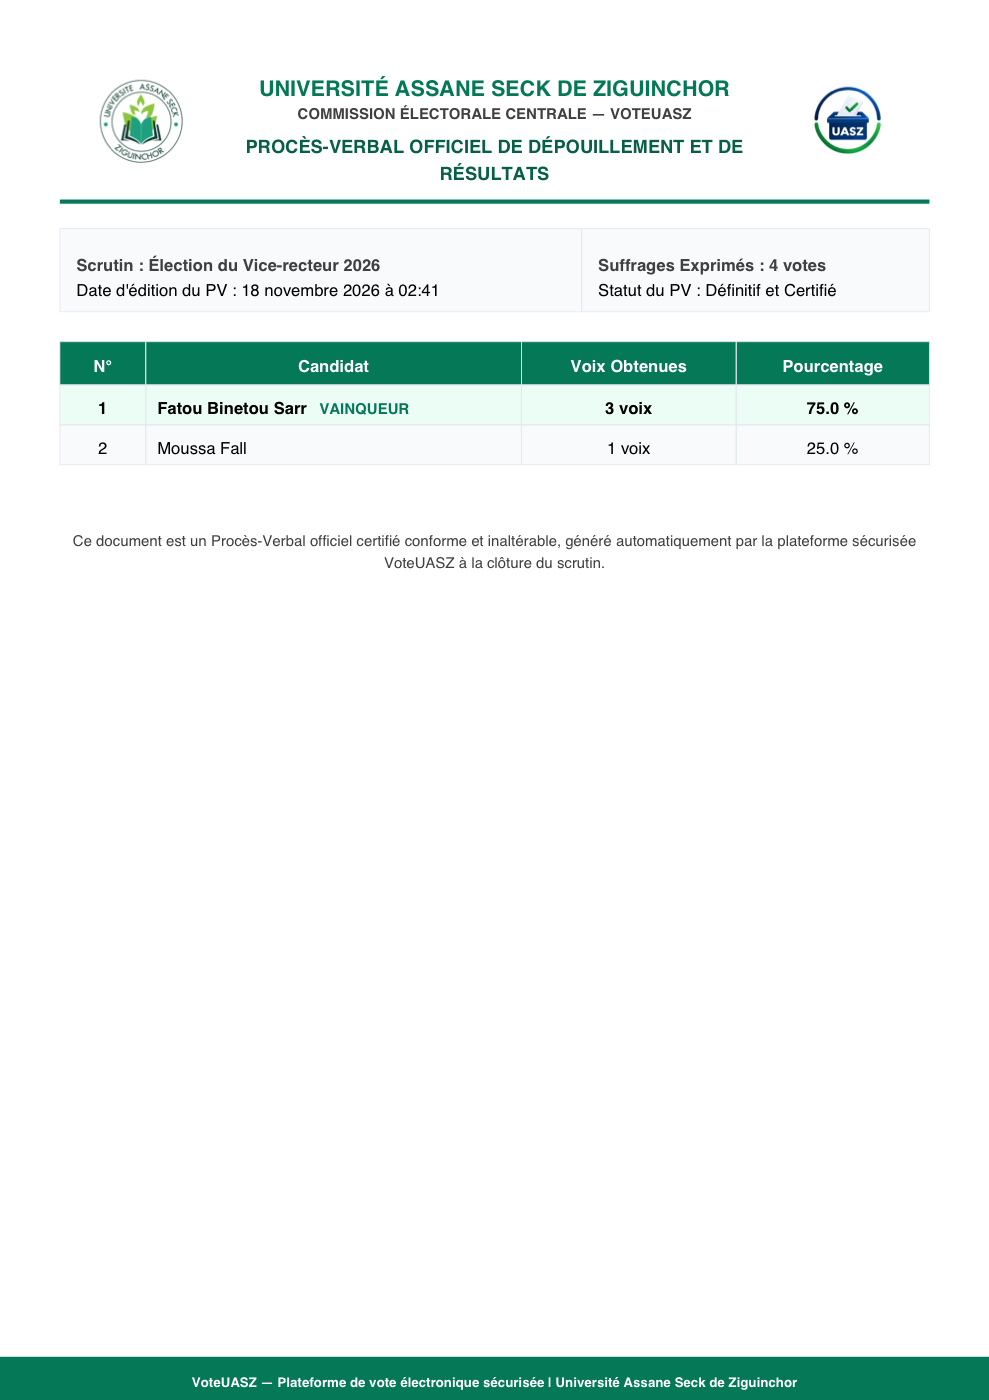
\includegraphics[width=\textwidth,height=0.44\textheight,keepaspectratio]{3-2-9-pv-pdf.png}
        \caption{Procès-Verbal PDF généré (\textit{Vice-recteur 2026})}
        \label{fig:pv-pdf}
    \end{minipage}
    \hfill
    \begin{minipage}{0.50\textwidth}
        \centering
        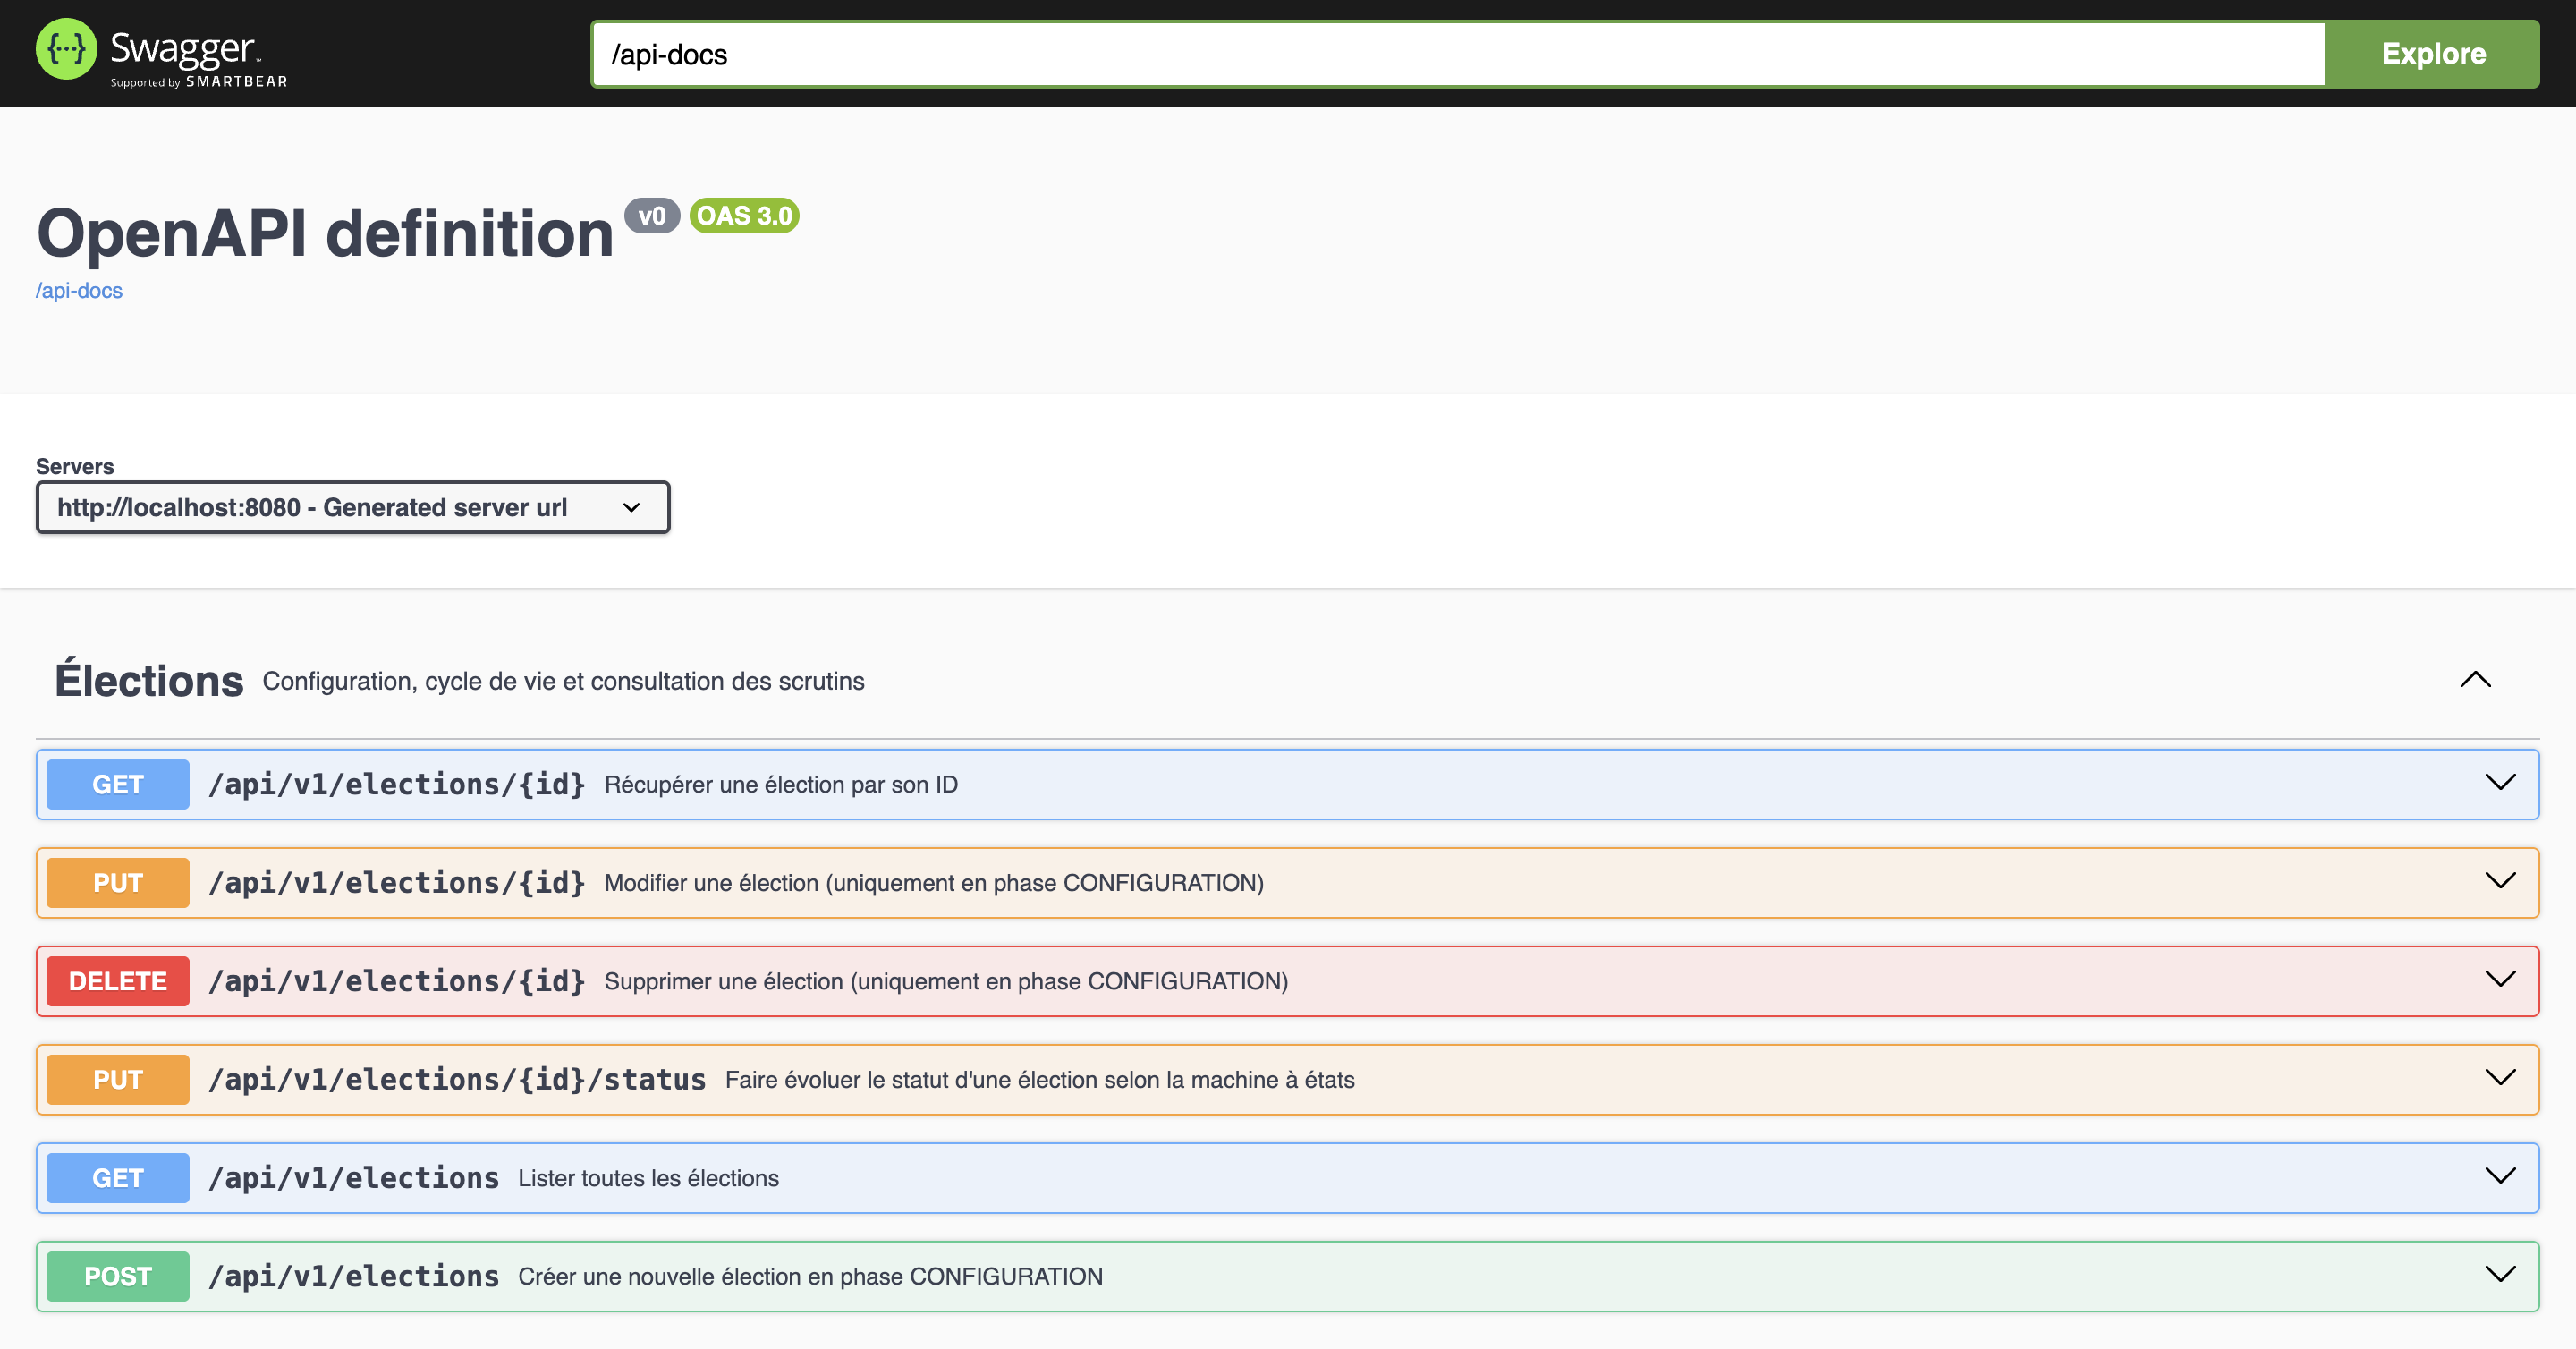
\includegraphics[width=\textwidth,height=0.44\textheight,keepaspectratio]{3-2-10-swagger-ui.png}
        \caption{Swagger UI (capture locale \texttt{localhost:8080})}
        \label{fig:swagger}
    \end{minipage}
\end{figure}

\section{Tests, qualité et critères de validation}

\subsection{Suite de tests Backend (\texttt{mvn -B verify})}
Exécutée sous Java 21, la commande \texttt{mvn -B verify} valide :
\begin{itemize}
    \item \textbf{Tests JUnit / Spring Boot} : \textbf{122 tests exécutés, 0 échec, 0 erreur, 0 ignoré} (\texttt{BUILD SUCCESS}).
    \item \textbf{Couverture JaCoCo 0.8.11 (50 classes)} : Instructions \textbf{74,30\,\%} (\texttt{5\,632/7\,580}), Branches \textbf{57,10\,\%} (\texttt{358/627}), Lignes \textbf{74,68\,\%} (\texttt{1\,233/1\,651}), Méthodes \textbf{70,39\,\%} (\texttt{164/233}), Classes \textbf{94,00\,\%} (\texttt{47/50}) (figure~\ref{fig:jacoco}).
    \item \textbf{Checkstyle 3.3.1} : \textbf{0 violation} (\texttt{backend/checkstyle.xml}).
\end{itemize}

\begin{figure}[H]
    \centering
    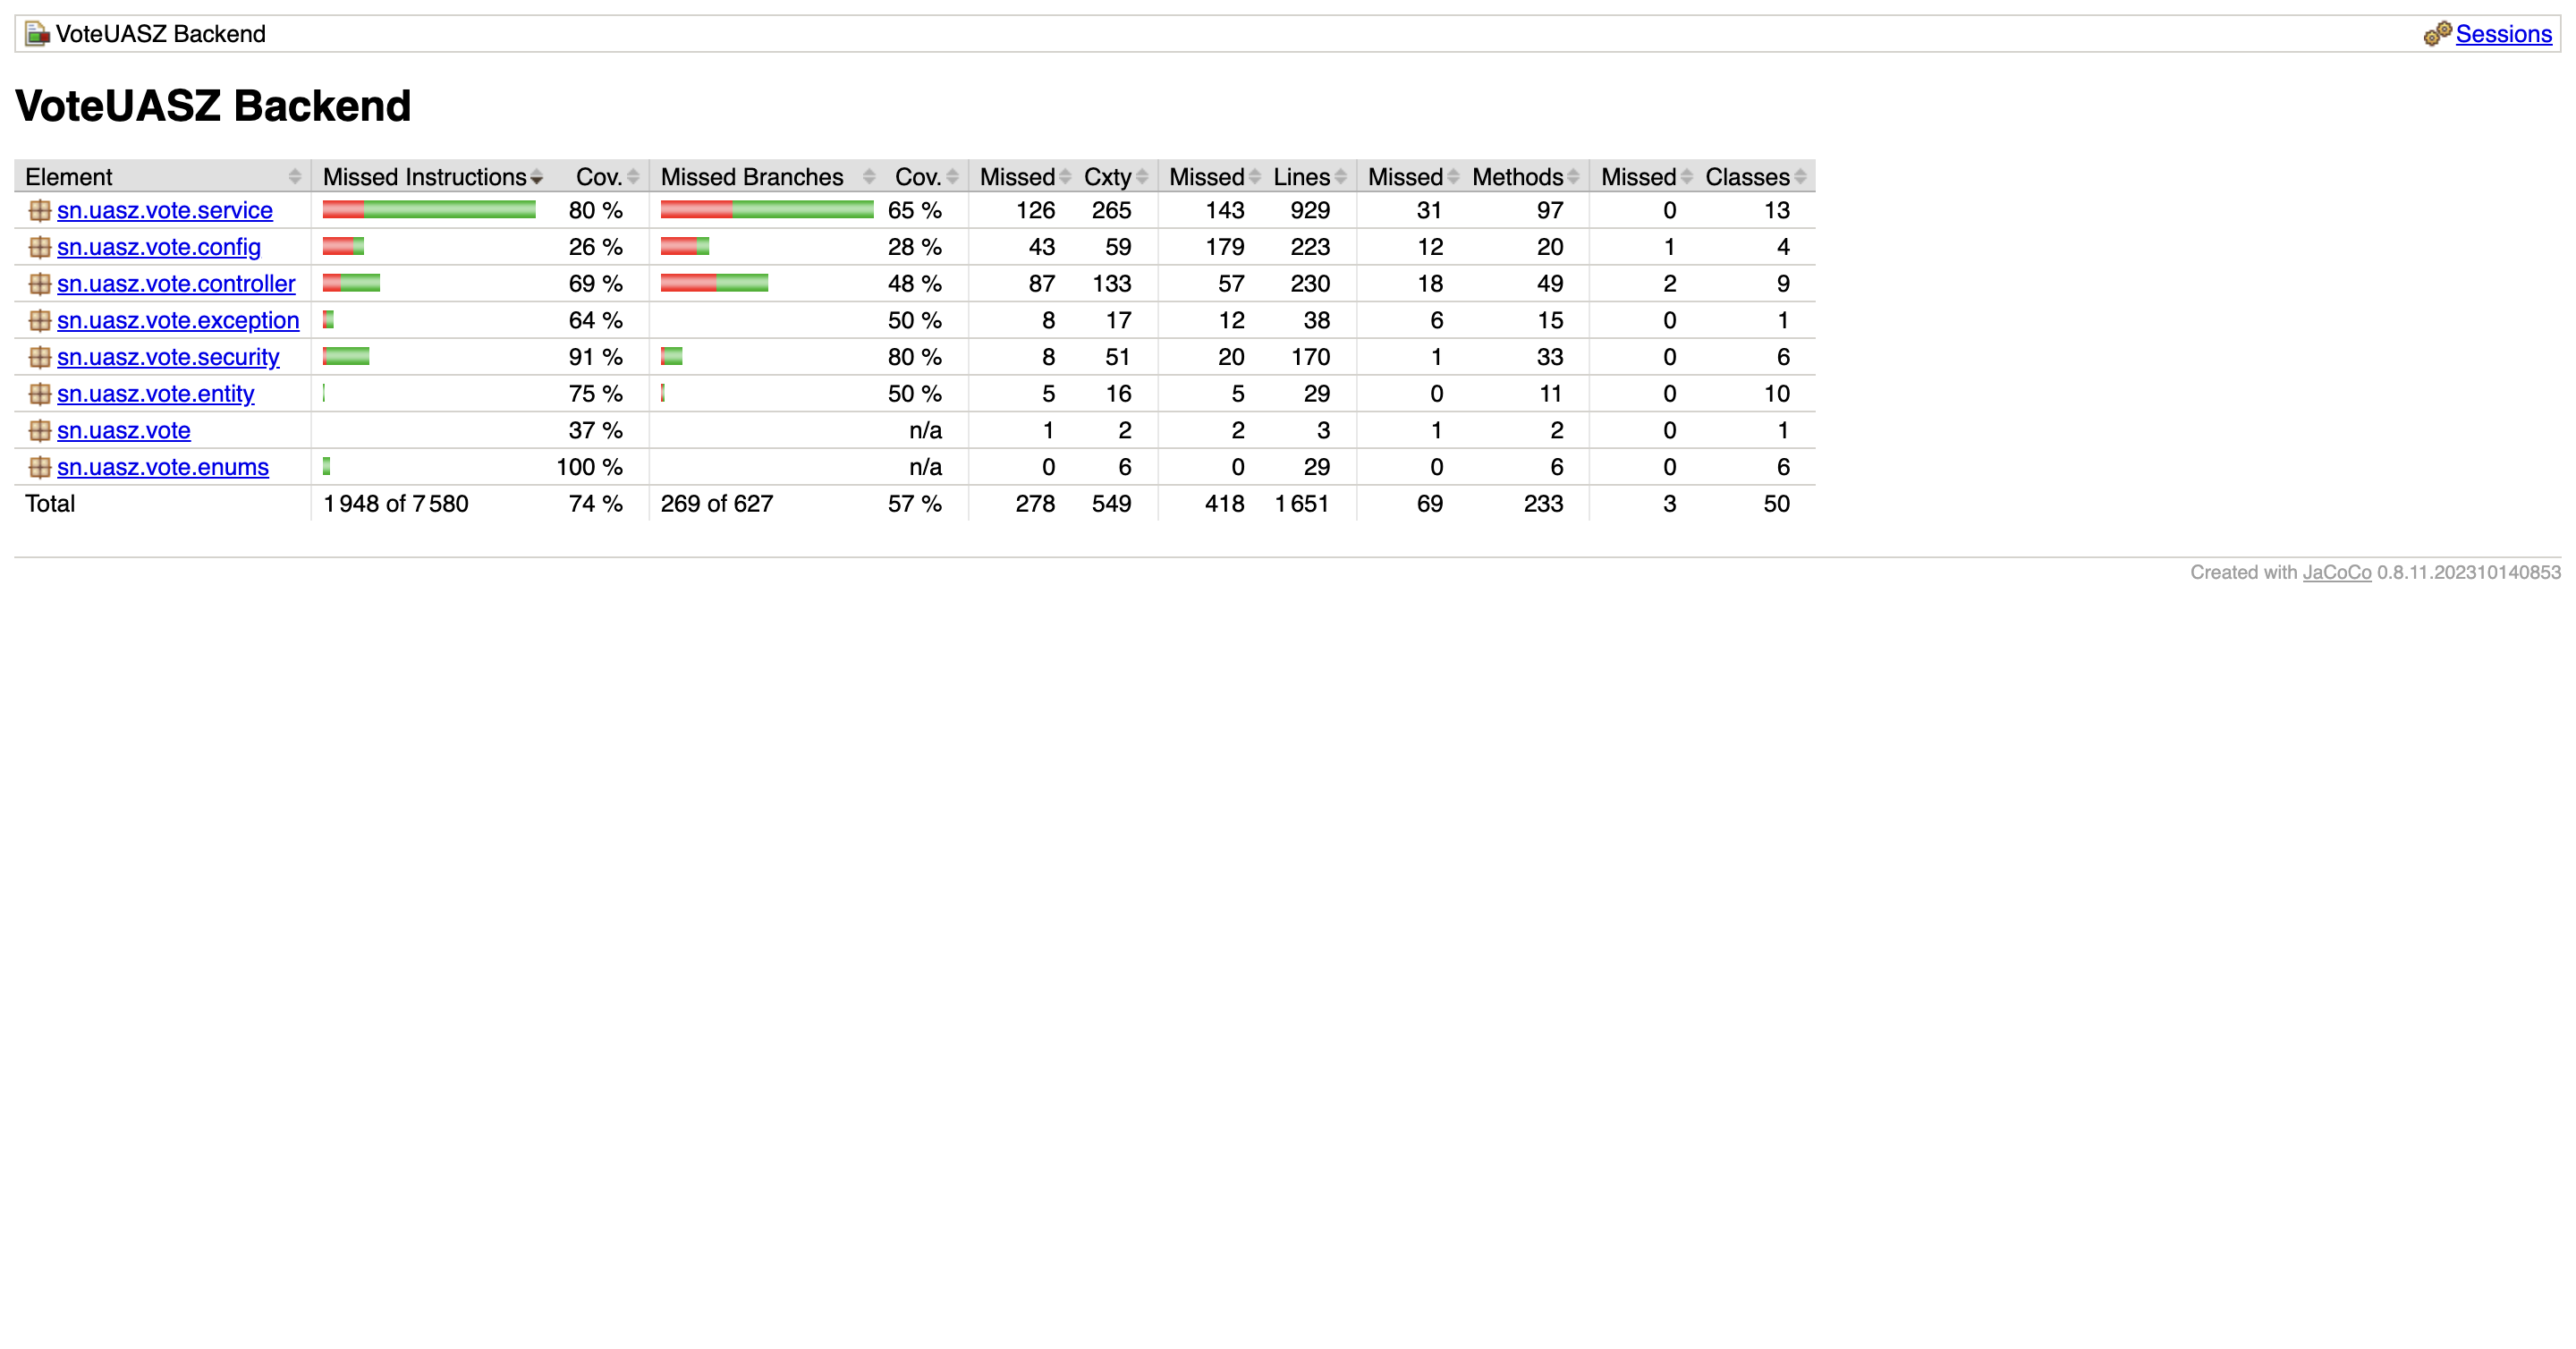
\includegraphics[width=0.92\textwidth,height=0.38\textheight,keepaspectratio]{4-1-jacoco.png}
    \caption{Rapport de couverture JaCoCo généré par \texttt{mvn -B verify}}
    \label{fig:jacoco}
\end{figure}

\subsection{Tests Frontend Angular et taille du bundle}
\begin{itemize}
    \item \textbf{Tests Karma/Jasmine (\texttt{ng test})} : \textbf{26 tests exécutés, 26 succès, 0 échec}.
    \item \textbf{Build de production (\texttt{ng build --configuration production})} : bundle initial total de \textbf{419,65\,kB} (\textbf{109,08\,kB} transférés) et \textbf{12 chunks} chargés à la demande.
\end{itemize}

\subsection{Synthèse des critères de validation}
\begin{table}[H]
\centering
\caption{Critères de validation : méthode et résultat réel mesuré}
\label{tab:criteres-validation}
\small
\begin{tabularx}{\textwidth}{@{}llX@{}}
\toprule
\rowcolor{uaszlight}
\textbf{Critère} & \textbf{Méthode} & \textbf{Résultat mesuré} \\
\midrule
Logique métier & \texttt{mvn -B verify} & \textbf{Réussi} : 122/122 tests, 74,30\,\% instructions, 0 violation Checkstyle. \\
Composants UI & \texttt{ng test} (ChromeHeadless) & \textbf{Réussi} : 26/26 tests passés. \\
Taille bundle & \texttt{ng build --configuration production} & \textbf{Réussi} : 419,65\,kB initial (109,08\,kB transférés). \\
Chaîne des bulletins & \texttt{AuditService.verifyBallotChain()} & \textbf{Réussi} : \texttt{chainValid=true} sur 25 + 3 + 4 bulletins réels. \\
Charge (\texttt{k6}) & Script \texttt{perf/load-test.js} & \textbf{Non testé} (\texttt{k6} non installé sur la machine locale). \\
Scan OWASP ZAP & \texttt{.github/workflows/zap-baseline.yml} & \textbf{Non testé} localement (workflow manuel GitHub Actions). \\
Performance 3G & Lighthouse avec throttling 3G & \textbf{Non testé} (à exécuter sur l'environnement de production). \\
\bottomrule
\end{tabularx}
\end{table}

\section{Déploiement Cloud}

Le déploiement continu s'appuie sur \texttt{render.yaml} (service Docker Java 21 + base PostgreSQL 16 \texttt{voteuasz-db} sur Render, avec variables \texttt{JWT\_SECRET}, \texttt{CRYPTO\_SECRET}, \texttt{AUDIT\_IP\_SALT} et \texttt{BREVO\_API\_KEY}) et \texttt{vercel.json} (build Angular 17 et réécriture \texttt{/api/(.*)} vers le backend Render). L'environnement local est orchestré via \texttt{docker-compose.yml} (PostgreSQL 16 sur port 5540 et MailHog sur ports 1025/8025).

\section{Synthèse vs cahier des charges, écarts justifiés et limites}

\begin{table}[H]
\centering
\caption{Écarts justifiés entre le cahier des charges initial et le code réel}
\label{tab:ecarts}
\small
\begin{tabularx}{\textwidth}{@{}lXX@{}}
\toprule
\rowcolor{uaszlight}
\textbf{Fonction prévue} & \textbf{Implémentation réelle} & \textbf{Justification} \\
\midrule
OTP par SMS & OTP par e-mail (Brevo HTTPS API / SMTP) & Absence de passerelle SMS payante ; l'e-mail institutionnel reste gratuit et traçable. \\
Export PV JasperReports & Génération programmatique via OpenPDF 1.3.30 & Poids réduit, aucune dépendance à un moteur \texttt{.jrxml} externe. \\
Upload binaire médias & URLs externes (\texttt{photoUrl}, \texttt{programmePdf}, \texttt{cvUrl}, \texttt{afficheUrl}) & Système de fichiers éphémère sur Render Free sans stockage objet S3/Cloudinary. \\
Tests CI Testcontainers & Base H2 en mémoire (\texttt{@Profile("test")}) & Exécution rapide sans démon Docker requis en CI. \\
Mode hors-ligne complet & PWA Angular (\texttt{ngsw-config.json}) pour les assets & Le dépôt de vote nécessite une validation OTP et transactionnelle en ligne. \\
\bottomrule
\end{tabularx}
\end{table}

\chapter*{Conclusion Générale}
\addcontentsline{toc}{chapter}{Conclusion Générale}

Le projet \textbf{VoteUASZ} répond au besoin de dématérialisation des scrutins de l'Université Assane Seck de Ziguinchor en proposant une application web complète, de l'import CSV des électeurs à la génération du procès-verbal PDF.

Sur le plan technique, l'architecture sépare l'émargement (\texttt{VoterAuditLog}) du bulletin (\texttt{Ballot} sans clé étrangère vers \texttt{User}), chiffre les bulletins en \textbf{AES-256-GCM} (PBKDF2), relie la chaîne des bulletins en \textbf{SHA-256}, sécurise l'accès par \textbf{JWT HS256} avec \textbf{Refresh Token} rotatif et OTP e-mail, et diffuse les résultats en temps réel via \textbf{STOMP} et \textbf{Chart.js}. La qualité est vérifiée par \textbf{122 tests backend} (couverture JaCoCo \textbf{74,30\,\%} en instructions, \textbf{0 violation Checkstyle}) et \textbf{26 tests frontend} (\textbf{0 échec}).

De manière lucide, certaines garanties restent perfectibles (clé AES portée par le serveur, corrélation d'ordre possible entre l'ID séquentiel d'émargement et \texttt{sequenceNumber}, absence de signature RSA/X.509 du PV PDF), ouvrant la voie à des perspectives claires pour une version ultérieure.

% ============================================================================
% BIBLIOGRAPHIE
% ============================================================================
\begin{thebibliography}{9}
\addcontentsline{toc}{chapter}{Bibliographie}

\bibitem{spring-boot}
VMware Tanzu, \textit{Spring Boot 3.2.3 Reference Documentation}, 2024. \url{https://docs.spring.io/spring-boot/docs/3.2.3/reference/html/}

\bibitem{spring-security}
VMware Tanzu, \textit{Spring Security Reference}, 2024. \url{https://docs.spring.io/spring-security/reference/}

\bibitem{angular}
Google, \textit{Angular 17 Documentation}, 2024. \url{https://angular.io/docs}

\bibitem{postgresql}
PostgreSQL Global Development Group, \textit{PostgreSQL 16 Documentation}, 2024. \url{https://www.postgresql.org/docs/16/}

\bibitem{nist-gcm}
NIST, \textit{Recommendation for Block Cipher Modes of Operation: Galois/Counter Mode (GCM) -- SP 800-38D}, 2007.

\bibitem{rfc7519}
M. Jones, J. Bradley, N. Sakimura, \textit{JSON Web Token (JWT) -- RFC 7519}, IETF, 2015.

\bibitem{openpdf}
LibrePDF, \textit{OpenPDF 1.3.30 Documentation}, GitHub. \url{https://github.com/LibrePDF/OpenPDF}

\bibitem{owasp}
OWASP Foundation, \textit{OWASP Top 10 Web Application Security Risks}, 2021. \url{https://owasp.org/www-project-top-ten/}

\end{thebibliography}

% ============================================================================
% ANNEXES
% ============================================================================
\appendix

\chapter{Localisation des algorithmes et contrat OpenAPI}

\begin{table}[H]
\centering
\caption{Localisation des algorithmes clés dans le backend}
\small
\begin{tabularx}{\textwidth}{@{}lXl@{}}
\toprule
\rowcolor{uaszlight}
\textbf{Mécanisme} & \textbf{Fichier} & \textbf{Lignes} \\
\midrule
Vérification OTP \& \texttt{VoteToken} & \texttt{service/VotingService.java} & \texttt{L94--L142} \\
Transaction de vote \& chaînage SHA-256 & \texttt{service/VotingService.java} & \texttt{L150--L228} \\
Chiffrement AES-256-GCM \& PBKDF2 & \texttt{service/CryptoService.java} & \texttt{L62--L82, L130--L139} \\
Vérification chaîne de hash & \texttt{service/AuditService.java} & \texttt{L52--L77} \\
Refresh token \& mot de passe & \texttt{controller/AuthController.java} & \texttt{L107--L240} \\
Machine à états (6 états) & \texttt{service/ElectionStateMachine.java} & \texttt{L10--L35} \\
\bottomrule
\end{tabularx}
\end{table}

\begin{table}[H]
\centering
\caption{Principaux endpoints REST (\texttt{docs/openapi.yaml}, préfixe \texttt{/api/v1})}
\small
\begin{tabularx}{\textwidth}{@{}llX@{}}
\toprule
\rowcolor{uaszlight}
\textbf{Module} & \textbf{Endpoints} & \textbf{Accès} \\
\midrule
Authentification & \texttt{POST /auth/login}, \texttt{/refresh}, \texttt{/logout}, \texttt{/forgot-password}, \texttt{/reset-password} & Public (sauf \texttt{change-password}) \\
Scrutins & \texttt{GET /elections}, \texttt{POST/PUT/DELETE /elections}, \texttt{PUT /elections/\{id\}/status} & Public en lecture ; \texttt{SUPER\_ADMIN} en écriture \\
Candidatures & \texttt{POST /candidacies}, \texttt{GET /candidacies/election/\{id\}}, \texttt{PUT /.../validate} & \texttt{CANDIDAT} ; \texttt{COMMISSION} / \texttt{ADMIN} \\
Campagnes & \texttt{POST /campaigns}, \texttt{GET /campaigns/election/\{id\}} & \texttt{CANDIDAT} approuvé ; authentifié \\
Vote OTP & \texttt{POST /vote/request-otp}, \texttt{/verify-otp}, \texttt{/submit}, \texttt{GET /vote/status/\{id\}} & Électeur éligible authentifié \\
Résultats \& PV & \texttt{GET /results/\{id\}}, \texttt{GET /results/\{id\}/export-pdf} & Selon statut ; \texttt{ADMIN} / \texttt{COMMISSION} \\
Réclamations & \texttt{POST /complaints}, \texttt{GET /complaints/*}, \texttt{PUT /complaints/\{id\}/resolve} & Authentifié ; \texttt{COMMISSION} / \texttt{ADMIN} \\
Audit \& Import & \texttt{GET /audit/\{id\}}, \texttt{/export-csv}, \texttt{POST /admin/users/import-csv} & \texttt{SUPER\_ADMIN} / \texttt{COMMISSION} \\
\bottomrule
\end{tabularx}
\end{table}

\chapter{Guide d'installation locale et exemple d'audit / PV}

\section{Démarrage en local (Docker Compose + Angular)}
\begin{enumerate}
    \item Copier \texttt{.env.example} vers \texttt{.env} et renseigner \texttt{POSTGRES\_PASSWORD}, \texttt{JWT\_SECRET} (32+ car.), \texttt{CRYPTO\_SECRET} (32+ car.), \texttt{DEFAULT\_ELECTEUR\_PASSWORD} et \texttt{DEFAULT\_CANDIDAT\_PASSWORD}.
    \item Démarrer PostgreSQL 16 (port 5540) et MailHog (SMTP 1025, UI 8025) : \texttt{docker compose up -d postgres mailhog}.
    \item Lancer le backend Java 21 : \texttt{mvn spring-boot:run} (ou \texttt{java -jar vote-uasz-backend-1.0.0.jar}) dans \texttt{backend/}.
    \item Lancer le frontend Angular 17 : \texttt{cd frontend \&\& npm ci \&\& npx ng serve --port 4200}.
\end{enumerate}

\section{Exemple d'export CSV d'audit et de PV PDF}
Lors du jeu de données local de démonstration (scrutin \textit{Élection du délégué de L3 Informatique 2026}, 25 votes enregistrés), l'appel à \texttt{AuditService.verifyBallotChain()} retourne \texttt{chainValid = true} avec 25 bulletins chaînés depuis \texttt{"GENESIS"} et 25 émargements anonymisés. Le procès-verbal généré pour \textit{Élection du Vice-recteur 2026} (\texttt{CLOTURE}) est présenté en figure~\ref{fig:pv-pdf} (chapitre 3).


\end{document}
